% Формат А4, 14pt (ГОСТ Р 7.0.11-2011, 5.3.6)
\documentclass[a4paper,14pt]{extreport}

%%%%%%%%%%%%%%%%%%%%%%%%%%%%%%%%%%%%%%%%%%%%%%%%%%%%%%
%%%% Файл упрощённых настроек шаблона диссертации %%%%
%%%%%%%%%%%%%%%%%%%%%%%%%%%%%%%%%%%%%%%%%%%%%%%%%%%%%%

%%%        Подключение пакетов                 %%%
\usepackage{ifthen}                 % добавляет ifthenelse
%%% Инициализирование переменных, не трогать!  %%%
\newcounter{intvl}
\newcounter{otstup}
\newcounter{contnum}
\newcounter{pgnum}
\newcounter{bibliosel}
\newcounter{chapstyle}
\newcounter{headingdelim}
\newcounter{headingalign}
\newcounter{headingsize}
%%%%%%%%%%%%%%%%%%%%%%%%%%%%%%%%%%%%%%%%%%%%%%%%%%

%%% Область упрощённого управления оформлением %%%

%% Интервал между заголовками и между заголовком и текстом
% Заголовки отделяют от текста сверху и снизу тремя интервалами (ГОСТ Р 7.0.11-2011, 5.3.5)
\setcounter{intvl}{3}               % Коэффициент кратности к размеру шрифта

%% Отступы у заголовков в тексте
\setcounter{otstup}{0}              % 0 --- без отступа; 1 --- абзацный отступ

%% Нумерация формул, таблиц и рисунков
\setcounter{contnum}{0}             % 0 --- пораздельно (во введении подряд, без номера раздела); 1 --- сквозная нумерация по всей диссертации

%% Оглавление
\setcounter{pgnum}{1}               % 0 --- номера страниц никак не обозначены; 1 --- Стр. над номерами страниц (дважды компилировать после изменения)

%% Библиография
\setcounter{bibliosel}{0}           % 0 --- встроенная реализация с загрузкой файла через движок bibtex8; 1 --- реализация пакетом biblatex через движок biber

%% Текст и форматирование заголовков
\setcounter{chapstyle}{1}           % 0 --- разделы только под номером; 1 --- разделы с названием "Глава" перед номером
\setcounter{headingdelim}{1}        % 0 --- номер отделен пропуском в 1em или \quad; 1 --- номера разделов и приложений отделены точкой с пробелом, подразделы пропуском без точки; 2 --- номера разделов, подразделов и приложений отделены точкой с пробелом.

%% Выравнивание заголовков в тексте
\setcounter{headingalign}{0}        % 0 --- по центру; 1 --- по левому краю

%% Размеры заголовков в тексте
\setcounter{headingsize}{0}         % 0 --- по ГОСТ, все всегда 14 пт; 1 --- пропорционально изменяющийся размер в зависимости от базового шрифта
               % Упрощённые настройки шаблона 

%%% Проверка используемого TeX-движка %%%
\usepackage{iftex}
\newif\ifxetexorluatex   % определяем новый условный оператор (http://tex.stackexchange.com/a/47579/79756)
\ifXeTeX
    \xetexorluatextrue
\else
    \ifLuaTeX
        \xetexorluatextrue
    \else
        \xetexorluatexfalse
    \fi
\fi

%%% Поля и разметка страницы %%%
\usepackage{pdflscape}                              % Для включения альбомных страниц
\usepackage{geometry}                               % Для последующего задания полей

%%% Математические пакеты %%%
\usepackage{amsthm,amsfonts,amsmath,amssymb,amscd}  % Математические дополнения от AMS
\usepackage{mathtools}                              % Добавляет окружение multlined

%%%% Установки для размера шрифта 14 pt %%%%
%% Формирование переменных и констант для сравнения (один раз для всех подключаемых файлов)%%
%% должно располагаться до вызова пакета fontspec или polyglossia, потому что они сбивают его работу
\newlength{\curtextsize}
\newlength{\bigtextsize}
\setlength{\bigtextsize}{13.9pt}

\makeatletter
%\show\f@size                                       % неплохо для отслеживания, но вызывает стопорение процесса, если документ компилируется без команды  -interaction=nonstopmode 
\setlength{\curtextsize}{\f@size pt}
\makeatother

%%% Кодировки и шрифты %%%
\ifxetexorluatex
    \usepackage{polyglossia}                        % Поддержка многоязычности (fontspec подгружается автоматически)
\else
    \RequirePDFTeX                                  % tests for PDFTEX use and throws an error if a different engine is being used
    \usepackage{cmap}                               % Улучшенный поиск русских слов в полученном pdf-файле
    \usepackage[T2A]{fontenc}                       % Поддержка русских букв
    \usepackage[utf8]{inputenc}                     % Кодировка utf8
    \usepackage[english, russian]{babel}            % Языки: русский, английский
    \IfFileExists{pscyr.sty}{\usepackage{pscyr}}{}  % Красивые русские шрифты
\fi

%%% Оформление абзацев %%%
\usepackage{indentfirst}                            % Красная строка

%%% Цвета %%%
\usepackage[dvipsnames,usenames]{color}
\usepackage{colortbl}

%%% Таблицы %%%
\usepackage{longtable}                              % Длинные таблицы
\usepackage{multirow,makecell,array}                % Улучшенное форматирование таблиц
\usepackage{booktabs}                               % Возможность оформления таблиц в классическом книжном стиле (при правильном использовании не противоречит ГОСТ)
\usepackage[
singlelinecheck=false % <-- important
]{caption}

%%% Общее форматирование
\usepackage{soulutf8}                               % Поддержка переносоустойчивых подчёркиваний и зачёркиваний
\usepackage{icomma}                                 % Запятая в десятичных дробях


%%% Гиперссылки %%%
\usepackage{hyperref}

%%% Изображения %%%
\usepackage{graphicx}                               % Подключаем пакет работы с графикой

%%% Списки %%%
\usepackage{enumitem}

%%% Подписи %%%
\usepackage{caption}                                % Для управления подписями (рисунков и таблиц) % Может управлять номерами рисунков и таблиц с caption %Иногда может управлять заголовками в списках рисунков и таблиц
\usepackage{subcaption}                             % Работа с подрисунками и подобным

%%% Интервалы %%%
\usepackage[onehalfspacing]{setspace}               % Опция запуска пакета правит не только интервалы в обычном тексте, но и формульные

%%% Счётчики %%%
\usepackage[figure,table]{totalcount}               % Счётчик рисунков и таблиц
\usepackage{totcount}                               % Пакет создания счётчиков на основе последнего номера подсчитываемого элемента (может требовать дважды компилировать документ)
\usepackage{totpages}                               % Счётчик страниц, совместимый с hyperref (ссылается на номер последней страницы). Желательно ставить последним пакетом в преамбуле

  % Пакеты общие для диссертации и автореферата
%%% Колонтитулы %%%
\usepackage{fancyhdr}

%%% Прикладные пакеты %%% 
\usepackage{calc}               % Пакет для расчётов параметров, например длины
%\usepackage{etoolbox}          % ради функции patchcmd для управления списком литературы

\usepackage {interfaces-base}   % Набор базовых интерфейсов к некоторым пакетам, конкретные реализации загружаются в стиле

%%% Заголовки %%%
\usepackage{titlesec}           % Пакет настройки шрифтов заголовков в тексте

%%% Оглавление %%%
\usepackage{tocloft}

%%% Счётчики %%%
\usepackage{chngcntr}           % оперативная перенастройка счётчиков         % Пакеты для диссертации
\usepackage{tabularx,tabulary}  %таблицы с автоматически подбирающейся шириной столбцов


\usepackage{url}
\usepackage{hyperref}
\hypersetup{%
	colorlinks=true, 
	breaklinks=true, 
	urlcolor=blue, 
	linkcolor=blue, 
	citecolor=blue, 
} %%%

\usepackage{graphicx}
\usepackage{wrapfig}
\usepackage{lipsum}  % generates filler text

% Листинги с исходным кодом программ
\usepackage{fancyvrb}
\usepackage{listings}

% Плавающие окружения. во многом лучше пакета float
\usepackage{floatrow}
%Диаграммы Фейнмана
\usepackage{tikz}
\usetikzlibrary{trees}
\usetikzlibrary{decorations.pathmorphing}
\usetikzlibrary{decorations.markings}
\usetikzlibrary{positioning, automata, arrows, arrows.meta}

\usepackage{longtable} %Длинные таблицы
\usepackage{pdfpages}   %Вставлять пдф
\usepackage{afterpage} %Пустая страница
\usepackage{anyfontsize}

\usepackage{titlesec}
\usepackage{physics}
\DeclareMathOperator{\sinc}{sinc}

\pagestyle{fancy}
\fancyhf{}
%\fancyhead[LE,RO]{Share\LaTeX}
%\fancyhead[RE,LO]{Guides and tutorials}
%\fancyfoot[CE,CO]{\leftmark}
\fancyfoot[LE,RO]{\thepage}
\renewcommand{\headrulewidth}{0pt}

\usepackage{datatool}
%\usepackage{siunitx}
\usepackage{booktabs} % for nicer tables
%\usepackage{caption} % improve caption spacing (among other things)
\usepackage{bm}
\renewcommand*\dtldisplaystarttab{\toprule}
\renewcommand*\dtldisplayendtab{\tabularnewline\bottomrule}
\renewcommand*\dtldisplayafterhead{\midrule}

\usepackage{pgfplotstable}
\usepackage{siunitx}
\usepackage{booktabs}

\usepackage{hyperref}

\usepackage{fancyhdr}

        % Пакеты для специфических пользовательских задач
%%% Переопределение именований, чтобы можно было и в преамбуле использовать %%%
\renewcommand{\chaptername}{Глава}
\renewcommand{\appendixname}{Приложение} % (ГОСТ Р 7.0.11-2011, 5.7)
\newcommand\DoubleLine[5][3pt]{%
  \path(#2)--(#3)coordinate[at start](h1)coordinate[at end](h2);
  \draw[#4]($(h1)!#1!90:(h2)$)--($(h2)!#1!-90:(h1)$);
  \draw[#5]($(h1)!#1!-90:(h2)$)--($(h2)!#1!90:(h1)$);
}       % Переопределение именований, чтобы можно было и в преамбуле использовать
%%% Макет страницы %%%
% Выставляем значения полей (ГОСТ 7.0.11-2011, 5.3.7)
\geometry{a4paper,top=2cm,bottom=2cm,left=3cm,right=2cm}

%%% Кодировки и шрифты %%%
\ifxetexorluatex
    \setmainlanguage[babelshorthands=true]{russian}  % Язык по-умолчанию русский с поддержкой приятных команд пакета babel
    \setotherlanguage{english}                       % Дополнительный язык = английский (в американской вариации по-умолчанию)
    \ifXeTeX
        \defaultfontfeatures{Ligatures=TeX,Mapping=tex-text}
    \else
        \defaultfontfeatures{Ligatures=TeX}
    \fi
    \setmainfont{Times New Roman}
    \newfontfamily\cyrillicfont{Times New Roman}
    \setsansfont{Arial}
    \newfontfamily\cyrillicfontsf{Arial}
    \setmonofont{Courier New}
    \newfontfamily\cyrillicfonttt{Courier New}
\else
    \IfFileExists{pscyr.sty}{\renewcommand{\rmdefault}{ftm}}{}
\fi

%%% Интервалы %%%
%linespread-реализация ближе к реализации полуторного интервала в ворде.
%setspace реализация заточена под шрифты 10, 11, 12pt, под остальные кегли хуже, но всё же ближе к типографской классике. 
%\linespread{1.3}                    % Полуторный интервал (ГОСТ Р 7.0.11-2011, 5.3.6)

%%% Выравнивание и переносы %%%
\sloppy                             % Избавляемся от переполнений
\clubpenalty=10000                  % Запрещаем разрыв страницы после первой строки абзаца
\widowpenalty=10000                 % Запрещаем разрыв страницы после последней строки абзаца

%%% Изображения %%%
\graphicspath{{images/}}            % Пути к изображениям

%%% Подписи %%%
\captionsetup{%
singlelinecheck=off,                % Многострочные подписи, например у таблиц
skip=2pt,                           % Вертикальная отбивка между подписью и содержимым рисунка или таблицы определяется ключом
justification=centering,            % Центрирование подписей, заданных командой \caption
}

%%% Рисунки %%%
\DeclareCaptionLabelSeparator*{emdash}{~--- }             % (ГОСТ 2.105, 4.3.1)
\captionsetup[figure]{labelsep=emdash,font=onehalfspacing,position=bottom}

%%% Таблицы %%%
\DeclareCaptionFormat{tablecaption}{\raggedleft #1#2\\%   % Идентификатор таблицы справа, на отдельной строке
    \centering{#3}}                                       % Наименование таблицы строкой ниже и центрировано, без переносов
\DeclareCaptionFormat{tablenocaption}{\raggedleft #1#2%   % Идентификатор таблицы справа, на отдельной строке
}                                                         % Наименование таблицы отсутствует
\captionsetup[table]{format=tablecaption,labelsep=space,singlelinecheck=off,font=onehalfspacing,position=top}  % пробельный разделитель идентификатора с номером от наименования, многострочные наименования и прочее
\DeclareCaptionLabelFormat{continued}{Продолжение таблицы~#2}

%%% Подписи подрисунков %%%
\renewcommand{\thesubfigure}{\asbuk{subfigure}}           % Буквенные номера подрисунков
\captionsetup[subfigure]{font={normalsize},               % Шрифт подписи названий подрисунков (не отличается от основного)
    labelformat=brace,                                    % Формат обозначения подрисунка
    justification=centering,                              % Выключка подписей (форматирование), один из вариантов            
}
%\DeclareCaptionFont{font12pt}{\fontsize{12pt}{13pt}\selectfont} % объявляем шрифт 12pt для использования в подписях, тут же надо интерлиньяж объявлять, если не наследуется
%\captionsetup[subfigure]{font={font12pt}}                 % Шрифт подписи названий подрисунков (всегда 12pt)

%%% Цвета гиперссылок %%%
\definecolor{linkcolor}{rgb}{0,0,0}
\definecolor{citecolor}{rgb}{0,0,0}
\definecolor{urlcolor}{rgb}{0,0,0}

%%% Настройки гиперссылок %%%
\hypersetup{
    linktocpage=true,           % ссылки с номера страницы в оглавлении, списке таблиц и списке рисунков
%    pdfpagelabels=false,        % set PDF page labels (true|false)
    plainpages=false,           % Forces page anchors to be named by the Arabic form  of the page number, rather than the formatted form
    colorlinks,                 % ссылки отображаются раскрашенным текстом, а не раскрашенным прямоугольником, вокруг текста
    linkcolor={linkcolor},      % цвет ссылок типа ref, eqref и подобных
    citecolor={citecolor},      % цвет ссылок-цитат
    urlcolor={urlcolor},        % цвет гиперссылок
}

\ifLuaTeX
    \hypersetup{
        unicode,                % Unicode encoded PDF strings
    }
\fi

%%% Шаблон %%%
\DeclareRobustCommand{\todo}{\textcolor{black}}       % решаем проблему превращения названия цвета в результате \MakeUppercase, http://tex.stackexchange.com/a/187930/79756 , \DeclareRobustCommand protects \todo from expanding inside \MakeUppercase
\setlength{\parindent}{2.5em}                       % Абзацный отступ. Должен быть одинаковым по всему тексту и равен пяти знакам (ГОСТ Р 7.0.11-2011, 5.3.7).

%%% Списки %%%
% Используем дефис для ненумерованных списков (ГОСТ 2.105-95, 4.1.7)
\renewcommand{\labelitemi}{\normalfont\bfseries{--}} 
\setlist{nosep,%                                    % Единый стиль для всех списков (пакет enumitem), без дополнительных интервалов.
    labelindent=\parindent,leftmargin=*%            % Каждый пункт, подпункт и перечисление записывают с абзацного отступа (ГОСТ 2.105-95, 4.1.8)
}
    % Стили общие для диссертации и автореферата
\LoadInterface {titlesec}                   % Подгружаем интерфейсы для дополнительных опций управления некоторыми пакетами

%%% Блок управления параметрами для выравнивания заголовков в тексте %%%
\newlength{\otstuplen}
\setlength{\otstuplen}{\theotstup\parindent}
\ifthenelse{\equal{\theheadingalign}{0}}{% выравнивание заголовков в тексте
    \newcommand{\hdngalign}{\filcenter}                % по центру
    \newcommand{\hdngaligni}{\hfill\hspace{\otstuplen}}% по центру
}{%
    \newcommand{\hdngalign}{\filright}                 % по левому краю
    \newcommand{\hdngaligni}{\hspace{\otstuplen}}      % по левому краю
} % В обоих случаях вроде бы без переноса, как и надо (ГОСТ Р 7.0.11-2011, 5.3.5)

%%% Оглавление %%%
\renewcommand{\cftchapdotsep}{\cftdotsep}                % отбивка точками до номера страницы начала главы/раздела
\renewcommand{\cfttoctitlefont}{\hdngaligni\fontsize{14pt}{16pt}\selectfont\bfseries}% вместе со следующей строкой
\renewcommand{\cftaftertoctitle}{\hfill}                 % устанавливает заголовок по центру
\setlength{\cftbeforetoctitleskip}{-1.4\curtextsize}     % Поскольку этот заголовок всегда является первым на странице, то перед ним отделять пустым тройным интервалом не следует. Независимо от основного шрифта, в этом случае зануление (почти) происходит при -1.4\curtextsize.
\setlength{\cftaftertoctitleskip}{\theintvl\curtextsize} % Если считаем Оглавление заголовком, то выставляем после него тройной интервал через наше определённое значение

%% Переносить слова в заголовке не допускается (ГОСТ Р 7.0.11-2011, 5.3.5). Заголовки в оглавлении должны точно повторять заголовки в тексте (ГОСТ Р 7.0.11-2011, 5.2.3). Прямого указания на запрет переносов в оглавлении нет, но по той же логике невнесения искажений в смысл, лучше в оглавлении не переносить:
\cftsetrmarg{2.55em plus1fil}                       %To have the (sectional) titles in the ToC, etc., typeset ragged right with no hyphenation
\renewcommand{\cftchappagefont}{\normalfont}        % нежирные номера страниц у глав в оглавлении
\renewcommand{\cftchapleader}{\cftdotfill{\cftchapdotsep}}% нежирные точки до номеров страниц у глав в оглавлении
%\renewcommand{\cftchapfont}{}                       % нежирные названия глав в оглавлении

\ifthenelse{\theheadingdelim > 0}{%
    \renewcommand\cftchapaftersnum{.\ }   % добавляет точку с пробелом после номера раздела в оглавлении
}{%
\renewcommand\cftchapaftersnum{\quad}     % добавляет \quad после номера раздела в оглавлении
}
\ifthenelse{\theheadingdelim > 1}{%
    \renewcommand\cftsecaftersnum{.\ }    % добавляет точку с пробелом после номера подраздела в оглавлении
    \renewcommand\cftsubsecaftersnum{.\ } % добавляет точку с пробелом после номера подподраздела в оглавлении
}{%
\renewcommand\cftsecaftersnum{\quad}      % добавляет \quad после номера подраздела в оглавлении
\renewcommand\cftsubsecaftersnum{\quad}   % добавляет \quad после номера подподраздела в оглавлении
}

\ifthenelse{\equal{\thepgnum}{1}}{%
    \addtocontents{toc}{~\hfill{Стр.}\par}% добавить Стр. над номерами страниц
}

%%% Оформление названий глав %%%
%% настройки заголовка списка рисунков
\renewcommand{\cftloftitlefont}{\hdngaligni\fontsize{14pt}{16pt}\selectfont\bfseries}% вместе со следующей строкой
\renewcommand{\cftafterloftitle}{\hfill}                                             % устанавливает заголовок по центру
\setlength{\cftbeforeloftitleskip}{-1.5\curtextsize}     % Поскольку этот заголовок всегда является первым на странице, то перед ним отделять пустым тройным интервалом не следует. Независимо от основного шрифта, в этом случае зануление (почти) происходит при -1.5\curtextsize.
\setlength{\cftafterloftitleskip}{\theintvl\curtextsize} % выставляем после него тройной интервал через наше определённое значение

%% настройки заголовка списка таблиц
\renewcommand{\cftlottitlefont}{\hdngaligni\fontsize{14pt}{16pt}\selectfont\bfseries}% вместе со следующей строкой
\renewcommand{\cftafterlottitle}{\hfill}                                             % устанавливает заголовок по центру
\setlength{\cftbeforelottitleskip}{-1.5\curtextsize}     % Поскольку этот заголовок всегда является первым на странице, то перед ним отделять пустым тройным интервалом не следует. Независимо от основного шрифта, в этом случае зануление (почти) происходит при -1.5\curtextsize.
\setlength{\cftafterlottitleskip}{\theintvl\curtextsize} % выставляем после него тройной интервал через наше определённое значение

\ifnum\curtextsize>\bigtextsize     % Проверяем условие использования базового шрифта 14 pt
\setlength{\headheight}{17pt}       % Исправляем высоту заголовка
\else
\setlength{\headheight}{15pt}       % Исправляем высоту заголовка
\fi

%%% Колонтитулы %%%
% Порядковый номер страницы печатают на середине верхнего поля страницы (ГОСТ Р 7.0.11-2011, 5.3.8)
\makeatletter
\let\ps@plain\ps@fancy              % Подчиняем первые страницы каждой главы общим правилам
\makeatother
\pagestyle{fancy}                   % Меняем стиль оформления страниц
\fancyhf{}                          % Очищаем текущие значения
\fancyfoot[C]{\thepage}             % Печатаем номер страницы на середине верхнего поля
\renewcommand{\headrulewidth}{0pt}  % Убираем разделительную линию

%%% Оформление заголовков глав, разделов, подразделов %%%
%% Работа должна быть выполнена ... размером шрифта 12-14 пунктов (ГОСТ Р 7.0.11-2011, 5.3.8). То есть не должно быть надписей шрифтом более 14. Так и поставим.
%% Эти установки будут давать одинаковый результат независимо от выбора базовым шрифтом 12 пт или 14 пт
\titleformat{\chapter}[block]                                % default display;  hang = with a hanging label. (Like the standard \section.); block = typesets the whole title in a block (a paragraph) without additional formatting. Useful in centered titles
        {\hdngalign\fontsize{14pt}{16pt}\selectfont\bfseries}% 
        %\fontsize{<size>}{<skip>} % второе число ставим 1.2*первое, чтобы адекватно отрабатывали команды по расчету полуторного интервала (домножая разные комбинации коэффициентов на этот)
        {\thechapter\cftchapaftersnum}                       % Заголовки в оглавлении должны точно повторять заголовки в тексте (ГОСТ Р 7.0.11-2011, 5.2.3).
        {0em}% отступ от номера до текста
        {}%

\titleformat{\section}[block]                                % default hang;  hang = with a hanging label. (Like the standard \section.); block = typesets the whole title in a block (a paragraph) without additional formatting. Useful in centered titles
        {\hdngalign\fontsize{14pt}{16pt}\selectfont\bfseries}% 
        %\fontsize{<size>}{<skip>} % второе число ставим 1.2*первое, чтобы адекватно отрабатывали команды по расчету полуторного интервала (домножая разные комбинации коэффициентов на этот)
        {\thesection\cftsecaftersnum}                        % Заголовки в оглавлении должны точно повторять заголовки в тексте (ГОСТ Р 7.0.11-2011, 5.2.3).
        {0em}% отступ от номера до текста
        {}%

\titleformat{\subsection}[block]                             % default hang;  hang = with a hanging label. (Like the standard \section.); block = typesets the whole title in a block (a paragraph) without additional formatting. Useful in centered titles
        {\hdngalign\fontsize{14pt}{16pt}\selectfont\bfseries}% 
        %\fontsize{<size>}{<skip>} % второе число ставим 1.2*первое, чтобы адекватно отрабатывали команды по расчету полуторного интервала (домножая разные комбинации коэффициентов на этот)
        {\thesubsection\cftsubsecaftersnum}                  % Заголовки в оглавлении должны точно повторять заголовки в тексте (ГОСТ Р 7.0.11-2011, 5.2.3).
        {0em}% отступ от номера до текста
        {}%

\ifthenelse{\equal{\thechapstyle}{1}}{%
    \sectionformat{\chapter}{% Параметры заголовков разделов в тексте
        label=\chaptername\ \thechapter\cftchapaftersnum,
        labelsep=0em,
    }
    %% Следующие две строки: будет вписано слово Глава перед каждым номером раздела в оглавлении   
    \renewcommand{\cftchappresnum}{\chaptername\ }
    \setlength{\cftchapnumwidth}{\widthof{\cftchapfont\cftchappresnum\thechapter\cftchapaftersnum}}
}%

%% Интервалы между заголовками
% На эти величины titlespacing множит через *
\beforetitleunit=\curtextsize% привязались к нашему размеру шрифта
\aftertitleunit=\curtextsize% привязались к нашему размеру шрифта

% Счётчик intvl и длина \otstup определены в файле setup
\titlespacing{\chapter}{\theotstup\parindent}{-1.7em}{*\theintvl}       % Заголовки отделяют от текста сверху и снизу тремя интервалами (ГОСТ Р 7.0.11-2011, 5.3.5). Поскольку название главы всегда является первым на странице, то перед ним отделять пустым тройным интервалом не следует. Независимо от основного шрифта, в этом случае зануление происходит при -1.7em.
\titlespacing{\section}{\theotstup\parindent}{*\theintvl}{*\theintvl}
\titlespacing{\subsection}{\theotstup\parindent}{*\theintvl}{*\theintvl}
\titlespacing{\subsubsection}{\theotstup\parindent}{*\theintvl}{*\theintvl}

%%% Блок дополнительного управления размерами заголовков
\ifthenelse{\equal{\theheadingsize}{1}}{% Пропорциональные заголовки и базовый шрифт 14 пт
    \renewcommand{\cfttoctitlefont}{\hdngaligni\Large\bfseries} % Исправляем размер заголовка оглавления
    \setlength{\cftbeforetoctitleskip}{-1.2\curtextsize}        % Исправляем вертикальный отступ перед заголовком оглавления
    \renewcommand{\cftloftitlefont}{\hdngaligni\Large\bfseries} % Исправляем размер заголовка списка рисунков
    \setlength{\cftbeforeloftitleskip}{-1.4\curtextsize}        % Исправляем вертикальный отступ перед заголовком списка рисунков
    \renewcommand{\cftlottitlefont}{\hdngaligni\Large\bfseries} % Исправляем размер заголовка списка таблиц 
    \setlength{\cftbeforelottitleskip}{-1.4\curtextsize}        % Исправляем вертикальный отступ перед заголовком списка таблиц
    \sectionformat{\chapter}{% Параметры заголовков разделов в тексте
        format=\hdngalign\Large\bfseries, % Исправляем размер заголовка
        top-=0.4em,                       % Исправляем вертикальный отступ перед заголовком
    }
    \sectionformat{\section}{% Параметры заголовков подразделов в тексте
        format=\hdngalign\large\bfseries, % Исправляем размер заголовка
    }
}

\ifthenelse{\equal{\theheadingsize}{1}\AND \curtextsize < \bigtextsize}{% Пропорциональные заголовки и базовый шрифт 14 пт
    \sectionformat{\chapter}{% Параметры заголовков разделов в тексте
        top-=0.2em, % Исправляем вертикальный отступ перед заголовком
    }
}

%%% Счётчики %%%

%% Упрощённые настройки шаблона диссертации: нумерация формул, таблиц, рисунков
\ifthenelse{\equal{\thecontnum}{1}}{%
    \counterwithout{equation}{chapter} % Убираем связанность номера формулы с номером главы/раздела
    \counterwithout{figure}{chapter}   % Убираем связанность номера рисунка с номером главы/раздела
    \counterwithout{table}{chapter}    % Убираем связанность номера таблицы с номером главы/раздела
}

%%http://www.linux.org.ru/forum/general/6993203#comment-6994589 (используется totcount)
\makeatletter
\def\formbytotal#1#2#3#4#5{%
    \newcount\@c
    \@c\totvalue{#1}\relax
    \newcount\@last
    \newcount\@pnul
    \@last\@c\relax
    \divide\@last 10
    \@pnul\@last\relax
    \divide\@pnul 10
    \multiply\@pnul-10
    \advance\@pnul\@last
    \multiply\@last-10
    \advance\@last\@c
    \total{#1}~#2%
    \ifnum\@pnul=1#5\else%
    \ifcase\@last#5\or#3\or#4\or#4\or#4\else#5\fi
    \fi
}
\makeatother
           % Стили для диссертации
% для вертикального центрирования ячеек в tabulary
\def\zz{\ifx\[$\else\aftergroup\zzz\fi}
\def\zzz{\setbox0\lastbox
\dimen0\dimexpr\extrarowheight + \ht0-\dp0\relax
\setbox0\hbox{\raise-.5\dimen0\box0}%
\ht0=\dimexpr\ht0+\extrarowheight\relax
\dp0=\dimexpr\dp0+\extrarowheight\relax 
\box0
}



\lstdefinelanguage{Renhanced}%
{keywords={abbreviate,abline,abs,acos,acosh,action,add1,add,%
        aggregate,alias,Alias,alist,all,anova,any,aov,aperm,append,apply,%
        approx,approxfun,apropos,Arg,args,array,arrows,as,asin,asinh,%
        atan,atan2,atanh,attach,attr,attributes,autoload,autoloader,ave,%
        axis,backsolve,barplot,basename,besselI,besselJ,besselK,besselY,%
        beta,binomial,body,box,boxplot,break,browser,bug,builtins,bxp,by,%
        c,C,call,Call,case,cat,category,cbind,ceiling,character,char,%
        charmatch,check,chol,chol2inv,choose,chull,class,close,cm,codes,%
        coef,coefficients,co,col,colnames,colors,colours,commandArgs,%
        comment,complete,complex,conflicts,Conj,contents,contour,%
        contrasts,contr,control,helmert,contrib,convolve,cooks,coords,%
        distance,coplot,cor,cos,cosh,count,fields,cov,covratio,wt,CRAN,%
        create,crossprod,cummax,cummin,cumprod,cumsum,curve,cut,cycle,D,%
        data,dataentry,date,dbeta,dbinom,dcauchy,dchisq,de,debug,%
        debugger,Defunct,default,delay,delete,deltat,demo,de,density,%
        deparse,dependencies,Deprecated,deriv,description,detach,%
        dev2bitmap,dev,cur,deviance,off,prev,,dexp,df,dfbetas,dffits,%
        dgamma,dgeom,dget,dhyper,diag,diff,digamma,dim,dimnames,dir,%
        dirname,dlnorm,dlogis,dnbinom,dnchisq,dnorm,do,dotplot,double,%
        download,dpois,dput,drop,drop1,dsignrank,dt,dummy,dump,dunif,%
        duplicated,dweibull,dwilcox,dyn,edit,eff,effects,eigen,else,%
        emacs,end,environment,env,erase,eval,equal,evalq,example,exists,%
        exit,exp,expand,expression,External,extract,extractAIC,factor,%
        fail,family,fft,file,filled,find,fitted,fivenum,fix,floor,for,%
        For,formals,format,formatC,formula,Fortran,forwardsolve,frame,%
        frequency,ftable,ftable2table,function,gamma,Gamma,gammaCody,%
        gaussian,gc,gcinfo,gctorture,get,getenv,geterrmessage,getOption,%
        getwd,gl,glm,globalenv,gnome,GNOME,graphics,gray,grep,grey,grid,%
        gsub,hasTsp,hat,heat,help,hist,home,hsv,httpclient,I,identify,if,%
        ifelse,Im,image,\%in\%,index,influence,measures,inherits,install,%
        installed,integer,interaction,interactive,Internal,intersect,%
        inverse,invisible,IQR,is,jitter,kappa,kronecker,labels,lapply,%
        layout,lbeta,lchoose,lcm,legend,length,levels,lgamma,library,%
        licence,license,lines,list,lm,load,local,locator,log,log10,log1p,%
        log2,logical,loglin,lower,lowess,ls,lsfit,lsf,ls,machine,Machine,%
        mad,mahalanobis,make,link,margin,match,Math,matlines,mat,matplot,%
        matpoints,matrix,max,mean,median,memory,menu,merge,methods,min,%
        missing,Mod,mode,model,response,mosaicplot,mtext,mvfft,na,nan,%
        names,omit,nargs,nchar,ncol,NCOL,new,next,NextMethod,nextn,%
        nlevels,nlm,noquote,NotYetImplemented,NotYetUsed,nrow,NROW,null,%
        numeric,\%o\%,objects,offset,old,on,Ops,optim,optimise,optimize,%
        options,or,order,ordered,outer,package,packages,page,pairlist,%
        pairs,palette,panel,par,parent,parse,paste,path,pbeta,pbinom,%
        pcauchy,pchisq,pentagamma,persp,pexp,pf,pgamma,pgeom,phyper,pico,%
        pictex,piechart,Platform,plnorm,plogis,plot,pmatch,pmax,pmin,%
        pnbinom,pnchisq,pnorm,points,poisson,poly,polygon,polyroot,pos,%
        postscript,power,ppoints,ppois,predict,preplot,pretty,Primitive,%
        print,prmatrix,proc,prod,profile,proj,prompt,prop,provide,%
        psignrank,ps,pt,ptukey,punif,pweibull,pwilcox,q,qbeta,qbinom,%
        qcauchy,qchisq,qexp,qf,qgamma,qgeom,qhyper,qlnorm,qlogis,qnbinom,%
        qnchisq,qnorm,qpois,qqline,qqnorm,qqplot,qr,Q,qty,qy,qsignrank,%
        qt,qtukey,quantile,quasi,quit,qunif,quote,qweibull,qwilcox,%
        rainbow,range,rank,rbeta,rbind,rbinom,rcauchy,rchisq,Re,read,csv,%
        csv2,fwf,readline,socket,real,Recall,rect,reformulate,regexpr,%
        relevel,remove,rep,repeat,replace,replications,report,require,%
        resid,residuals,restart,return,rev,rexp,rf,rgamma,rgb,rgeom,R,%
        rhyper,rle,rlnorm,rlogis,rm,rnbinom,RNGkind,rnorm,round,row,%
        rownames,rowsum,rpois,rsignrank,rstandard,rstudent,rt,rug,runif,%
        rweibull,rwilcox,sample,sapply,save,scale,scan,scan,screen,sd,se,%
        search,searchpaths,segments,seq,sequence,setdiff,setequal,set,%
        setwd,show,sign,signif,sin,single,sinh,sink,solve,sort,source,%
        spline,splinefun,split,sqrt,stars,start,stat,stem,step,stop,%
        storage,strstrheight,stripplot,strsplit,structure,strwidth,sub,%
        subset,substitute,substr,substring,sum,summary,sunflowerplot,svd,%
        sweep,switch,symbol,symbols,symnum,sys,status,system,t,table,%
        tabulate,tan,tanh,tapply,tempfile,terms,terrain,tetragamma,text,%
        time,title,topo,trace,traceback,transform,tri,trigamma,trunc,try,%
        ts,tsp,typeof,unclass,undebug,undoc,union,unique,uniroot,unix,%
        unlink,unlist,unname,untrace,update,upper,url,UseMethod,var,%
        variable,vector,Version,vi,warning,warnings,weighted,weights,%
        which,while,window,write,\%x\%,x11,X11,xedit,xemacs,xinch,xor,%
        xpdrows,xy,xyinch,yinch,zapsmall,zip},%
    otherkeywords={!,!=,~,$,*,\%,\&,\%/\%,\%*\%,\%\%,<-,<<-},%
    alsoother={._$},%
    sensitive,%
    morecomment=[l]\#,%
    morestring=[d]",%
    morestring=[d]'% 2001 Robert Denham
}%

%решаем проблему с кириллицей в комментариях (в pdflatex) https://tex.stackexchange.com/a/103712/79756
\lstset{extendedchars=true,literate={Ö}{{\"O}}1
    {Ä}{{\"A}}1
    {Ü}{{\"U}}1
    {ß}{{\ss}}1
    {ü}{{\"u}}1
    {ä}{{\"a}}1
    {ö}{{\"o}}1
    {~}{{\textasciitilde}}1
    {а}{{\selectfont\char224}}1
    {б}{{\selectfont\char225}}1
    {в}{{\selectfont\char226}}1
    {г}{{\selectfont\char227}}1
    {д}{{\selectfont\char228}}1
    {е}{{\selectfont\char229}}1
    {ё}{{\"e}}1
    {ж}{{\selectfont\char230}}1
    {з}{{\selectfont\char231}}1
    {и}{{\selectfont\char232}}1
    {й}{{\selectfont\char233}}1
    {к}{{\selectfont\char234}}1
    {л}{{\selectfont\char235}}1
    {м}{{\selectfont\char236}}1
    {н}{{\selectfont\char237}}1
    {о}{{\selectfont\char238}}1
    {п}{{\selectfont\char239}}1
    {р}{{\selectfont\char240}}1
    {с}{{\selectfont\char241}}1
    {т}{{\selectfont\char242}}1
    {у}{{\selectfont\char243}}1
    {ф}{{\selectfont\char244}}1
    {х}{{\selectfont\char245}}1
    {ц}{{\selectfont\char246}}1
    {ч}{{\selectfont\char247}}1
    {ш}{{\selectfont\char248}}1
    {щ}{{\selectfont\char249}}1
    {ъ}{{\selectfont\char250}}1
    {ы}{{\selectfont\char251}}1
    {ь}{{\selectfont\char252}}1
    {э}{{\selectfont\char253}}1
    {ю}{{\selectfont\char254}}1
    {я}{{\selectfont\char255}}1
    {А}{{\selectfont\char192}}1
    {Б}{{\selectfont\char193}}1
    {В}{{\selectfont\char194}}1
    {Г}{{\selectfont\char195}}1
    {Д}{{\selectfont\char196}}1
    {Е}{{\selectfont\char197}}1
    {Ё}{{\"E}}1
    {Ж}{{\selectfont\char198}}1
    {З}{{\selectfont\char199}}1
    {И}{{\selectfont\char200}}1
    {Й}{{\selectfont\char201}}1
    {К}{{\selectfont\char202}}1
    {Л}{{\selectfont\char203}}1
    {М}{{\selectfont\char204}}1
    {Н}{{\selectfont\char205}}1
    {О}{{\selectfont\char206}}1
    {П}{{\selectfont\char207}}1
    {Р}{{\selectfont\char208}}1
    {С}{{\selectfont\char209}}1
    {Т}{{\selectfont\char210}}1
    {У}{{\selectfont\char211}}1
    {Ф}{{\selectfont\char212}}1
    {Х}{{\selectfont\char213}}1
    {Ц}{{\selectfont\char214}}1
    {Ч}{{\selectfont\char215}}1
    {Ш}{{\selectfont\char216}}1
    {Щ}{{\selectfont\char217}}1
    {Ъ}{{\selectfont\char218}}1
    {Ы}{{\selectfont\char219}}1
    {Ь}{{\selectfont\char220}}1
    {Э}{{\selectfont\char221}}1
    {Ю}{{\selectfont\char222}}1
    {Я}{{\selectfont\char223}}1
    {і}{{\selectfont\char105}}1
    {ї}{{\selectfont\char168}}1
    {є}{{\selectfont\char185}}1
    {ґ}{{\selectfont\char160}}1
    {І}{{\selectfont\char73}}1
    {Ї}{{\selectfont\char136}}1
    {Є}{{\selectfont\char153}}1
    {Ґ}{{\selectfont\char128}}1
}

% Ширина текста минус ширина надписи 999
\newlength{\twless}
\newlength{\lmarg}
\setlength{\lmarg}{\widthof{999}}   % ширина надписи 999
\setlength{\twless}{\textwidth-\lmarg}


\lstset{ %
%    language=R,                     %  Язык указать здесь, если во всех листингах преимущественно один язык, в результате часть настроек может пойти только для этого языка
    numbers=left,                   % where to put the line-numbers
    numberstyle=\fontsize{12pt}{14pt}\selectfont\color{Gray},  % the style that is used for the line-numbers
    firstnumber=2,                  % в этой и следующей строках задаётся поведение нумерации 5, 10, 15...
    stepnumber=5,                   % the step between two line-numbers. If it's 1, each line will be numbered
    numbersep=5pt,                  % how far the line-numbers are from the code
    backgroundcolor=\color{white},  % choose the background color. You must add \usepackage{color}
    showspaces=false,               % show spaces adding particular underscores
    showstringspaces=false,         % underline spaces within strings
    showtabs=false,                 % show tabs within strings adding particular underscores
    frame=leftline,                 % adds a frame of different types around the code
    rulecolor=\color{black},        % if not set, the frame-color may be changed on line-breaks within not-black text (e.g. commens (green here))
    tabsize=2,                      % sets default tabsize to 2 spaces
    captionpos=t,                   % sets the caption-position to top
    breaklines=true,                % sets automatic line breaking
    breakatwhitespace=false,        % sets if automatic breaks should only happen at whitespace
%    title=\lstname,                 % show the filename of files included with \lstinputlisting;
    % also try caption instead of title
    basicstyle=\fontsize{12pt}{14pt}\selectfont\ttfamily,% the size of the fonts that are used for the code
%    keywordstyle=\color{blue},      % keyword style
    commentstyle=\color{ForestGreen}\emph,% comment style
    stringstyle=\color{Mahogany},   % string literal style
    escapeinside={\%*}{*)},         % if you want to add a comment within your code
    morekeywords={*,...},           % if you want to add more keywords to the set
    inputencoding=utf8,             % кодировка кода
    xleftmargin={\lmarg},           % Чтобы весь код и полоска с номерами строк была смещена влево, так чтобы цифры не вылезали за пределы текста слева
} 

%http://tex.stackexchange.com/questions/26872/smaller-frame-with-listings
% Окружение, чтобы листинг был компактнее обведен рамкой, если она задается, а не на всю ширину текста
\makeatletter
\newenvironment{SmallListing}[1][]
{\lstset{#1}\VerbatimEnvironment\begin{VerbatimOut}{VerbEnv.tmp}}
{\end{VerbatimOut}\settowidth\@tempdima{%
        \lstinputlisting{VerbEnv.tmp}}
    \minipage{\@tempdima}\lstinputlisting{VerbEnv.tmp}\endminipage}    
\makeatother


\DefineVerbatimEnvironment% с шрифтом 12 пт
{Verb}{Verbatim}
{fontsize=\fontsize{12pt}{14pt}\selectfont}

\RawFloats[figure,table]            % Отмена установок пакета floatrow для всех флотов (плавающих окружений) выбранных типов или подтипов. А то будто мы зря задавали настройки подписей рисунков и таблиц. 

\DeclareNewFloatType{ListingEnv}{
    placement=htb,
    within=chapter,
    fileext=lol,
    name=Листинг,
}

\captionsetup[ListingEnv]{
    format=tablecaption,
    labelsep=space,                 % Точка после номера листинга задается значением period
    singlelinecheck=off,
    font=onehalfspacing,
    position=top,
}


\floatsetup[ListingEnv]{
    style=plaintop,
    captionskip=4pt,
}

\captionsetup[lstlisting]{
    format=tablecaption,
    labelsep=space,                 % Точка после номера листинга задается значением period
    singlelinecheck=off,
    font=onehalfspacing,
    position=top,
}

\renewcommand{\lstlistingname}{Листинг}

%Общие счётчики окружений листингов
%http://tex.stackexchange.com/questions/145546/how-to-make-figure-and-listing-share-their-counter
% Если смешивать плавающие и не плавающие окружения, то могут быть проблемы с нумерацией
\makeatletter
\AtBeginDocument{%
    \let\c@ListingEnv\c@lstlisting
    \let\theListingEnv\thelstlisting
    \let\ftype@lstlisting\ftype@ListingEnv % give the floats the same precedence
}
\makeatother

% значок С++ — используйте команду \cpp
\newcommand{\cpp}{%
    C\nolinebreak\hspace{-.05em}%
    \raisebox{.2ex}{+}\nolinebreak\hspace{-.10em}%
    \raisebox{.2ex}{+}%
}

          % Стили для специфических пользовательских задач
%%% Библиография. Общие настройки для двух способов её подключения %%%


%%% Выбор реализации %%%
%\ifthenelse{\equal{\thebibliosel}{0}}{
%    %%% Реализация библиографии встроенными средствами посредством движка bibtex8 %%%

%%% Пакеты %%%
\usepackage{cite}                                   % Красивые ссылки на литературу


%%% Стили %%%
\bibliographystyle{../BibTeX-Styles/utf8gost71u}    % Оформляем библиографию по ГОСТ 7.1 (ГОСТ Р 7.0.11-2011, 5.6.7)

\makeatletter
\renewcommand{\@biblabel}[1]{#1.}   % Заменяем библиографию с квадратных скобок на точку
\makeatother
%% Управление отступами между записями
%% требует etoolbox 
%% http://tex.stackexchange.com/a/105642
%\patchcmd\thebibliography
% {\labelsep}
% {\labelsep\itemsep=5pt\parsep=0pt\relax}
% {}
% {\typeout{Couldn't patch the command}}

%%% Цитирование %%%
\renewcommand\citepunct{;\penalty\citepunctpenalty%
    \hskip.13emplus.1emminus.1em\relax}                % Разделение ; при перечислении ссылок (ГОСТ Р 7.0.5-2008)


%%% Создание команд для вывода списка литературы %%%
\newcommand*{\insertbibliofull}{
\bibliography{../biblio/othercites,../biblio/authorpapersVAK,../biblio/authorpapers,../biblio/authorconferences}         % Подключаем BibTeX-базы % После запятых не должно быть лишних пробелов — он "думает", что это тоже имя пути
}

\newcommand*{\insertbiblioauthor}{
\bibliography{../biblio/authorpapersVAK,../biblio/authorpapers,../biblio/authorconferences}         % Подключаем BibTeX-базы % После запятых не должно быть лишних пробелов — он "думает", что это тоже имя пути
}

\newcommand*{\insertbiblioother}{
\bibliography{../biblio/othercites}         % Подключаем BibTeX-базы
}


%% Счётчик использованных ссылок на литературу, обрабатывающий с учётом неоднократных ссылок
%% Требуется дважды компилировать, поскольку ему нужно считать актуальный внешний файл со списком литературы
\newtotcounter{citenum}
\def\oldcite{}
\let\oldcite=\bibcite
\def\bibcite{\stepcounter{citenum}\oldcite}
  % Встроенная реализация с загрузкой файла через движок bibtex8
%}{
%%% Реализация библиографии пакетами biblatex и biblatex-gost с использованием движка biber %%%

%\usepackage{csquotes} % biblatex рекомендует его подключать. Пакет для оформления сложных блоков цитирования.

%%% Загрузка пакета с основными настройками %%%
\usepackage[%
backend=biber,% движок
bibencoding=utf8,% кодировка bib файла
sorting=none,% настройка сортировки списка литературы
style=gost-numeric,% стиль цитирования и библиографии (по ГОСТ)
language=auto,% получение языка из babel/polyglossia
autolang=other,% многоязычная библиография
clearlang=true,% внутренний сброс поля language, если он совпадает с языком из babel/polyglossia
defernumbers=true,% нумерация проставляется после двух компиляций, зато позволяет выцеплять библиографию по ключевым словам и нумеровать не из большего списка
sortcites=true,% сортировать номера затекстовых ссылок при цитировании (если в квадратных скобках несколько ссылок, то отображаться будут отсортированно, а не абы как)
]{biblatex}



%http://tex.stackexchange.com/a/141831/79756
%There is a way to automatically map the language field to the langid field. The following lines in the preamble should be enough to do that.
%This command will copy the language field into the langid field and will then delete the contents of the language field. The language field will only be deleted if it was successfully copied into the langid field.
\DeclareSourcemap{ %модификация bib файла перед тем, как им займётся biblatex 
    \maps{
        \map{% перекидываем значения полей language в поля langid, которыми пользуется biblatex
            \step[fieldsource=language, fieldset=langid, origfieldval, final]
            \step[fieldset=language, null]
        }
        \map{% перекидываем значения полей numpages в поля pagetotal, которыми пользуется biblatex
            \step[fieldsource=numpages, fieldset=pagetotal, origfieldval, final]
            \step[fieldset=pagestotal, null]
        }
        \map{% если в поле medium написано "Электронный ресурс", то устанавливаем поле media. которым пользуется biblatex в значение eresource
            \step[fieldsource=medium,
            match=\regexp{Электронный\s+ресурс},
            final]
            \step[fieldset=media, fieldvalue=eresource]
        }
        \map[overwrite]{% стираем значения всех полей issn
            \step[fieldset=issn, null]
        }
        \map[overwrite]{% стираем значения всех полей abstract, поскольку ими не пользуемся, а там бывают "неприятные" латеху символы
            \step[fieldsource=abstract]
            \step[fieldset=abstract,null]
        }
        \map[overwrite]{ % переделка формата записи даты
            \step[fieldsource=urldate,
            match=\regexp{([0-9]{2})\.([0-9]{2})\.([0-9]{4})},
            replace={$3-$2-$1$4}, % $4 вставлен исключительно ради нормальной работы программ подсветки синтаксиса, которые некорректно обрабатывают $ в таких конструкциях
            final]
        }
        \map[overwrite]{ % добавляем ключевые слова, чтобы различать источники
            \perdatasource{../biblio/authorpapersVAK.bib}
            \perdatasource{../biblio/authorpapers.bib}
            \perdatasource{../biblio/authorconferences.bib}
            \step[fieldset=keywords, fieldvalue={biblioauthor}]
        }
        \map[overwrite]{ % добавляем ключевые слова, чтобы различать источники
            \perdatasource{../biblio/othercites.bib}
            \step[fieldset=keywords, fieldvalue={biblioother,bibliofull}]
        }
        \map[overwrite]{ % добавляем ключевые слова, чтобы различать источники
            \perdatasource{../biblio/othercites.bib}
            \step[fieldset=keywords, fieldvalue={biblioother,bibliofull}]
        }
    }
}

%\newbibmacro{string+doi}[1]{% новая макрокоманда на простановку ссылки на doi
%    \iffieldundef{doi}{#1}{\href{http://dx.doi.org/\thefield{doi}}{#1}}}
%
%\renewcommand*{\mkgostheading}[1]{\usebibmacro{string+doi}{#1}} % ссылка на doi с авторов. стоящих впереди записи
%\DeclareFieldFormat{title}{\usebibmacro{string+doi}{#1}} % ссылка на doi с названия работы
%\DeclareFieldFormat{journaltitle}{\usebibmacro{string+doi}{#1}} % ссылка на doi с названия журнала

%%% Подключение файлов bib %%%
\addbibresource{../biblio/othercites.bib}
\addbibresource{../biblio/authorpapersVAK.bib}
\addbibresource{../biblio/authorpapers.bib}
\addbibresource{../biblio/authorconferences.bib}


%% Счётчик использованных ссылок на литературу, обрабатывающий с учётом неоднократных ссылок
%http://tex.stackexchange.com/a/66851/79756
%\newcounter{citenum}
\newtotcounter{citenum}
\makeatletter
\defbibenvironment{counter}
  {\setcounter{citenum}{0}
  \renewcommand{\blx@driver}[1]{}
  }
  {} %\thecitenum сюда писать не надо
  {\stepcounter{citenum}}
\makeatother
\defbibheading{counter}{}

%%% Создание команд для вывода списка литературы %%%
\newcommand*{\insertbibliofull}{
\printbibliography[keyword=bibliofull]
\printbibliography[heading=counter,env=counter,keyword=bibliofull]
}

\newcommand*{\insertbiblioauthor}{
\printbibliography[keyword=biblioauthor]
\printbibliography[heading=counter,env=counter,keyword=biblioauthor]
}

\newcommand*{\insertbiblioother}{
\printbibliography[keyword=biblioother]
\printbibliography[heading=counter,env=counter,keyword=biblioother]
}


    % Реализация пакетом biblatex через движок biber
%}
% Настройки библиографии из внешнего файла (там же выбор: встроенная или на основе biblatex)
%%% Основные сведения %%%
\newcommand{\thesisAuthor}             % Диссертация, ФИО автора
{\todo{Семенов Александр Владимирович}}
\newcommand{\thesisUdk}                % Диссертация, УДК
{\todo{xxx.xxx}}
\newcommand{\thesisTitle}              % Диссертация, название
{\todo{{Измерение сечения процесса e+e- -> KS KL pi0 с детектором КМД-3}}}
\newcommand{\thesisSpecialtyNumber}    % Диссертация, специальность, номер
{\todo{XX.XX.XX}}
\newcommand{\thesisSpecialtyTitle}     % Диссертация, специальность, название
{\todo{Кафедра Физики Элементарных Частиц}}
\newcommand{\thesisDegree}             % Диссертация, научная степень
{\todo{}}
\newcommand{\thesisCity}               % Диссертация, город защиты
{\todo{Новосибирск}}
\newcommand{\thesisYear}               % Диссертация, год защиты
{\todo{2017}}
\newcommand{\thesisOrganization}       % Диссертация, организация
{\todo{ФЕДЕРАЛЬНОЕ ГОСУДАРСТВЕННОЕ АВТОНОМНОЕ ОБРАЗОВАТЕЛЬНОЕ 
УЧРЕЖДЕНИЕ ВЫСШЕГО  ОБРАЗОВАНИЯ Новосибирский национальный исследовательский государственный университет}}
\newcommand{\thesisMO}       % Диссертация, организация
{\todo{Министерство образования и науки Российской федерации}}

\newcommand{\supervisorFio}            % Научный руководитель, ФИО
{\todo{Шебалин Василий Евгеньевич}}
\newcommand{\supervisorRegalia}        % Научный руководитель, регалии
{\todo{кандидат физико-математических наук}}

\newcommand{\opponentOneFio}           % Оппонент 1, ФИО
{\todo{Фамилия Имя Отчество}}
\newcommand{\opponentOneRegalia}       % Оппонент 1, регалии
{\todo{доктор физико-математических наук, профессор}}
\newcommand{\opponentOneJobPlace}      % Оппонент 1, место работы
{\todo{Не очень длинное название для места работы}}
\newcommand{\opponentOneJobPost}       % Оппонент 1, должность
{\todo{старший научный сотрудник}}

\newcommand{\opponentTwoFio}           % Оппонент 2, ФИО
{\todo{Фамилия Имя Отчество}}
\newcommand{\opponentTwoRegalia}       % Оппонент 2, регалии
{\todo{кандидат физико-математических наук}}
\newcommand{\opponentTwoJobPlace}      % Оппонент 2, место работы
{\todo{Основное место работы c длинным длинным длинным длинным названием}}
\newcommand{\opponentTwoJobPost}       % Оппонент 2, должность
{\todo{старший научный сотрудник}}

\newcommand{\leadingOrganizationTitle} % Ведущая организация, дополнительные строки
{\todo{Федеральное государственное бюджетное образовательное учреждение высшего профессионального образования с~длинным длинным длинным длинным названием}}

\newcommand{\defenseDate}              % Защита, дата
{\todo{DD mmmmmmmm YYYY~г.~в~XX часов}}
\newcommand{\defenseCouncilNumber}     % Защита, номер диссертационного совета
{\todo{NN}}
\newcommand{\defenseCouncilTitle}      % Защита, учреждение диссертационного совета
{\todo{Название учреждения}}
\newcommand{\defenseCouncilAddress}    % Защита, адрес учреждение диссертационного совета
{\todo{Адрес}}

\newcommand{\defenseSecretaryFio}      % Секретарь диссертационного совета, ФИО
{\todo{Фамилия Имя Отчество}}
\newcommand{\defenseSecretaryRegalia}  % Секретарь диссертационного совета, регалии
{\todo{д-р~физ.-мат. наук}}            % Для сокращений есть ГОСТы, например: ГОСТ Р 7.0.12-2011 + http://base.garant.ru/179724/#block_30000

\newcommand{\synopsisLibrary}          % Автореферат, название библиотеки
{\todo{Название библиотеки}}
\newcommand{\synopsisDate}             % Автореферат, дата рассылки
{\todo{DD mmmmmmmm YYYY года}}      % Основные сведения

\usepackage{anyfontsize}
\newcommand{\fnt}[1]{\fontsize{#1}{\baselineskip}\selectfont} %Шрифты в титульном листе

\begin{document}

%%% Переопределение именований %%%
\renewcommand{\abstractname}{Аннотация}
\renewcommand{\alsoname}{см. также}
\renewcommand{\bibname}{Список литературы} % (ГОСТ Р 7.0.11-2011, 4)
\renewcommand{\ccname}{исх.}
\renewcommand{\contentsname}{Оглавление} % (ГОСТ Р 7.0.11-2011, 4)
\renewcommand{\enclname}{вкл.}
\renewcommand{\figurename}{Рисунок} % (ГОСТ Р 7.0.11-2011, 5.3.9)
\renewcommand{\headtoname}{вх.}
\renewcommand{\indexname}{Предметный указатель}
\renewcommand{\listfigurename}{Список рисунков}
\renewcommand{\listtablename}{Список таблиц}
\renewcommand{\pagename}{Стр.}
\renewcommand{\partname}{Часть}
\renewcommand{\refname}{Список литературы} % (ГОСТ Р 7.0.11-2011, 4)
\renewcommand{\seename}{см.}
\renewcommand{\tablename}{Таблица} % (ГОСТ Р 7.0.11-2011, 5.3.10)           % Переопределение именований

% Структура диссертации (ГОСТ Р 7.0.11-2011, 4)
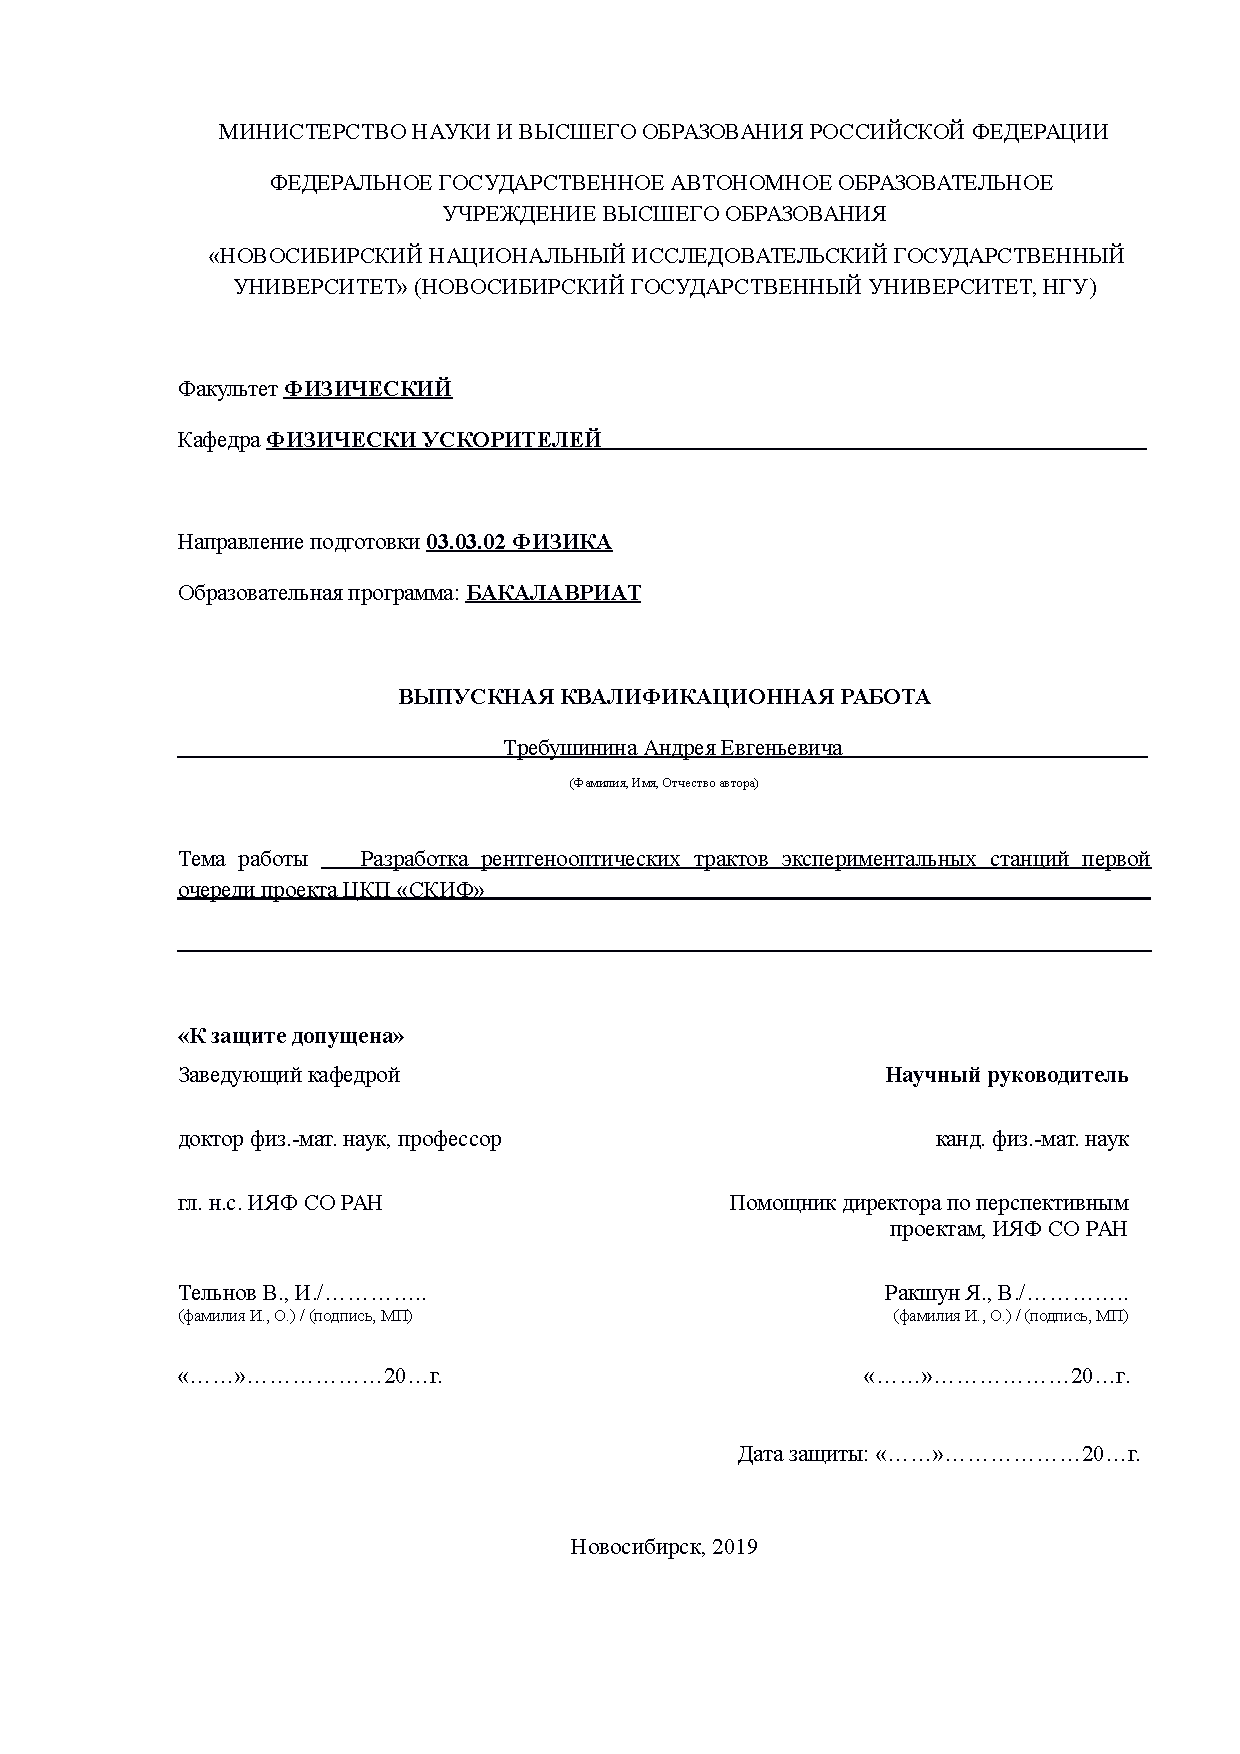
\includepdf{NSU/trebushi_title}    % Титульный лист от НГУ
%\chapter*{Аннотация}


% Оглавление (ГОСТ Р 7.0.11-2011, 5.2)
\pagenumbering{gobble}
\tableofcontents
\thispagestyle{empty}
        % Оглавление

\chapter{Ондуляторное излучение}
В этой части мы дадим вывод излучения релятивистского электрона в $r\omega$-пространстве, движущегося в синусоидальном магнитном поле. Вывод замечателен тем, что даёт результаты из первых принципов --- уравнений Максвелла, а точность используемых приближений можно наглядно проследить по ходу изложения. В выкладках мы следовали подходу разработанному в серии работ \cite{geloni2005paraxial}, \cite{geloni2007fourier}, \cite{geloni2015brightness }, \cite{geloni2006fourier}. В заключении главы, будет дан обзор на подход, который используется в симуляционном коде SRW \cite{chubar1998proceedings}, а также даны краткие описания других симуляционных кодов, которые активно используются в научном сообществе для расчёта синхротронного излечения. 
\section{Излучение релятивистского электрона в синусоидальном магнитном поле}
\subsection{Уравнение движения электрона в ондуляторе}
Выведем спектр излучения ондулятора. Вывод начнём с уравнения движение релятивистского электрона в магнитном поле.

\begin{equation}
	\vec{F} = e[\vec{v} \times \vec{B}],
\end{equation} 
где $e$ --- заряд электрона, а $\vec{v}$ и $\vec{B}$ --- скорость частицы и магнитное поле, соответственно. Уравнение можно переписать в виде:

\begin{equation}
	\label{eq:NewTown}
	\cfrac{d\vec{p}}{dt} = \cfrac{e}{\gamma m_e}[\vec{v} \times \vec{B}],
\end{equation}
где $\gamma$ --- лоренц фактор, появившийся из релятивистского импульса. Отложим ось $z$ вдоль направления релятивистского движения электрона и будем считать, магнитное поле в ондуляторе $B_0\cos(k_w z)$ направлено вдоль оси $y$, где $k_w$ связана с периодом ондулятора следующим образом $k_w = 2\pi/\lambda_w$. После этого уравнение~\ref{eq:NewTown} можно переписать в виде:

\begin{equation}
	\label{eq:eq_of_motion}
	\begin{cases}
		\cfrac{d^2 x}{dt^2} = - \cfrac{e B_0}{\gamma m_e}\cfrac{dz}{dt} \cos(k_w z)\\
		\cfrac{d^2 z}{dt^2} = \cfrac{e B_0}{\gamma m_e}\cfrac{dx}{dt} \cos(k_w z)
	\end{cases} 
\end{equation}
далее, один раз интегрируя первое уравнение системы с заменой $dz = \beta cdt$, где $\beta = \|\vec{v}\| /c$, можно получить: 

\begin{equation}
 	\label{eq:dx/dt}
	\cfrac{dx}{dt} = - \cfrac{eB_0}{\gamma m_ek_w} \sin(k_w z)
\end{equation}
Введём коэффициент ондуляторности --- $K = \cfrac{eB_0 \lambda_u}{2 \pi m_e c}$, который показывает угол отклонения траектории электрона от оси $z$. 

Подставляя получившийся результат~\ref{eq:dx/dt} во второе уравнение системы~\ref{eq:eq_of_motion} и интегрируя с пределами от $0$ до некоторого $z_0$, получим систему:

\begin{equation}
	\begin{cases}
	\label{eq:eq_of_motion_velocity}
		\cfrac{dx}{dt} = - \cfrac{Kc}{\gamma} \sin(k_w z)\\
		\cfrac{dz}{dt} = \beta c - \cfrac{K^2 c}{2 \gamma^2 \beta}\sin^2(k_w z)
	\end{cases} 
\end{equation}
Чтобы получить уравнение на траекторию частицы, ещё раз проинтегрируем оба уравнения и получим:

\begin{equation}
	\begin{cases}
	\label{eq:eq_of_motion_trej}
		x = \cfrac{Kc}{\gamma k_w \beta} \cos(k_w\overline{\beta}ct)\\
		z = \overline{\beta}ct + \cfrac{K^2}{8 \beta^2 \gamma^2 k_w}\sin(2k_w\overline{\beta}ct) 
	\end{cases} 
\end{equation}
Здесь мы ввели обозначение $\overline{\beta}$, которое определяется как $\overline{\beta}c = \beta c\bigg(1 - \cfrac{K^2}{4 \beta^2 \gamma^2}\bigg)$. Полученные решения мы будем использовать при интегрировании уравнений Максвелла.
%Из~\ref{eq:eq_of_motion_velocity} видно, что продольная скорость испытывает о осцилляции с удвоенной частотой...
\subsection{Решение уравнений Максвелла в прааксиальном приближении}
Вывод спектра излучения будем проводить в $r\omega$-пространстве. Начнём с уравнений Максвелла в вакууме:
\begin{equation}
	\begin{cases}
		\nabla \cdot \vec{E} = 4\pi \rho\\
		\nabla \cdot \vec{B} = 0\\
		[\nabla \times \vec{E}] = -\cfrac{1}{c} \cfrac{\partial\vec{B}}{\partial t}\\
		[\nabla \times \vec{B}] = \cfrac{4\pi}{c} \vec{j} + \cfrac{1}{c} \cfrac{\partial\vec{E}}{\partial t}
	\end{cases} 
\end{equation}
Из уравнений тривиально можно получить неоднородное волновое уравнение: 
\begin{equation}
	\label{eq:inhomo_wave_eq_xt}
	c^2 \nabla^2 \vec{E} - \pdv[2]{\vec{E}}{t} = 4\pi c^2 \nabla \rho + 4\pi \pdv{\vec{j}}{t}
\end{equation}
Это же уравнение перепишем в $r\omega$-пространстве, определив преобразование Фурье следующим образом:
\begin{equation}
	\label{eq:Fourier_wt}
	\begin{array}{lcl}
		\vec{\widetilde{E}}(r, \omega) = \displaystyle\int\limits_{-\infty}^{\infty} dt \vec{E}(r, t)\exp[i\omega t]\\
		\\
		\vec{E}(r, \omega) = \cfrac{1}{2\pi}\displaystyle\int\limits_{-\infty}^{\infty} d\omega \vec{\widetilde{E}}(r, t)\exp[-i\omega t]
	\end{array}
\end{equation}
Применив к уравнению~\ref{eq:inhomo_wave_eq_xt}, получим:
\begin{equation}
	\label{eq:inhomo_wave_eq_xw}
	\omega^2 \vec{\widetilde{E}} + c^2 \nabla^2 \vec{\widetilde{E}} = 4\pi c^2 \nabla  \widetilde{\rho} - 4i\pi\omega\vec{\widetilde{j}}
\end{equation}
Перепишем это уравнение в приближении медленно меняющейся амплитуды в сравнение с частотой осцилляций, что есть $\vec{\widetilde{E}} =  \vec{\overline{E}}\exp[i\omega z/c]$, в приближении $\cfrac{\partial |\vec{E}|}{\partial z} \ll \cfrac{\omega}{c}|\vec{E}|$. Где временная зависимость разложена до нулевого порядка малости, исходя из уравнения~\ref{eq:eq_of_motion_trej} получим:
\begin{equation}
	\label{eq:wave_slow_vary}
	c^2\bigg(\nabla^2 \vec{\widetilde{E}} + \cfrac{2i\omega}{c}\pdv{\vec{\widetilde{E}}}{z}\bigg)\exp[i\omega z/c] = 4\pi c^2 \nabla  \widetilde{\rho} - 4i\pi\omega\vec{\widetilde{j}}
\end{equation}
Для электрона движущегося в вакууме ток и плотность заряда выражается через дельта-функцию Дирака:

\begin{equation}
	\begin{array}{lcl}
		\rho(r,t) = -e\delta(\vec{r}- \vec{r'}(t)) = -\cfrac{e}{v_z(z)}\delta(\vec{r}_{\bot}- \vec{r'}_{\bot}(z))\delta(\cfrac{s(z)}{v} - t)\\
		\vec{j}(r,t) = \vec{v}\rho(r,t)	
	\end{array}
\end{equation} 
В $r\omega$-пространстве: 
\begin{equation}
	\begin{array}{lcl}
		\widetilde{\rho}(r,\omega) = -\cfrac{e}{v_z(z)}\delta(\vec{r}_{\bot}- \vec{r'}_{\bot}(z))\exp[\cfrac{iws(z)}{v}]\\
		\widetilde{\vec{j}}(r,\omega) = \vec{v}\widetilde{\rho}(r,\omega)	
	\end{array}
\end{equation} 
Подставим фурье-образы плотности тока и заряда в уравнение~\ref{eq:wave_slow_vary}:
\begin{equation}
	\label{eq:wave_eq}
	\begin{array}{lcl}
		\nabla^2 \vec{\widetilde{E}} + \cfrac{2i\omega}{c}\cfrac{\partial\vec{\widetilde{E}}}{\partial z} = 
		\cfrac{4\pi e}{v_z(z)} \exp[iw\bigg(\cfrac{s(z)}{v} - \cfrac{z}{c}\bigg)]
		\bigg(  
			\cfrac{i\omega}{c^2}\vec{v}(z)
			-\nabla\bigg) \delta(\vec{r}_{\bot} - \vec{r'}_{\bot}(z)) 
		
	\end{array}
\end{equation} 
Получившиеся уравнение является точным. Теперь мы можешь применить параксиальное приближение. 
\begin{equation}
	\label{eq:wave_slow_vary_parax}
	\begin{array}{lcl}
		\nabla_{\bot}^2 \vec{\widetilde{E}}_{\bot} + \cfrac{2i\omega}{c}\cfrac{\partial\vec{\widetilde{E}}_{\bot}}{\partial z} = 
		\cfrac{4\pi e}{v_z(z)} \exp[iw\bigg(\cfrac{s(z)}{v} - \cfrac{z}{c}\bigg)]\bigg(  
			\cfrac{i\omega}{c^2}\vec{v}_{\bot}(z) 
			-\nabla_{\bot}\bigg) \delta(\vec{r}_{\bot} - \vec{r'}_{\bot}(z)) 
	\end{array}
\end{equation} 
Перед нами неоднородное дифференциальное уравнение в частных производных, которое мы решим с помощью функции Грина. Для дифференциального оператора $\partial_t - k\nabla_{2D}^2$ функция Грина есть: $\cfrac{1}{4\pi kt}\exp[-\rho^2/4kt]$. В частности для уравнения~\ref{eq:wave_slow_vary_parax}
\begin{equation}
	\label{eq:Green_func}
	G(z_0 - z'; \vec{r}_{\bot 0} - \vec{r'}_{\bot}) = 
	- \cfrac{1}{4\pi (z_0 - z')}\exp[i\omega \cfrac{|\vec{r}_{\bot 0} - \vec{r'}_{\bot}|^2}{2c(z_0 - z')}]
\end{equation} 
Получим решение для функции распределения поля:

\begin{equation}
	\begin{array}{lcl}
		\vec{\widetilde{E}}_{\bot}(z_0,  \vec{r}_{\bot 0}, \omega) = -\cfrac{e}{c}  \displaystyle\int\limits_{-\infty}^{\infty}\int\limits_{-\infty}^{\infty} dz'd\vec{r'}\cfrac{1}{z_0 - z'}
		\bigg(\cfrac{i\omega}{c^2}\vec{v}_{\bot}(z')
		-\nabla'_{\bot}\bigg) \delta(\vec{r'}_{\bot} - \vec{r'}_{\bot}(z'))\times\\
		\exp[iw\bigg( \cfrac{|\vec{r}_{\bot 0} - \vec{r'}_{\bot}|^2}{2c(z_0 - z')} +\cfrac{s(z')}{v} - \cfrac{z'}{c} \bigg)]
	\end{array}	
\end{equation}
Проинтегрировав по $d\vec{r'}$ получим общее решение уравнения~\ref{eq:wave_eq} :
\begin{equation}
	\label{eq:field_in_parax_com}
	\begin{array}{lcl}
		\vec{\widetilde{E}}_{\bot}(z_0,  \vec{r}_{\bot 0}, \omega) = -\cfrac{i\omega e}{c^2}  \displaystyle\int\limits_{-\infty}^{\infty} dz'
		\cfrac{1}{z_0 - z'}
		\bigg(\cfrac{\vec{v}_{\bot}(z')}{c}
		- \cfrac{\vec{r}_{\bot 0} - \vec{r'}_{\bot}(z')}{(z_0 - z')}\bigg)\times\\
		\exp[iw\bigg(\cfrac{|\vec{r}_{\bot 0} - \vec{r'}_{\bot}(z')|^2}{2c(z_0 - z')} + \cfrac{s(z')}{v} - \cfrac{z'}{c} \bigg)].
	\end{array}	
\end{equation}
Итого, мы получили распределение электромагнитного поля в точке наблюдения $\vec{r}_0$, которое получит явный вид после интегрирования по траектории $\vec{r'}_{\bot}(z')$.

\subsection{Излучение планарного ондулятора}
В этой секции мы рассмотрим излучение планарного ондулятора, используя результаты~\ref{eq:field_in_parax_com} и~\ref{eq:eq_of_motion_trej}. Сперва проанализируем получившиеся распределение поля~\ref{eq:field_in_parax}: в случае ондулятора, член $(z_0 - z')^{-1}$ можно разложить около $z'$, что всегда верно для дальней зоны, так как размер ондулятора много меньше расстояния, с которого наблюдается излучения: $\lambda_w N \ll z_0$, где $N$ число периодов ондулятора.

Воспользовавшись решениями~\ref{eq:eq_of_motion_velocity} и~\ref{eq:eq_of_motion_trej} и помня $\vec{r}_{\bot 0}/z_0 = \vec{\theta}$, преобразуем уравнение~\ref{eq:field_in_parax_com} к виду:
\begin{equation}
	\label{eq:field_in_parax}
	\begin{array}{lcl}
		\vec{\widetilde{E}}_{\bot}(z_0,  \vec{r}_{\bot 0}, \omega) =
		\cfrac{i\omega e}{c^2z_0} \exp[i\cfrac{\omega \theta^2 z_0}{2c}]
	 	\displaystyle\int\limits_{-\lambda_w N/2}^{\lambda_w N/2} dz'\exp[i\Phi_T]
		\bigg(\cfrac{K}{\gamma}\sin(k_w z)\vec{e}_x + \vec{\theta}\bigg)
	\end{array}	
\end{equation}
Здесь мы отбросили члены первого и больших порядков малости по $1/z_0$. За $\Phi_T$ мы обозначили следующее выражение:
\begin{equation}
	\Phi_T = 
	\bigg(\cfrac{\omega}{2c\widetilde{\gamma}^2} + 
	\cfrac{\omega\vec{\theta}^2}{2c}\bigg)z' - 
	\cfrac{K^2}{8\gamma^2}\cfrac{\omega}{k_w c}\sin(2k_wz') - \cfrac{K{\theta_x}}{\gamma}\cfrac{\omega}{k_w c}\cos(k_w z'),
\end{equation}
а $\widetilde{\gamma} = \cfrac{\gamma}{\sqrt{1 + K^2/2}}$.\\

Пределы интегрирования ограничили длиной ондулятора от $-\lambda_w N/2$ до $\lambda_w N/2$, считая вклад в излучение ондулятора доминирующим над вкладами от остальных участков траектории. На этом шаге уже можно заметить, что излучение на оси будет линейно поляризованно. По ходу выкладок можно проследить, что это есть вклад токового члена из уравнения~\ref{eq:inhomo_wave_eq_xw}, вклад же плотности заряда или, как мы его назовём, градиентный член, даёт вариацию поляризации при наблюдении под некоторым углом $\theta$ к оси.
Перепишем~\ref{eq:field_in_parax} в следующе виде:
\begin{equation}
		\label{eq:field_in_parax_Bessel}
		\begin{array}{lcl}
			\vec{\widetilde{E}}_{\bot}(z_0,  \vec{r}_{\bot 0}, \omega) =
			\cfrac{i\omega e}{c^2z_0} \exp[i\cfrac{\omega \theta^2 z_0}{2c}]
			\displaystyle\sum_{m,n=-\infty}^{+\infty}
			J_m\bigg(-\cfrac{K^2}{8\gamma^2}\cfrac{\omega}{k_w c}\bigg)
			J_n\bigg(-\cfrac{K{\theta_x}}{\gamma}\cfrac{\omega}{k_w c}\bigg)\times\\
			\exp[\cfrac{i\pi n}{2}]
			\displaystyle\int\limits_{-\lambda_w N/2}^{\lambda_w N/2} dz'\exp[i(2m + n)k_wz']
			\bigg(\cfrac{K}{2i\gamma}\big(\exp[2ik_w z'] - 1\big)\vec{e_x} + \vec{\theta}\exp[ik_w z']\bigg)\times\\
			\exp[i\bigg(k_w \cfrac{\Delta\omega}{\omega_r} + 
			\cfrac{\omega\vec{\theta}^2}{2c}\bigg)z'],
		\end{array}	
\end{equation}
Где мы ввели $\omega = \omega_r + \Delta\omega$, $\omega_r = 2c\widetilde{\gamma}^2k_w$ и использовали формулу Якоби — Ангера:
\begin{equation}
	\begin{array}{lcl}
		\exp[iz\cos(\theta)] = 
		\displaystyle\sum\limits_{n =-\infty}^{\infty}
		i^n J_n(z)\exp[in\theta]\\	
		\exp[iz\sin(\theta)] = 
		\displaystyle\sum\limits_{n =-\infty}^{\infty}
		J_n(z)\exp[in\theta]
	\end{array}	
\end{equation}

До сих пор мы пользовались только одним приближением при решении уравнения Максвелла --- параксиальным приближением, теперь можем воспользоваться следующим параметром --- количеством периодов ондулятора $N$. Для этого обратим внимание на первое слагаемое в фазовом множителе под интегралом и заметим, что если $k_w \cfrac{\Delta\omega}{\omega_r} + 
\cfrac{\omega\vec{\theta}^2}{2c} \ll k_w$, то фаза меняется медленно на одном периоде и не занулит интеграл. Отметим, что для резонанса об слагаемых должны быть много меньше единицы, т.е. $\cfrac{\Delta\omega}{\omega_r} \ll 1$ и $\cfrac{\omega\vec{\theta}^2}{2c} \ll 1$, последнее соотношение даёт углы наблюдения вблизи резонанса: $\theta \ll \cfrac{1}{\widetilde{\gamma}}$. Теперь необходимо обратить внимание на аргументы функций Бесселя, а именно: 
\begin{equation}
	\begin{array}{lcl}
		u = -\cfrac{K^2}{8\gamma^2}\cfrac{\omega}{k_w c}\\
		v = -\cfrac{K{\theta_x}}{\gamma}\cfrac{\omega}{k_w c} = - \cfrac{K{\theta_x}}{\gamma}
		\bigg(1 + \cfrac{\Delta\omega}{\omega_r}\bigg)2\widetilde{\gamma}^2 \lesssim
		\cfrac{2K{\theta_x}\widetilde{\gamma}}{\sqrt{1 + K^2/2}} \lesssim \theta_x\widetilde{\gamma} \ll 1
	\end{array}	
\end{equation}
Зная, что $J_\alpha(x) \thicksim \displaystyle\sum\limits_{n =0}^{\infty} x^{2n + \alpha} $, видим, что вклад нулевого порядка по $\theta_x\widetilde{\gamma}$, т.е. $J_\alpha(x) \thicksim 1$, даёт только функция Бесселя с индексом $n = 0$. Здесь мы пока не учитываем градиентный член пропорциональный $\vec{\theta}$, таким образом из оставшихся фазовых множителей можно выписать условия на индекс $m$. Они определяются нулями в аргументах соответствующих фаз или $m = -1$ и $m = 0$, оба оставшихся члена пропорциональны $\cfrac{K}{\gamma}$. 

Теперь вернёмся к градиентному члену, вклад от которого занулиться при усреднении по длине ондулятора при $n = 0$, этот вклад даст ненулевой вклад при $n = 1 - 2m$, таким образом в ход пойдут следующие члены разложения $J_m(v)$. Однако, помня интересующий нас диапазон углов, члены разложения будут порядка $\theta_x v^m$, очевидно, что их вклады пренебрежимо малы, и вклад токового члена $\vec{e}_x$ будет доминирующем. Учитывая вышесказанные приближения, перепишем~\ref{eq:field_in_parax_Bessel}
\begin{equation}
	\label{eq:field_dist_in_integral}
	\begin{array}{lcl}
		\vec{\widetilde{E}}_{\bot}(z_0,  \vec{r}_{\bot 0}, \omega) =
		\cfrac{\omega e}{2c^2z_0}\cfrac{K}{\gamma}\exp[i\cfrac{\omega \theta^2 z_0}{2c}]
		\bigg(J_1(v) - J_0(v)\bigg)\vec{e}_x\times\\
		\\
		\displaystyle\int\limits_{-\lambda_w N/2}^{\lambda_w N/2} dz'
		\exp[i\bigg(k_w \cfrac{\Delta\omega}{\omega_r} + 
		\cfrac{\omega\vec{\theta}^2}{2c}\bigg)z'],
	\end{array}	
\end{equation}
Интеграл легко берётся:
\begin{equation}
	\label{eq:field_dist_nonNorm}
	\begin{array}{lcl}
		\vec{\widetilde{E}}_{\bot}(z_0,  \vec{r}_{\bot 0}, \omega) =
		\cfrac{\omega eL}{c^2z_0}\cfrac{K}{\gamma}A_{JJ}\exp[i\cfrac{\omega \theta^2 z_0}{2c}]
		\sinc \bigg[\bigg(k_w \cfrac{\Delta\omega}{\omega_r} + 
		\cfrac{\omega\vec{\theta}^2}{2c}\bigg)L/2 \bigg ]\vec{e}_x ,
	\end{array}	
\end{equation}
где введено обозначение: $A_{JJ} = J_1(v) - J_0(v)$. В итоге мы получили распределение поля в $r\omega$-пространстве. 

В следующем параграфе мы займёмся выводном влияния конечности эмиттанса на распределение излучения, чтобы облегчить выкладки мы введём нормализованные единицы.
\begin{equation}
	\label{eq:norm_units}
	\begin{array}{lcl}
		\hat{E}_{\bot} = \cfrac{c^2z_0\gamma \widetilde{E}_{\bot}}{e\omega KLA_{JJ}}\\
		\\
		\hat{\theta} = \theta\sqrt{\cfrac{\omega L}{c}}\\
		\\
		\hat{z} = \cfrac{z}{L} ,
	\end{array}	
\end{equation}
а также, 
\begin{equation}
	\hat{C} = CL = 2\pi N\cfrac{\Delta\omega}{\omega_r}
\end{equation}
Теперь уравнения~\ref{eq:field_dist_nonNorm} и~\ref{eq:field_dist_in_integral} могут быть переписаны в нормализованных единицах.
\begin{equation}
	\label{eq:field_dist_in_integral}
	\begin{array}{lcl}
		\hat{E}_{\bot} = e^{i\Phi}
		\displaystyle\int\limits_{-1/2}^{1/2} dz'
		\exp[i\bigg(\hat{C} + 
		\cfrac{\hat{\theta}^2}{2}\bigg)z'],
	\end{array}	
\end{equation}

\begin{equation}
	\label{eq:field_dist_Norm}
	\begin{array}{lcl}
		\hat{E}_{\bot} = e^{i\Phi}
		\sinc\bigg(\cfrac{\hat{C}}{2} + 
		\cfrac{\hat{\theta}^2}{4}\bigg),
	\end{array}	
\end{equation}
\begin{figure}
	\centering  
	\begin{minipage}{0.49\textwidth}
		\centering
		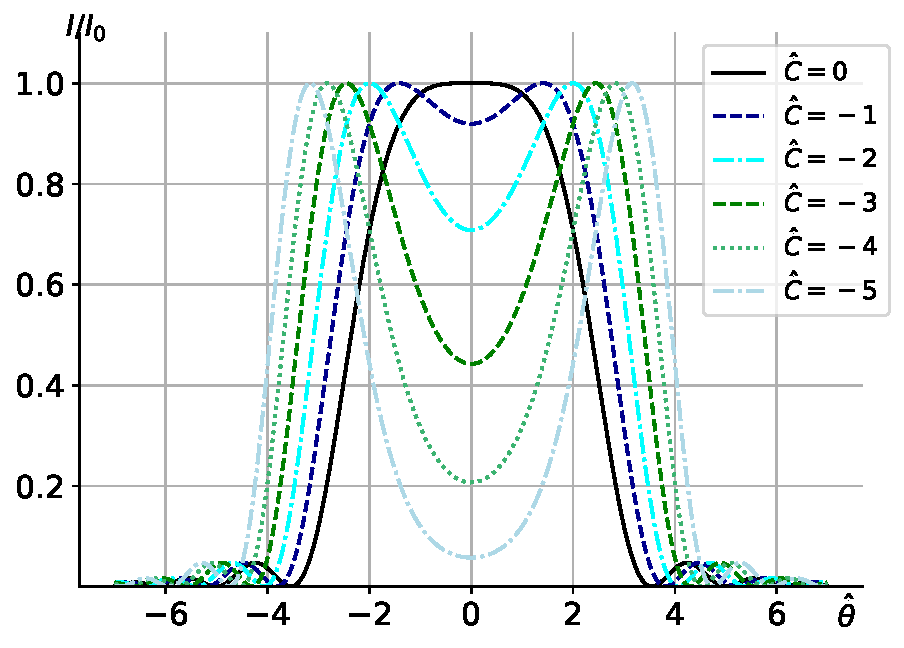
\includegraphics[width=\textwidth]{pic/angleC_neg.pdf}
		\caption{Угловое распределение поля при отрицательной сдвижке частоты}
		\label{fig:angle_dist_C_neg}
	\end{minipage}\hfill
	\begin{minipage}{0.49\textwidth}
		\centering
		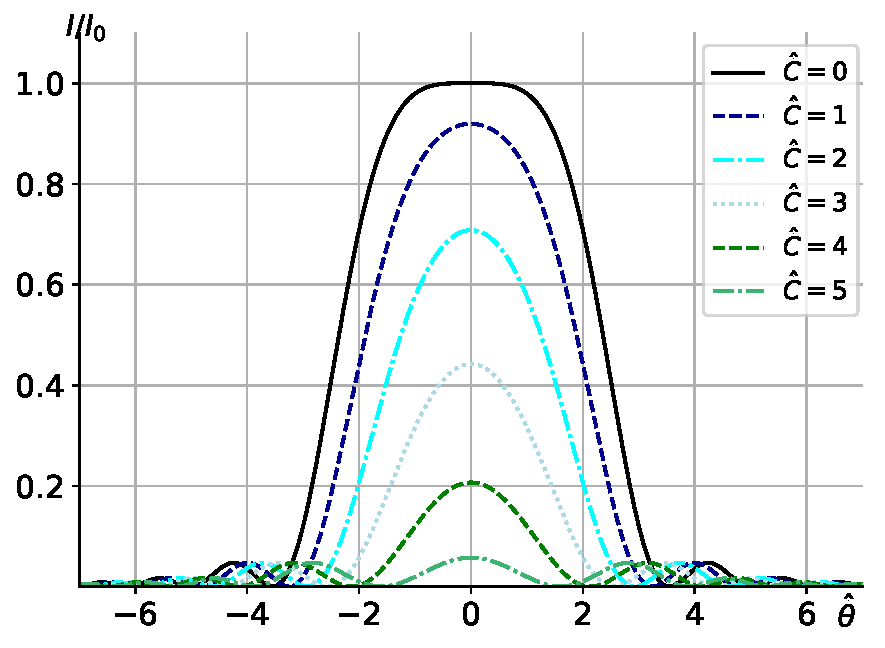
\includegraphics[width=\textwidth]{pic/angleC_pos.pdf}
		\caption{Угловое распределение поля при положительной сдвижке частоты}
		\label{fig:angle_dist_C_pos}
	\end{minipage}    
\end{figure}
На рис.~\ref{fig:angle_dist_C_neg} и рис.~\ref{fig:angle_dist_C_pos} изображены угловые распределения излучения. Их структуру можно понять из рисунка~\ref{fig:traj}. Конструктивная интерференция наблюдается на оси, где есть максимум интерференционной картины на резонансной частоте. Если произвести отрицательную сдвижку по частоте, то выполнение условия конструктивной интерференции: $n \lambda_{ph} = s_{ph} - \lambda_u \cos\theta$ будет наблюдаться при ненулевых углах наблюдения, и обратно, при положительной сдвижке частоты, интенсивность быстро падает, условие резонанса не может выполниться при меньших длинах волн на ненулевых углах, потому что в набег фазы на каждом периоде ондулятора, не укладывается целое число длин волн соответствующей гармоники излучения. Говорят, что электрон на каждом периоде ондулятора интерферирует сам с собой. Естественно, говорят о интерференции излучения, которое на оси обгоняет электрон на одну длину волны (или болеешее число волн, т.е. 1, 2, 3 и т.д.). На следующем периоде ондулятора, электрон снова излучает в фазе с излучённой на прошлом периоде волной. Важной характеристикой в приложениях является проинтегрированный по углам $\hat{\theta}$ спектр излучения, см. рис.~\ref{fig:spec_integrate_angle}. В некотором смысле, у спектра появляется широкий хвост. Форма спектра и единицы измерения для некоторой конкретной задачи должны обсуждаться отдельно.  
\begin{figure}[htbp]
	\centering
	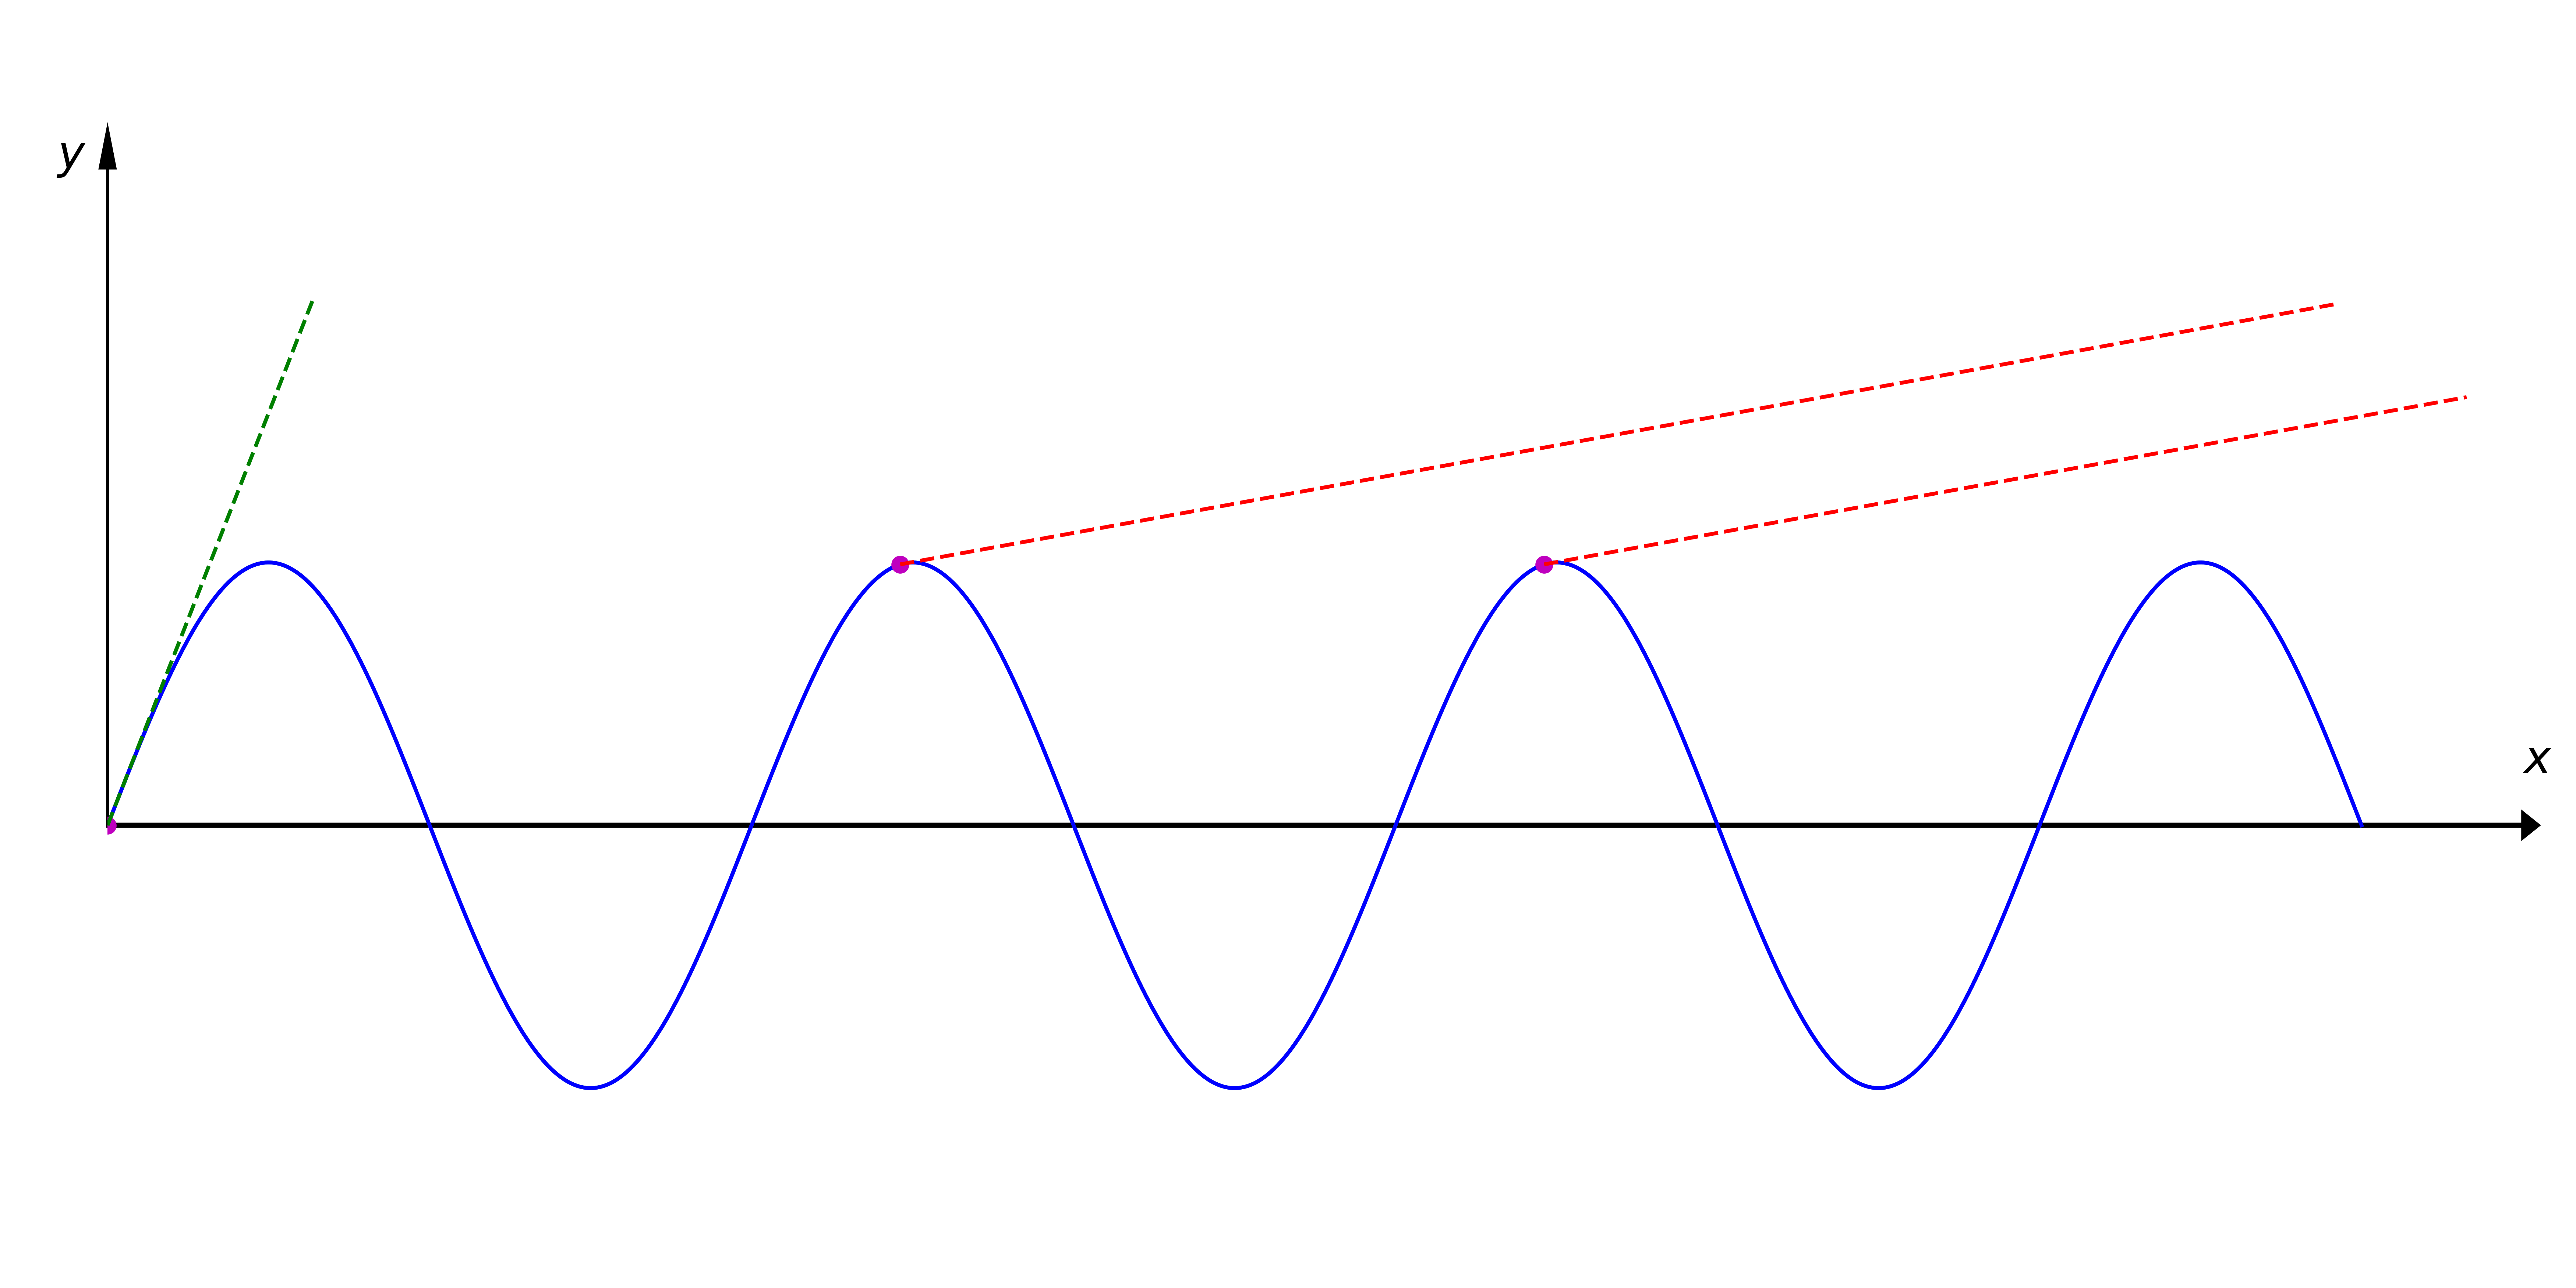
\includegraphics[width=.99\textwidth]{{pic/traj}.pdf}
	\caption{Ондулятор как интерференционное устройство} 
	\label{fig:traj}
\end{figure}

\begin{figure}[h!]
	\centering
	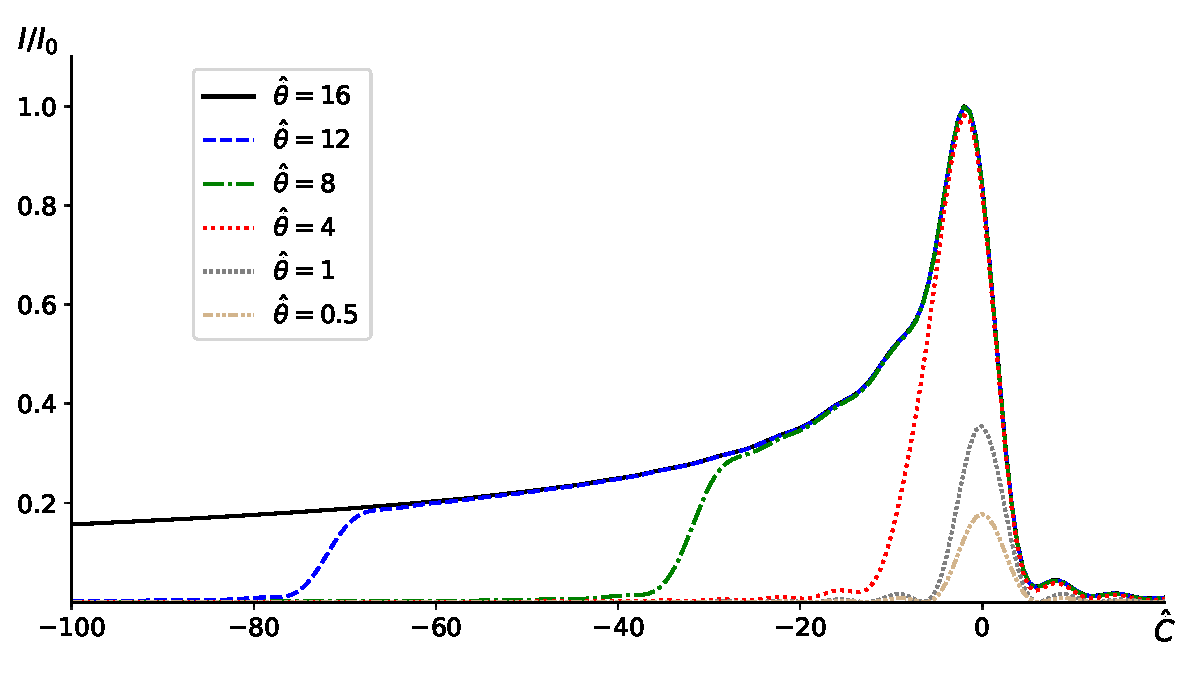
\includegraphics[width=.99\textwidth]{{pic/spec_integ_ang}.pdf}
	\caption{Проинтегрированный по углам спектр излучения. За $\hat{\theta}$ в легенде обозначены пределы интегрирования по углам} 
	\label{fig:spec_integrate_angle}
\end{figure}

\section{Излучение высших гармоник}
\subsection{Амплитудный спектр высших гармоник ондуляторного излучения в зависимости от параметра ондуляторности}
В этом разделе мы дадим описание свойств излучения высших гармоник. Начнём с объяснения амплитудного спектра ондуляторного излучения. Понимание данного вопроса необходимо в виду того, что выбор конкретных параметров ондулятора, обычно говорят о параметре ондуляторности $K$, чрезвычайно важен для приложений. Выбор этого параметра напрямую влияет на состав спектра излучения и его амплитудное распределение. Следуя выкладками~\ref{eq:field_dist_nonNorm}, где было введено обозначение $A_{JJ}$, и общей формуле для произвольной гармоники из \cite{wiedemann2015particle} можно написать:
\begin{equation}
	\label{eq:A_JJ}
	A_{JJ}(K) = \cfrac{n^2 K^2}{(1 + K^2/2)^2} \bigg[ J_{\frac{1}{2}(k-1)}\bigg(\cfrac{nK^2}{4 + 2K^2}\bigg) - J_{\frac{1}{2}(k+1)}\bigg(\cfrac{nK^2}{4 + 2K^2}\bigg)\bigg]^2,
\end{equation}
\begin{figure}[h]
	\centering 
	\begin{minipage}{0.99\textwidth}
		\centering
		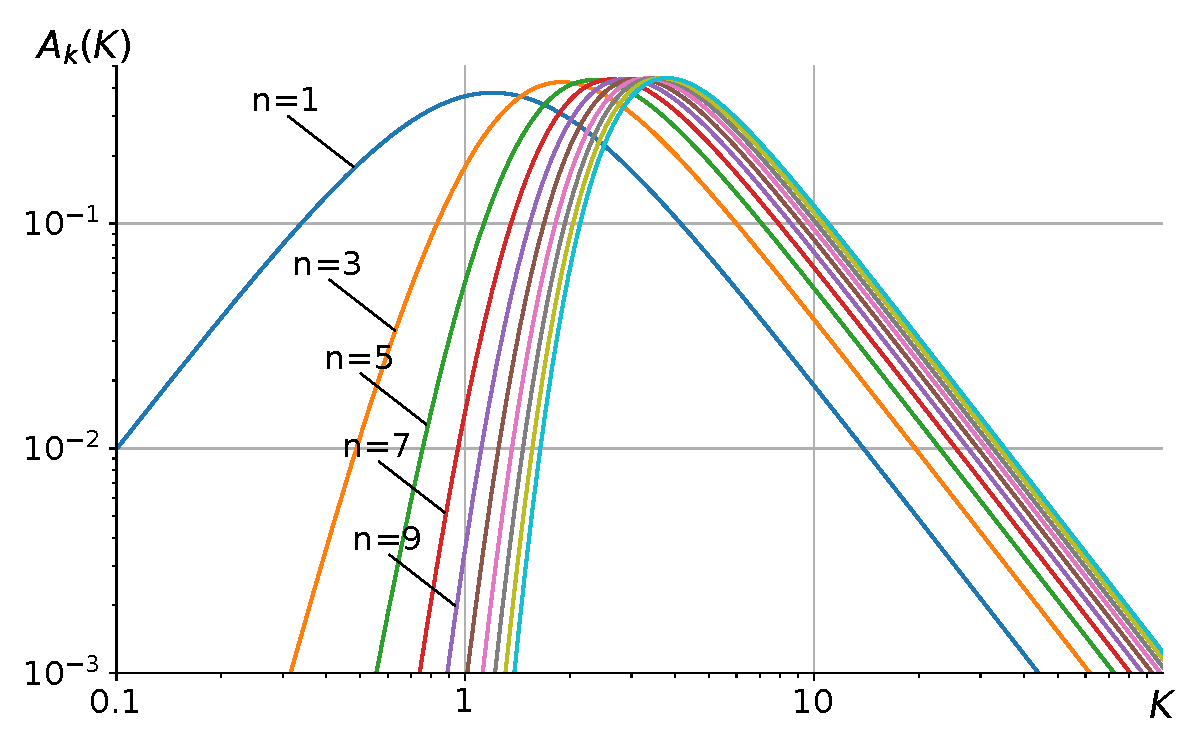
\includegraphics[width=.79\textwidth]{{pic/A_K}.pdf}
		\caption{Амплитудный спектр гармоник в зависимости от параметра ондуляторности $K$} 
		\label{fig:A_K}
	\end{minipage}
\end{figure}

Графическое представление этой формулы в зависимости от параметра $K$ показано на рис.~\ref{fig:A_K}. Спектр наглядно показывает зависимость амплитуд гармоник от параметра ондуляторности. На ондуляторах, где планируется работать на низших гармониках, преимущественно выбираются малые $K < 2$, если же стоят задачи, где используются более высокие гармоники, то параметр $K$ выбирают в районе $2 - 2,5$.

На рис.~\ref{fig:spec_und_1-1} и рис.~\ref{fig:spec_und_1-2} представлены примеры спектров ондуляторного излучения электронного пучка с бесконечно малым эмиттансом. Рисунки наглядно поясняют соображения изложенные выше по амплитудному составу ондуляторного спектра. Уже при при $K = 2,5$ максимум амплитуды приходиться на $7$-ую гармонику.
\begin{figure}[ht!]
	\begin{minipage}{0.49\textwidth}
		\centering
		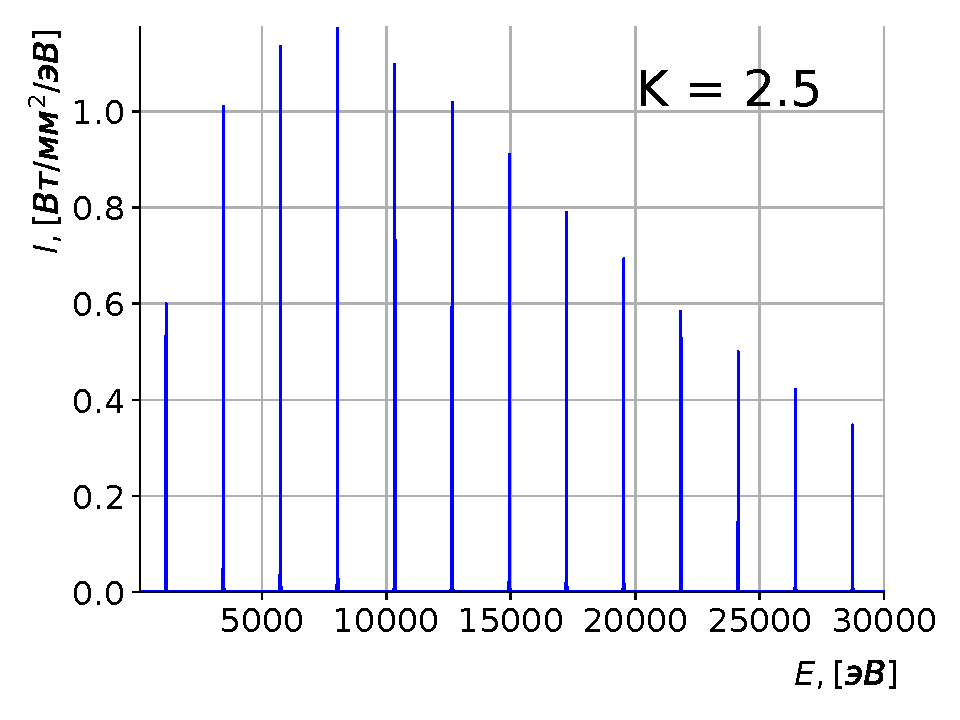
\includegraphics[width=\textwidth]{pic/spec_und_1-1.pdf}
		\caption{Спектр ондулятора с ондуляторностью $K = 2,5$}
		\label{fig:spec_und_1-1}
	\end{minipage}
	\begin{minipage}{0.49\textwidth}
		\centering
		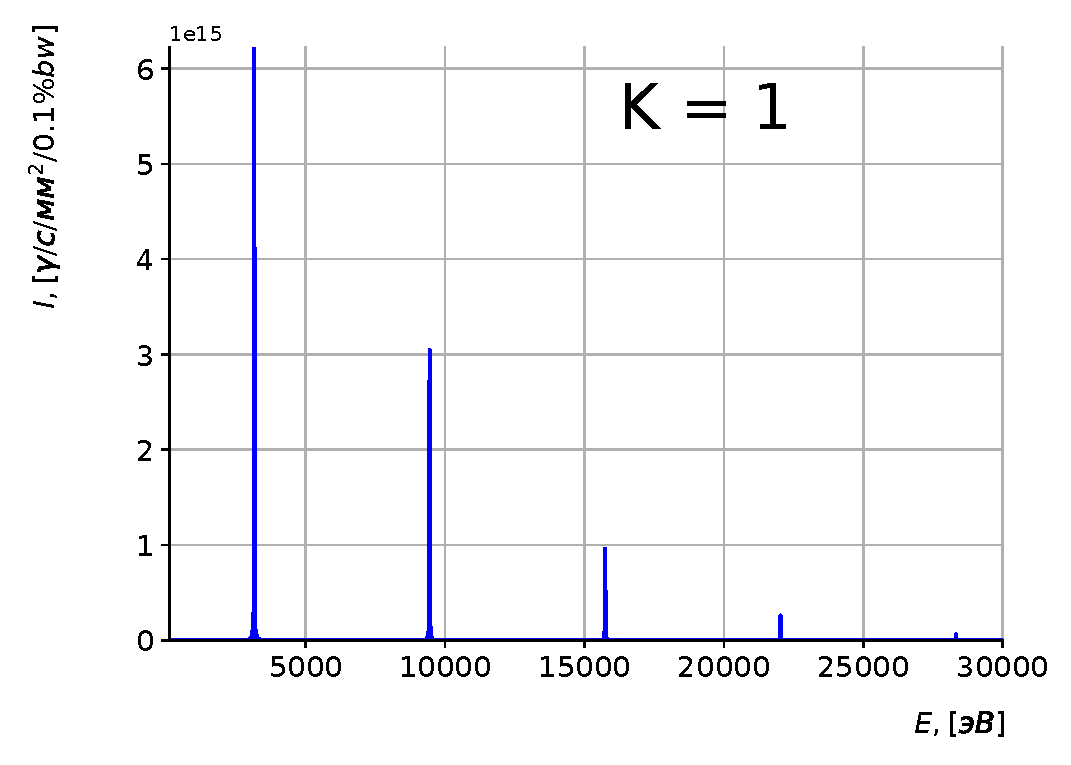
\includegraphics[width=\textwidth]{pic/spec_und_1-2.pdf}
		\caption{Спектр ондулятора с ондуляторностью $K = 1$}
		\label{fig:spec_und_1-2}
	\end{minipage}    
\end{figure}

\section{Заключение}










\chapter{Элементы фурье оптики}
В этой главе мы предложим наглядный подход к решению задачи о распространение волнового фронта в пустом пространстве, его прохождении через систему линзу. Приведённые результаты напрямую могут быть использованы в программном коде. Распределение поля в начальный момент времени будем считать гауссовским, однако, как будет видно из изложения, подход может быть использован для произвольного распределения поля. В наших выкладкам мы в полной мере следуем подходу \cite{serkez2013grating} и \cite{serkez2015design}, полное изложение фурье оптики и статистической оптики можно найти в замечательных книгах \cite{goodman2015statistical}, \cite{goodman2005introduction}. В конце главы будет приведёт пример учебного кода \cite{my_github} для распространения волнового фронта через оптическую систему, написанный автором в рамках одного из университетских курсов.

\section{Распространение света в пустом пространстве}
Наши рассуждения мы начнём с волнового уравнения в пустом пространстве, т.е. $\vec{j} = 0, \rho = 0$. 
\begin{equation}
	\pdv[2]{\vec{E}}{t} + c^2 \nabla^2 \vec{E} = 0
\end{equation}
В  $r\omega$-пространстве уравнение приобретает знакомый вид уравнения Гельмгольца, где $k_0 = \omega/c$.

\begin{equation}
	k_0^2\vec{\widetilde{E}} + \nabla^2 \vec{\widetilde{E}} = 0
\end{equation}
Совершив фурье-преобразование в $k$-пространство по координатам $x,y$, которое определим схожим образом с~\ref{eq:Fourier_wt}:

\begin{equation}
	\label{eq:Fourier_rk}
	\begin{array}{lcl}
		\vec{\widehat{E}}(\vec{k}, \omega) = \displaystyle\int\limits_{-\infty}^{\infty}\int\limits_{-\infty}^{\infty} dxdy \vec{E}(\vec{r}, t)\exp[ik_xx + ik_xx]\\
		\\
		\vec{E}(\vec{r}, \omega) = \cfrac{1}{4\pi^2}\displaystyle\int\limits_{-\infty}^{\infty}\int\limits_{-\infty}^{\infty} dk_xdk_y \vec{\widehat{E}}(\vec{k}, t)\exp[-ik_xx - ik_xx],
	\end{array}
\end{equation}
получим: 
\begin{equation}
	k_0^2\Big(1 - \cfrac{k^2_x}{k^2_0} - \cfrac{k^2_y}{k^2_0} \Big)\vec{\widehat{E}} + \dv[2]{\vec{\widehat{E}}}{z} = 0
\end{equation}
Теперь можно напрямую можно получить решение этого обыкновенного дифференциального уравнения:
\begin{equation}
	\label{eq:sol}
	\vec{\widehat{E}}(\omega, k_x, k_y, z) = \vec{\widehat{E}}(\omega, k_x, k_y, 0)\exp[ik_0z\sqrt{1 - \frac{k^2_x}{k^2_0} - \frac{k^2_y}{k^2_0}} ]
\end{equation}
На основе уравнения~\ref{eq:sol} введём функцию отклика среды:

\begin{equation}
	\begin{array}{lcl}
	H(k_x, k_y, z) = \cfrac{\vec{\widehat{E}}(\omega, k_x, k_y, z)}{\vec{\widehat{E}}(\omega, k_x, k_y, 0)} = \exp[ik_0z\sqrt{1 - \cfrac{k^2_x}{k^2_0} - \cfrac{k^2_y}{k^2_0}} ]
	\\
	\\
	H(k_x, k_y, z) \approxeq \exp[k_0z]\exp[-\cfrac{iz}{2k_0}(k^2_x + k^2_y)]
	\end{array}
\end{equation}
Видно, чтобы получить распределение электромагнитного поля на некотором расстоянии $z$, необходимо совершить обратное преобразование Фурье в $xy$-пространство. Таким образом решение волнового уравнения сводиться к трём относительно простым операциям: первое, --- перевод начального распределения в $k_xk_y$-пространство, далее домножение получившегося распределения на функцию отклика среды, в нашем случае пустое пространство, и последний шаг, --- обратное преобразование Фурье. Из вывода видно,что мы не накладывали никаких ограничений на начальное распределение поля, кроме, быть может, естественных ограничений, накладываемых на оригинал преобразованием Фурье.

\section{Действие тонкой линзы на волновой фронт}
В этом параграфе мы построим элементарную оптическую систему, состоящую из пустого промежутка, --- $d_1$, тонкой линзы с оптической силой, --- $1/f$ и ещё одного пустого промежутка до плоскости изображения. Действие тонкой линзы мы представим как домножение комплексной амплитуды поля на следующее выражение: 
\begin{equation}
	T_f(x, y) = \exp[-\cfrac{ik_0}{2f}(x^2 + y^2)]
\end{equation}
Для предметности обсуждения определим начальное распределение гауссовым пучком: 

\begin{equation}
	\overline{E}(x, y, 0) = A\exp[-\cfrac{x^2 + y^2}{w^2_0}]
\end{equation}
После преобразование Фурье в $k_xk_y$-пространстве мы получим:

\begin{equation}
	\hat{E}(k_x, k_y, 0) = A\pi w^2_0\exp[-\cfrac{w^2_0}{4}(k_x^2 + k_y^2)]
\end{equation}
После домножения этого распределения поля в $k_xk_y$-пространстве на функцию отклика пустого промежутка, получим
\begin{equation}
	\label{eq:after_lens}
	\begin{array}{lcl}
	\hat{E}(k_x, k_y, z) = \hat{E}(k_x, k_y, z)H(k_x, k_y, z) 
	\\
	\\
	= A\pi w^2_0\exp[-\cfrac{w^2_0}{4}(k_x^2 + k_y^2)]\exp[k_0z]\exp[-\cfrac{iz}{2k_0}(k^2_x + k^2_y)]
	\\
	\\
	= A\pi w^2_0\exp[k_0z]\exp[-\cfrac{iq}{2k_0}(k^2_x + k^2_y)], 
	\end{array}
\end{equation}
здесь мы ввели $q = z - iz_R$, где $z_R = \cfrac{k_0w^2_0}{2}$. После перехода обратно в $xy$-пространство, получим: 
\begin{equation}
	\overline{E}(x, y, z) = \cfrac{iAk_0w^2_0}{2q}\exp[k_0z]\exp[-i\cfrac{k_0}{2q}(x^2 + y^2)],
\end{equation}
Теперь можно воспользоваться выражением для тонкой линзы и получить:
\begin{equation}
	\begin{array}{lcl}
	\overline{E}_{l}(x, y, z) = T_f(x, y)\overline{E}(x, y, z) = 
	\\
	\\
	\cfrac{iAk_0w^2_0}{2q}\exp[k_0z]\exp[-i\cfrac{k_0}{2q}(x^2 + y^2)]\exp[-\cfrac{ik_0}{2f}(x^2 + y^2)]
	\\
	\\
	\cfrac{iAk_0w^2_0}{2q}\exp[k_0z]\exp[-i\cfrac{k_0}{2q_l}(x^2 + y^2)],
	\end{array}
\end{equation}
где $\cfrac{1}{q_l} = \cfrac{1}{q} \; - \; \cfrac{1}{f}$. \\

Теперь можно подвести итог: после распространения волнового фронта на расстояние $d_1$ параметр $q$ преобразуется:
\begin{equation}
	q(d_1) = q(0) + d_1, 
\end{equation}
далее на него действует линза: 
\begin{equation}
	\cfrac{1}{q_l} = \cfrac{1}{q(0) + d_1} - \cfrac{1}{f},
\end{equation}
и ещё один пустой промежуток, до места, где волновой фронт опять будет плоским: 
\begin{equation}
	q(d_1 + d_2) = q_l + d_2, 
\end{equation}
Условие того, что волновой фронт плоский мы сформулируем так, что $q(d_1 + d_2) = -i\cfrac{k_0w^2_2}{2}$, что легко проверятся подстановкой в~\ref{eq:after_lens}. Получим уравнение: 
\begin{equation}
	-i\cfrac{k_0w^2_2}{2} = q_l + d_2, 
\end{equation}
где, приравниванием мнимых частей, получим: 
\begin{equation}
	w^2_2 = \cfrac{f^2w^2_1}{(f - d_1)^2 + (k_0w^2_1/2)^2}
\end{equation}
то же для реальных частей: 
\begin{equation}
	d_2 = f + f^2\cfrac{(d_1 - f)}{(d_1 - f)^2 + (k_0w^2_1/2)^2}
\end{equation}
Из последнего уравнения видно, что если положить перетяжку гауссового пучка раной нулю, то выражение переходит в соотношение геометрической оптики.

В приведённой главе мы дали краткий путь того, как можно очень эффективно и относительно просто использовать Фурье оптику для написания симуляционных кодов при проектировании оптических систем. В качестве примера, для заинтересованных читателей на веб-странице (веб-страница) приведёт код простой оптической системы, который в полной мере используют результаты вышеприведённого параграфа. Код был написан автором данной рукописи рамках курса <<Основы вычислительной физики>>, который читается на физическом факультете НГУ. Дальнейшие комментарии к коду можно найти в репозитории указанной по ссылке.

\chapter{Краткий обзор дифракции на кристаллах}
В это главе мы кратко дадим основные результаты кинетической и динамической теории дифракции. Основные кристаллы используемы на синхротронных источниках третьего и четвёртого поколений - это $Si$ (кремний), $C$ (алмаз) и реже $Ge$ (германий), в виду свой кубической кристаллический решётки, эти кристаллы относительно просты для анализа. Для нас важны такие свойства кристаллов, как способность преобразовать относительно широкой спектр излучения ондулятора, в излучение с относительной монохроматичностью до $\Delta E/ E \sim 10^{-4}$, а также поглощательные способности кристаллов, что в значительной степени снижает тепловые нагрузки на оптические элементы.
\section{Симметричное брэгговское отражение от идеально кристалла}
Длины волн, которые отвечают резонансу при отражении падающего под углом $\theta$ к плоскости кристалла излучения, даётся законом Брэгга:  
%пропорциональный $\gamma / nN$, где $n$ --- номер гармоники излучения, $N$ --- число периодов ондулятора, а $\gamma$ --- гамма фактор релятивистского электрона
\begin{equation}
	m\lambda = 2d\sin\theta,
\end{equation}
где $d$ --- расстояние между плоскостями от которых происходит отражение, а $m$ --- некоторое положительно целое число. Основной результат, который мы будем использовать, это кривая Дарвина, которая определяет угловой акцептанс излучения. Динамическая и кинематическая теории дифракции дают конечную ширину в, которую кристалл может принять излучение, а также некоторый сдвиг, относительно предполагаемого брэгговского угла. На рис.~\ref{fig:bragg_R} показаны характерные кривые отражение. По ним видно, что чем больше энергия подающего пучка излучения, тем уже кривая и ближе к даваемому законом брэгга углу. При расчёте кристаллов монохроматоров этот факт необходимо учитывать, так как излучение не попавшее в акцептанс кристалла будет поглощаться и выделять в нем тепло. 
\section{Поглощательные способности кристаллов}
Одним из полезных применение кристаллов в рентгеновском диапазоне есть их фильтрующая способность, отрезать низкие энергии, в особенности для алмазных кристаллов, которые, по мимо всего, имеют хорошую теплопроводность, что способствуют быстрому теплоотводу. На рис.~\ref{fig:bragg_T} представлена кривая поглощения 100 мкм кристалла алмаза. Подобные кристаллы устанавливают перед первыми оптическими элементами, что в значительной степени снижает тепловые нагрузки, подавлением низших гармоник.
\begin{figure}
	\centering  
	\begin{minipage}{0.49\textwidth}
		\centering
		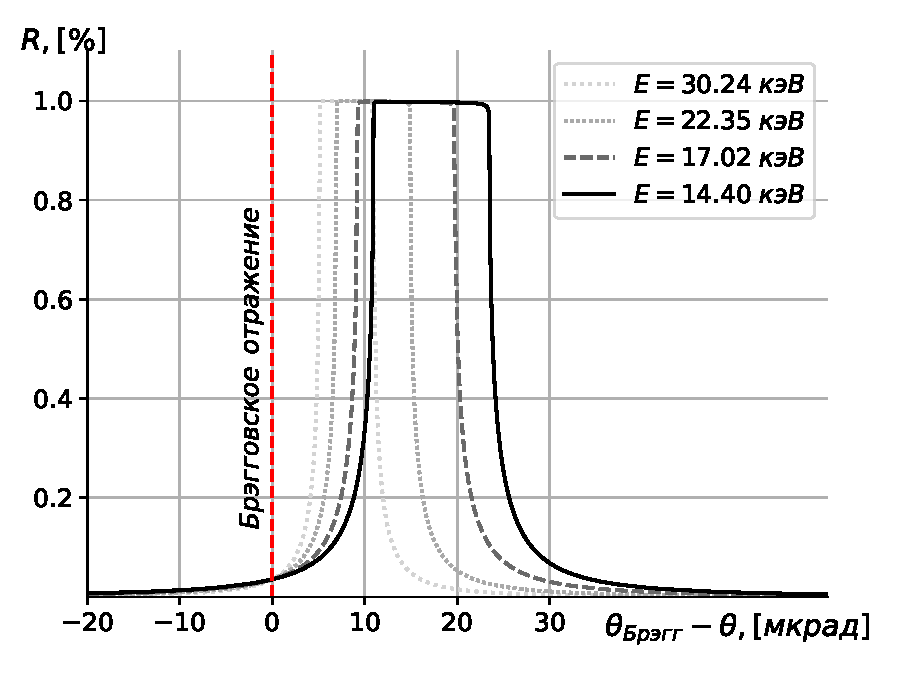
\includegraphics[width=\textwidth]{pic/bragg_R.pdf}
		\caption{}
		\label{fig:bragg_R}
	\end{minipage}\hfill
	\begin{minipage}{0.49\textwidth}
		\centering
		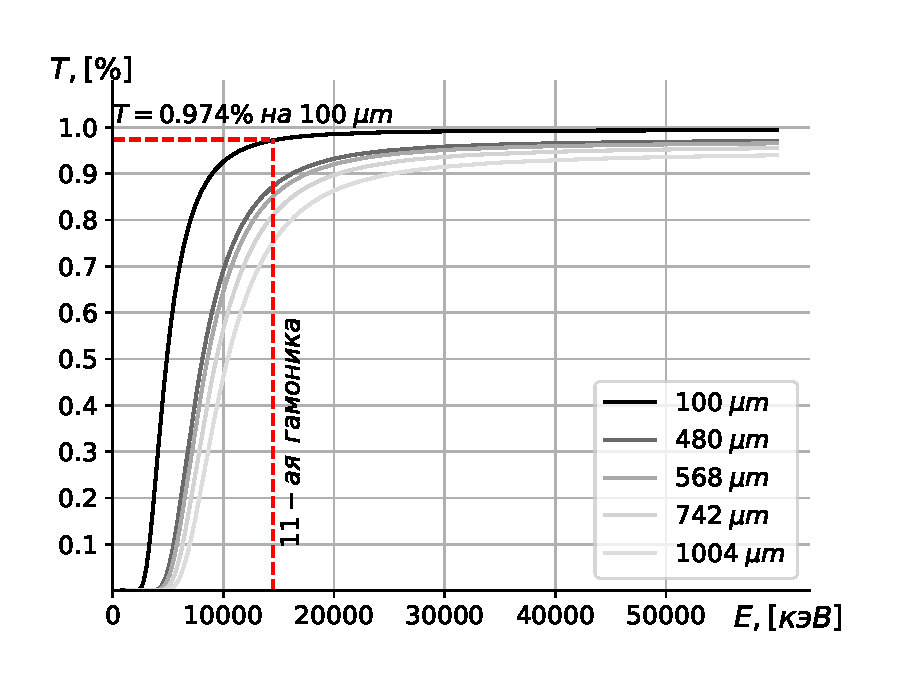
\includegraphics[width=\textwidth]{pic/bragg_T.pdf}
		\caption{}
		\label{fig:bragg_T}
	\end{minipage}    
\end{figure}

\chapter{Проектирование рентгенооптических трактов Сибирского Кольцевого Источника Фонтов}

\section{Введение}
В данной главе мы рассмотрим схемы рентгенооптических трактов (станций) первой очереди Центра Коллективного Пользования СКИФ: от источников высокого энергетических фотонов --- вставных устройств до деталей оптических компотен на билайне, --- фильтров, монохроматоров, рентгеновских зеркал и линз. В этой главе, будут обсуждаться станции: 1-1 --- <<Микрофокус>>, 1-2 --- <<Структурная диагностика>>, 1-4 --- <<XAFS-спектроскопия и магнитный дихроизм>>.  
\begin{table}[h!]
	\caption{Параметры накопительного кольца и электронного пучка в ондуляторном пустом промежутке}
	\centering
	\label{table:ebeam}
	\begin{tabular}{c|c|c|c}
		\hline\hline
		%\toprule
		\rule{0pt}{3ex}   $\sigma_x, [m]$ & $\sigma_{x'}, [rad]$ & $\sigma_y, [m]$     & $\sigma_{y'}, [rad]$ \\ \hline
		\rule{0pt}{3ex}   $33.0 \times 10^{-6}$  & $2.65 \times 10^{-6}$  &  $8.6 \times 10^{-7}$ & $5.0 \times 10^{-7}$   \\
		\hline	\hline
		\rule{0pt}{3ex}   $\Delta E / E$ & $\beta_x,[m]$ & $\beta_y,[m]$   & $I,[mA]$\\ \hline
		\rule{0pt}{3ex}	 $8.6 \times 10^{-4}$ & $12.49$ & $1.99$ & $400$ \\ \hline\hline
		%\toprule
	\end{tabular}
	\vspace{4pt} 
\end{table}

На всех указанных станциях будут использоваться сверхпроводящие ондуляторы разработки и производства ИЯФ СО РАН, см., например, \cite{bragin2018short} и \cite{gluskin2019superconducting}. Всё ондуляторы будут вводиться в пустой промежуток с геометрическими и угловыми размерами электронного пучка и бета функциями указанными в таблице~\ref{table:ebeam}. 

\section{Станция 1-1 --- <<Микрофокус>>}
\subsection{Вставное устройство}
Станция имеет вставное устройство с параметрами указанными в таб.~\ref{table:und1-1}. Выбора такого типа ондулятора объясняется тем, что на станции предполагается работать на довольно высоких гармониках, поэтому, согласно амплитудному спектру на рис~\ref{eq:A_JJ}, необходимо как можно далее сдвинуть максимум спектрального потока в сторону более высоких гармоник. 
\begin{table}[h!]
	\caption{Параметры ондулятора для станции 1-1}
	\centering
	\begin{tabular}{c|c|c|c}
		\hline\hline
		\rule{0pt}{3ex}$\mathnormal{B(K), [T]}$   & $\mathnormal{L, [m]}$ & $\mathnormal{d, [mm]}$ &  Рабочие Гармоники 1-1       \\ \hline
		\rule{0pt}{3ex}$1.36(2.29)$  & $2.3$    & $18$      & $11, 13, 17, 23$\\
		\hline\hline
	\end{tabular}
	\label{table:und1-1}
\end{table}
На рис.~\ref{fig:log_spec_1-1} представлен спектр используемого ондулятора через конечную апертуру, видно, что рабочие гармоники подавлены на порядок по сравнению с фундаментальной гармоникой.
\begin{figure}[h]
	\centering
	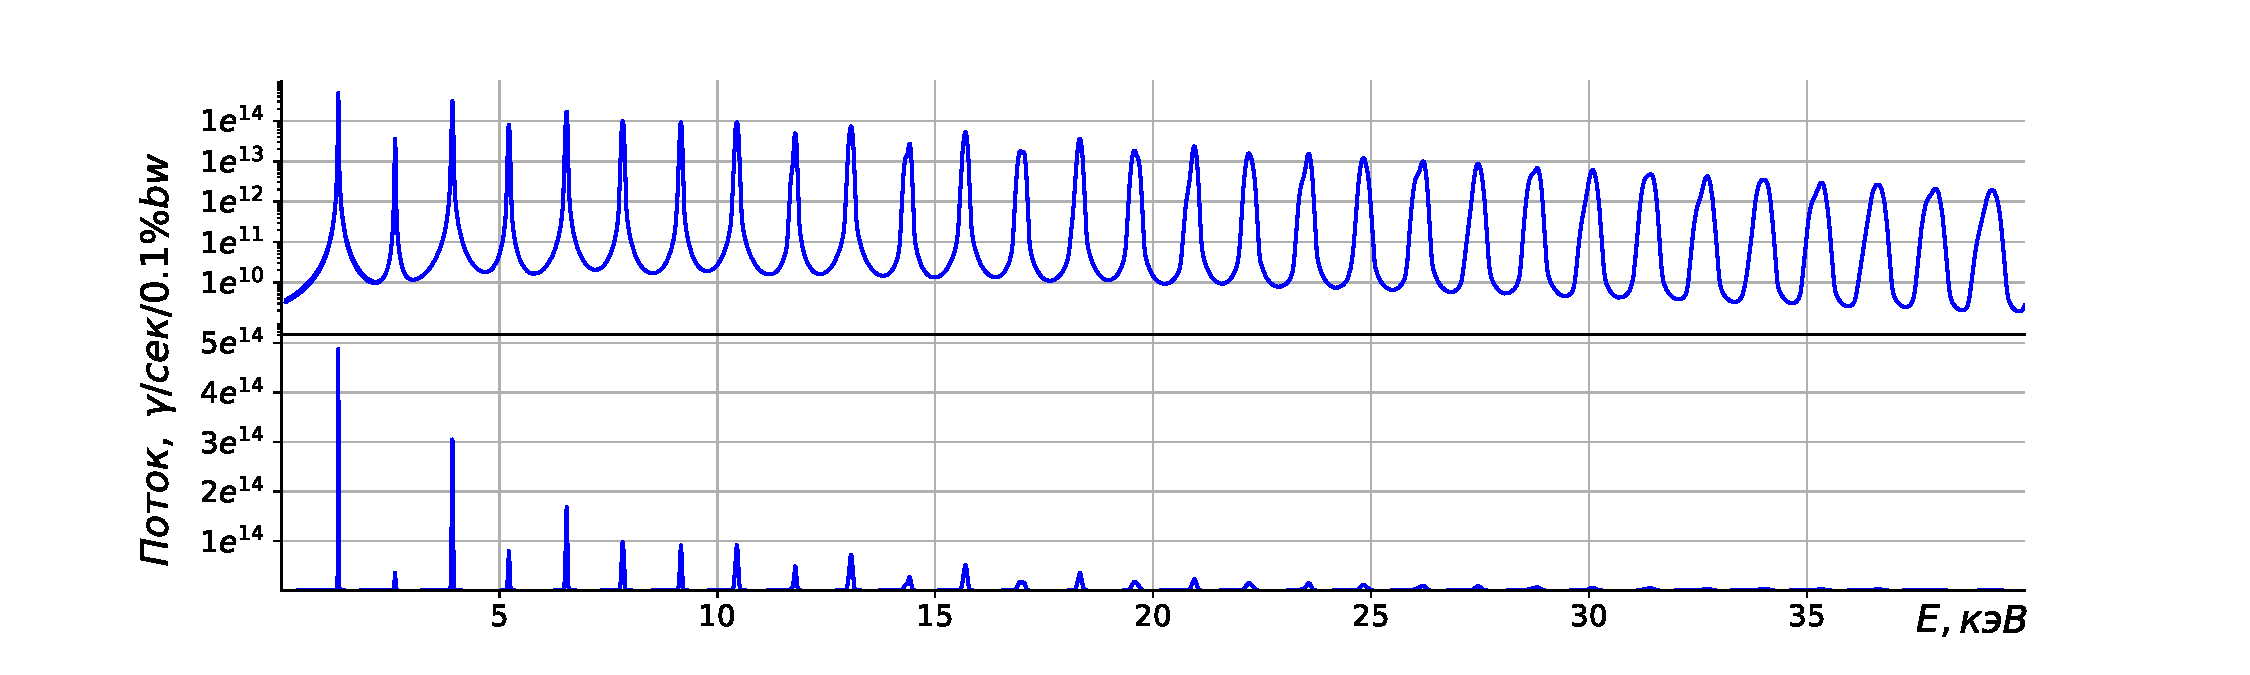
\includegraphics[width=\textwidth]{pic/log_spec_1-1.pdf}
	\caption{Спектр с ондулятора с $K = 2,29$ через апертуру $0,4 \; \textup{мм}$ в логарифмическом масштабе (сверху) и в линейном (снизу) посчитанный в SPECTRA с учётом конечности эмиттанса и энергетического разброса}
	\label{fig:log_spec_1-1}
\end{figure}

\subsection{Оптика станции 1-1}
Первостепенной задачей по расчёту оптики на рассматриваемой станции являлась оценка тепловых нагрузок на первые оптические элементы. На рис.~\ref{fig:OptScheme_1-1} представлена оптическая схема станции в первом приближении без фокусирующих линз. После прохождения пучком апертуры, которая является угловым фильтром, излучение проходит алмазное окно, толщина которого $100 \; \textup{мкм}$ из расчёта $\approx 3 \%$ поглощения на первой рабочей гармонике. Алмазные кристаллы являются хорошими фильтрами низких энергий. Основная тепловая нагрузка с первых гармоник снимается входным алмазным окном.
\begin{figure}[h!]
	\centering  
	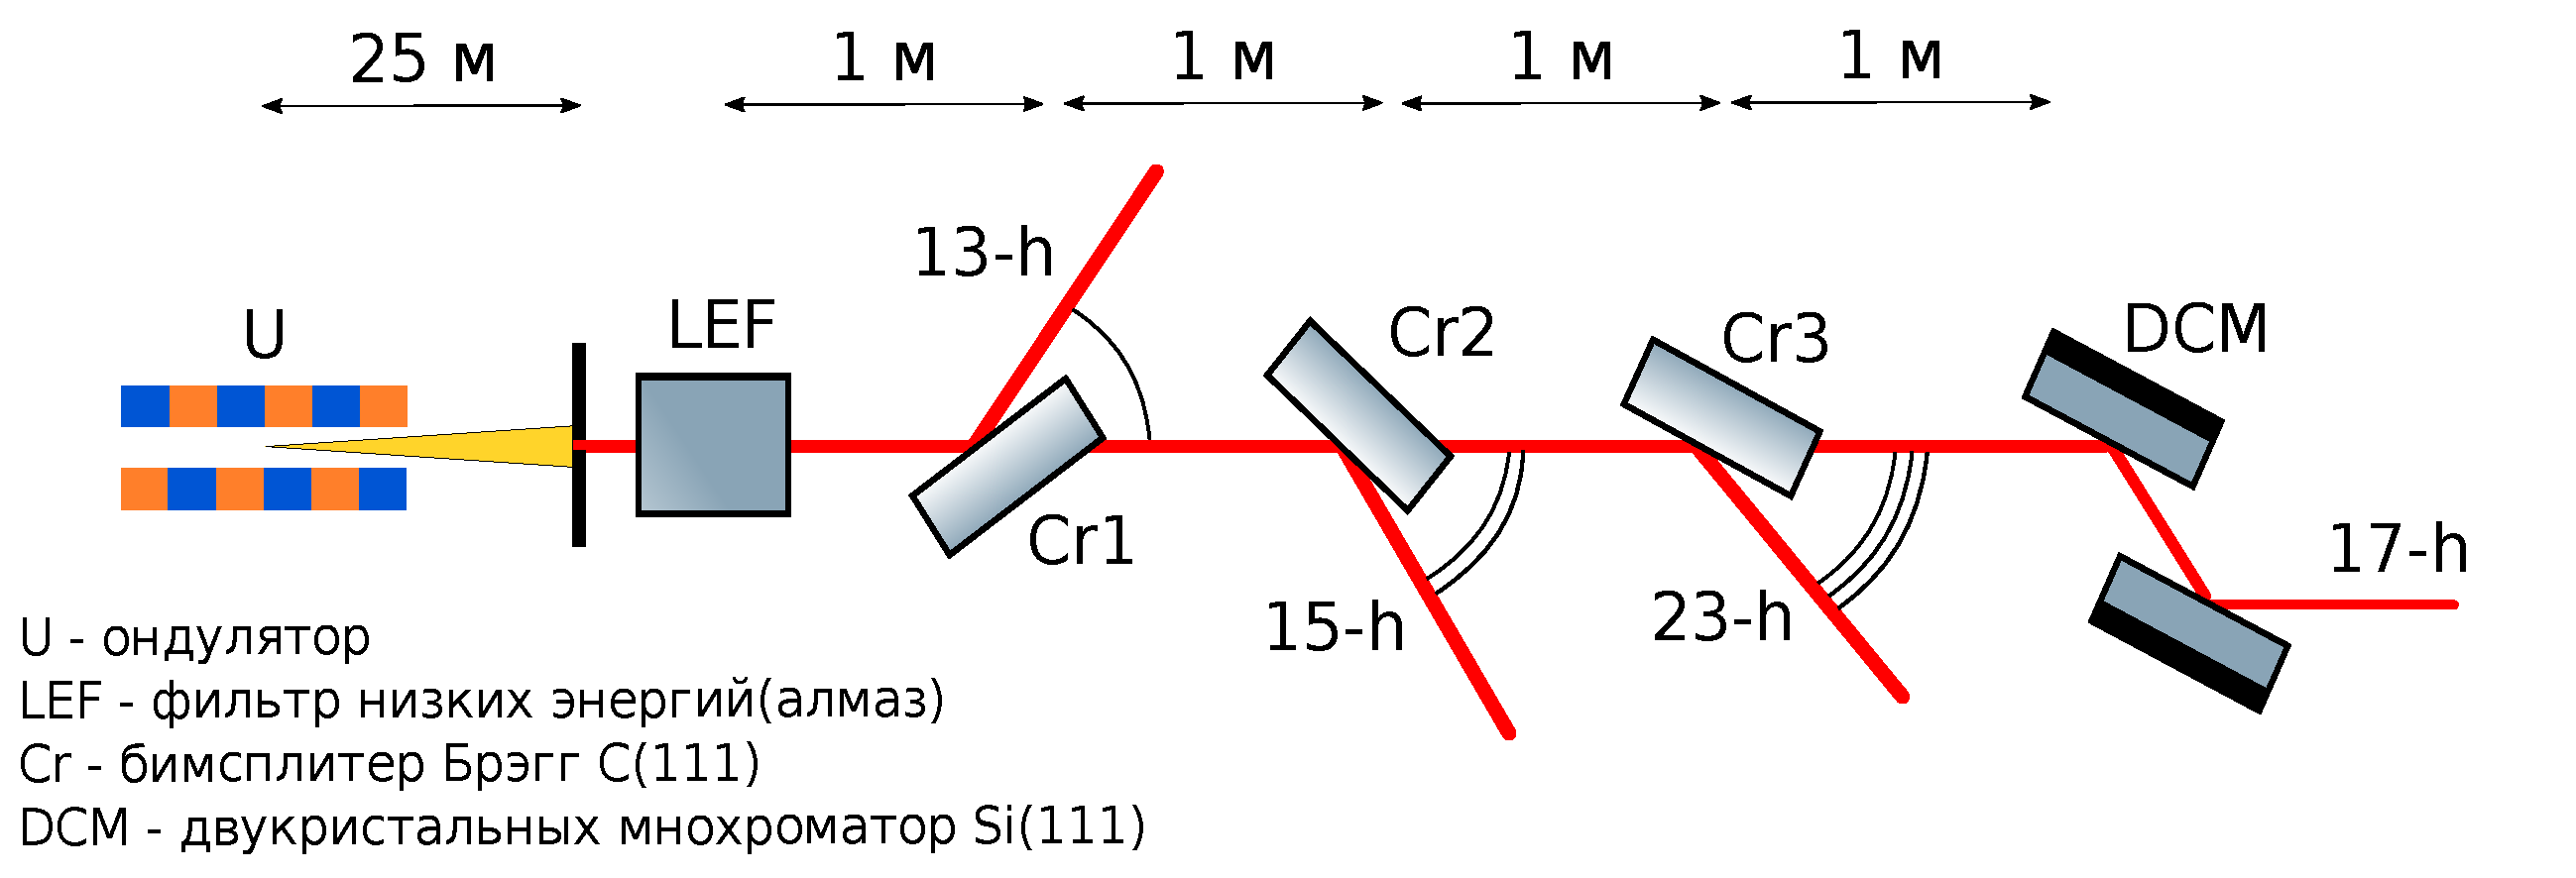
\includegraphics[width=\textwidth]{pic/OptScheme_1-1.pdf}
	\caption{Оптическая схема станции 1-1}
	\label{fig:OptScheme_1-1}  
\end{figure}
После алмазного окна излучение разделяется алмазными $C(111)$ монохроматорами на рабочие подстанции, прямой пучок падает на кремниевый $Si(111)$ двукристальный монохроматор. Поглощённые удельные мощности на каждом из представленных оптических элементах можно найти на рис.~\ref{fig:full_spec_1-1}.
\begin{figure}[h!]
	\centering
	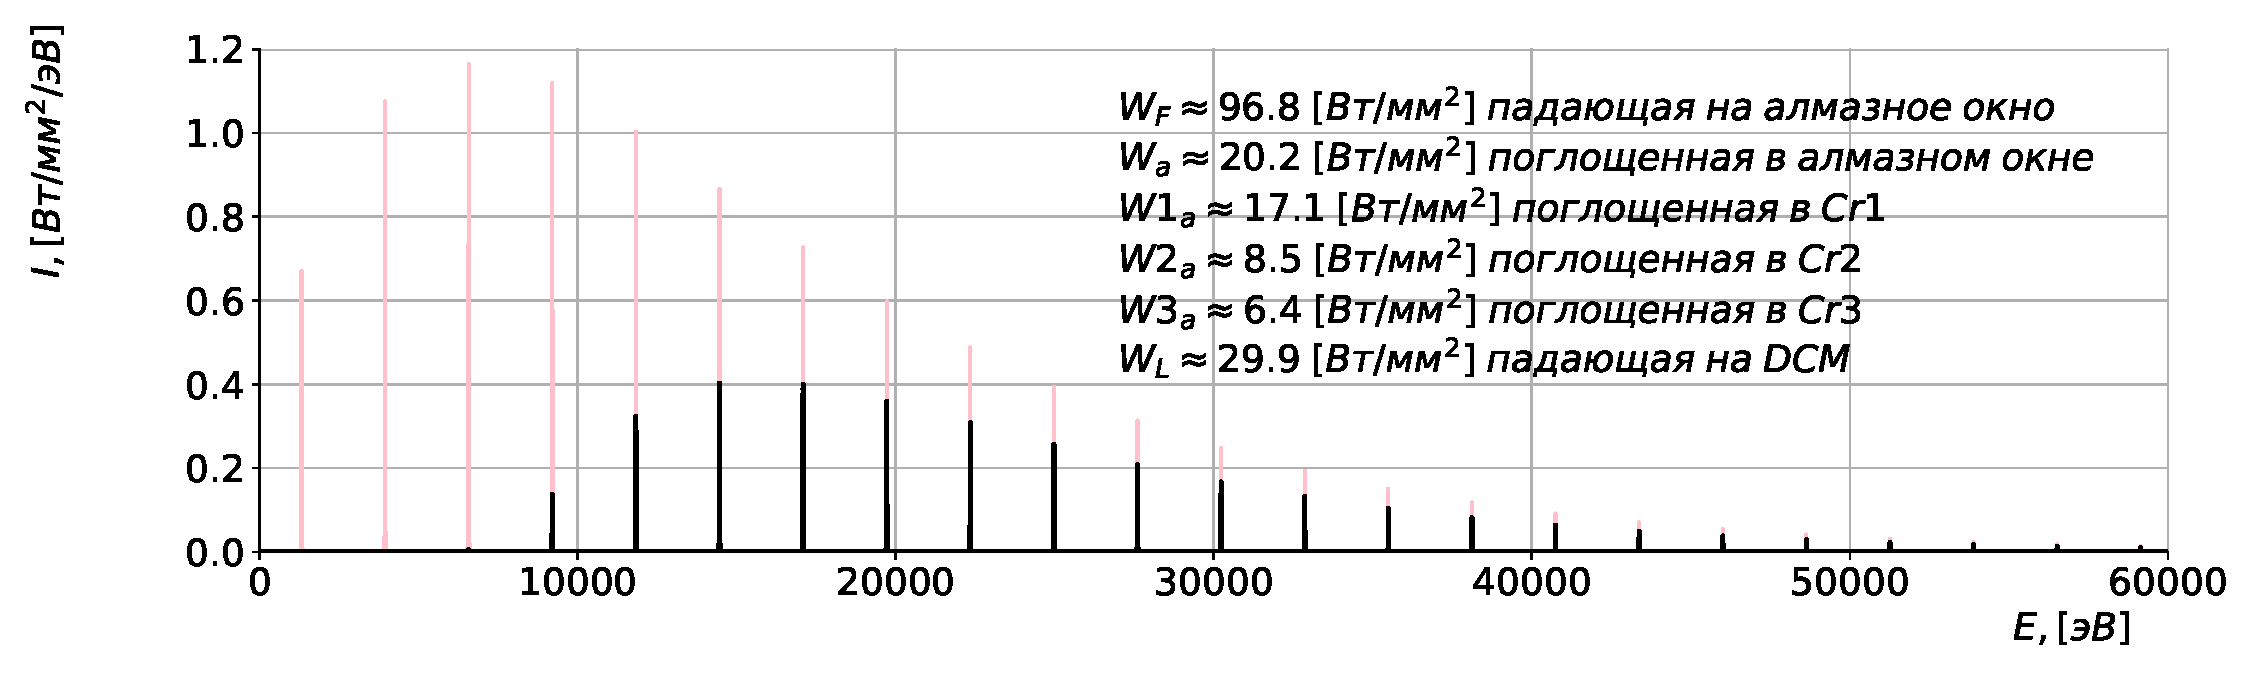
\includegraphics[width=\textwidth]{pic/full_spec_1-1.pdf}
	\caption{Спектр электронного пучка с нулевым эмиттансом падающий на алмазное окно --- розовый цвет, излучение падающее на двукристалльный монохроматор --- чёрный цвет}
	\label{fig:full_spec_1-1}   
\end{figure}
%Полезно сравнить расчёты связанные с полной падающей мощность на первый оптический элемент с одним из результатов встроенной функции в SRW по расчёту полной мощности, результаты этих расчётов приведены на рис.~\ref{fig:power_dens_1-1}. Необходимо отметить, что  эти расчёты~\ref{fig:full_spec_1-1} и рис.~\ref{fig:power_dens_1-1} независимы и совпадают, а незначительное отличие заключается лишь в том, что интегрирование на рис.~\ref{fig:full_spec_1-1} велось не по полному спектру, а лишь до энергии $60 \; \textup{кэВ}$, что не может привести ошибкам в расчётах, так как были не учтены фотоны с энергиями больше $60 \; \textup{кэВ}$, однако они являются прозрачными для большинства оптических элементов и не вносят значительного вклада в тепловые нагрузки.

Итого, результаты расчётов: 
\DTLloaddb
[
noheader,
keys={},
headers={
	\shortstack{$n_{harm}$},
	\shortstack{$\sigma_x, [mm]$},
	\shortstack{$\sigma_y, [mm]$},
	\shortstack{$\sigma_x, [\mu rad]$},
	\shortstack{$\sigma_y, [\mu rad]$}}
]
{RMS_before1-1}{tabl_1-1/RMS_before1-1.csv}
\begin{table}[h!]
	\caption{Сечение пучка на входе в первую апертуру (25 м)}
	\sisetup{
		parse-numbers   = false,
		table-number-alignment = right,
		table-figures-integer = 4,
		table-figures-decimal = 4,
		input-decimal-markers = .
	}
	\renewcommand*\dtlrealalign{S}
	\centering
	\DTLdisplaydb{RMS_before1-1}
	\label{table:size_obeam}
\end{table}

	\DTLloaddb
[
noheader,
keys={},
headers={
	\shortstack{$n_{harm}$},
	\shortstack{$\theta_{cr}, grad$},
	\shortstack{$d_{eff}, \mu m$},
	\shortstack{$S_{proj}, mm$}}
]
{Cr_angles1-1}{tabl_1-1/Cr_angles1-1.csv}
\begin{table}[h!]
	\caption{Номер гармоники, ориентация кристалла, эффективная толщина алмазного монохроматора, проекция пучка(горизонтальная) }
	\sisetup{
		parse-numbers   = false,
		table-number-alignment = right,
		table-figures-integer = 4,
		table-figures-decimal = 4,
		input-decimal-markers = .
	}
	\renewcommand*\dtlrealalign{S}
	\centering
	\DTLdisplaydb{Cr_angles1-1}
	\label{table:stable}
\end{table}

\DTLloaddb
[
noheader,
keys={},
headers={
	\shortstack{$n_{harm}$},
	\shortstack{$\sigma_x, [mm]$},
	\shortstack{$\sigma_y, [mm]$},
	\shortstack{$\sigma_x, [\mu rad]$},
	\shortstack{$\sigma_y, [\mu rad]$}}
]
{RMS_after1-1}{tabl_1-1/RMS_after1-1.csv}
\begin{table}[h!]
	\caption{Сечение пучка после монохроматоров}
	\sisetup{
		parse-numbers   = false,
		table-number-alignment = right,
		table-figures-integer = 4,
		table-figures-decimal = 4,
		input-decimal-markers = .
	}
	\renewcommand*\dtlrealalign{S}
	\centering
	\DTLdisplaydb{RMS_after1-1}
	\label{table:size_obeam_after}
\end{table}

\DTLloaddb
[
noheader,
keys={},
headers={
	\shortstack{$n_{harm}$},
	\shortstack{$E, eV$},
	\shortstack{$\lambda, [nm]$},
	\shortstack{$ph/s$},
	\shortstack{$ph/s/0.1\%$},
	\shortstack{$\Delta E / E$}}
]
{ph_beam_par_after_cr1-1}{tabl_1-1/ph_beam_par_after_cr1-1.csv}
\begin{table}[h!]
	\caption{Потоки фотонов после соответствующих монохроматоров}
	\sisetup{
		parse-numbers   = false,
		table-number-alignment = right,
		table-figures-integer = 4,
		table-figures-decimal = 4,
		input-decimal-markers = .
	}
	\renewcommand*\dtlrealalign{S}
	\centering
	\DTLdisplaydb{ph_beam_par_after_cr1-1}
\end{table}
\newpage

\section{Станция 1-2 --- <<Структурная диагностика>>}

\subsection{Вставное устройство}
На станции 1-2 используется сверхпроводящий ондулятор с параметром ондуляторности $K = 1.54$. На станции, в отличии от 1-1, предполагается работать на более низких гармониках, этим объясняется выбор указанного параметра $K$, амплитудный спектр смещён в сторону фундаментальной гармоники. В таблице~\ref{table:und1-2} приведены основные характеристики используемого ондулятора, а на рис.~\ref{fig:log_spec_1-2} показан спектр этого ондулятора через конечную апертуру.
\begin{table}[h!]
	\caption{Параметры ондулятора для станции 1-2}
	\centering
	\begin{tabular}{c|c|c|c}
		\hline\hline
		\rule{0pt}{3ex}$\mathnormal{B(K), [T]}$   & $\mathnormal{L, [m]}$ & $\mathnormal{d, [mm]}$ &  Рабочие Гармоники 1-2       \\ \hline
		\rule{0pt}{3ex}$1.06(1.54)$    			  & $2$                   & $15.6$      		   & $5, 7, 9, 13$\\
		\hline\hline
	\end{tabular}
	\label{table:und1-2}
\end{table}

\begin{figure}[h!]
	\centering
	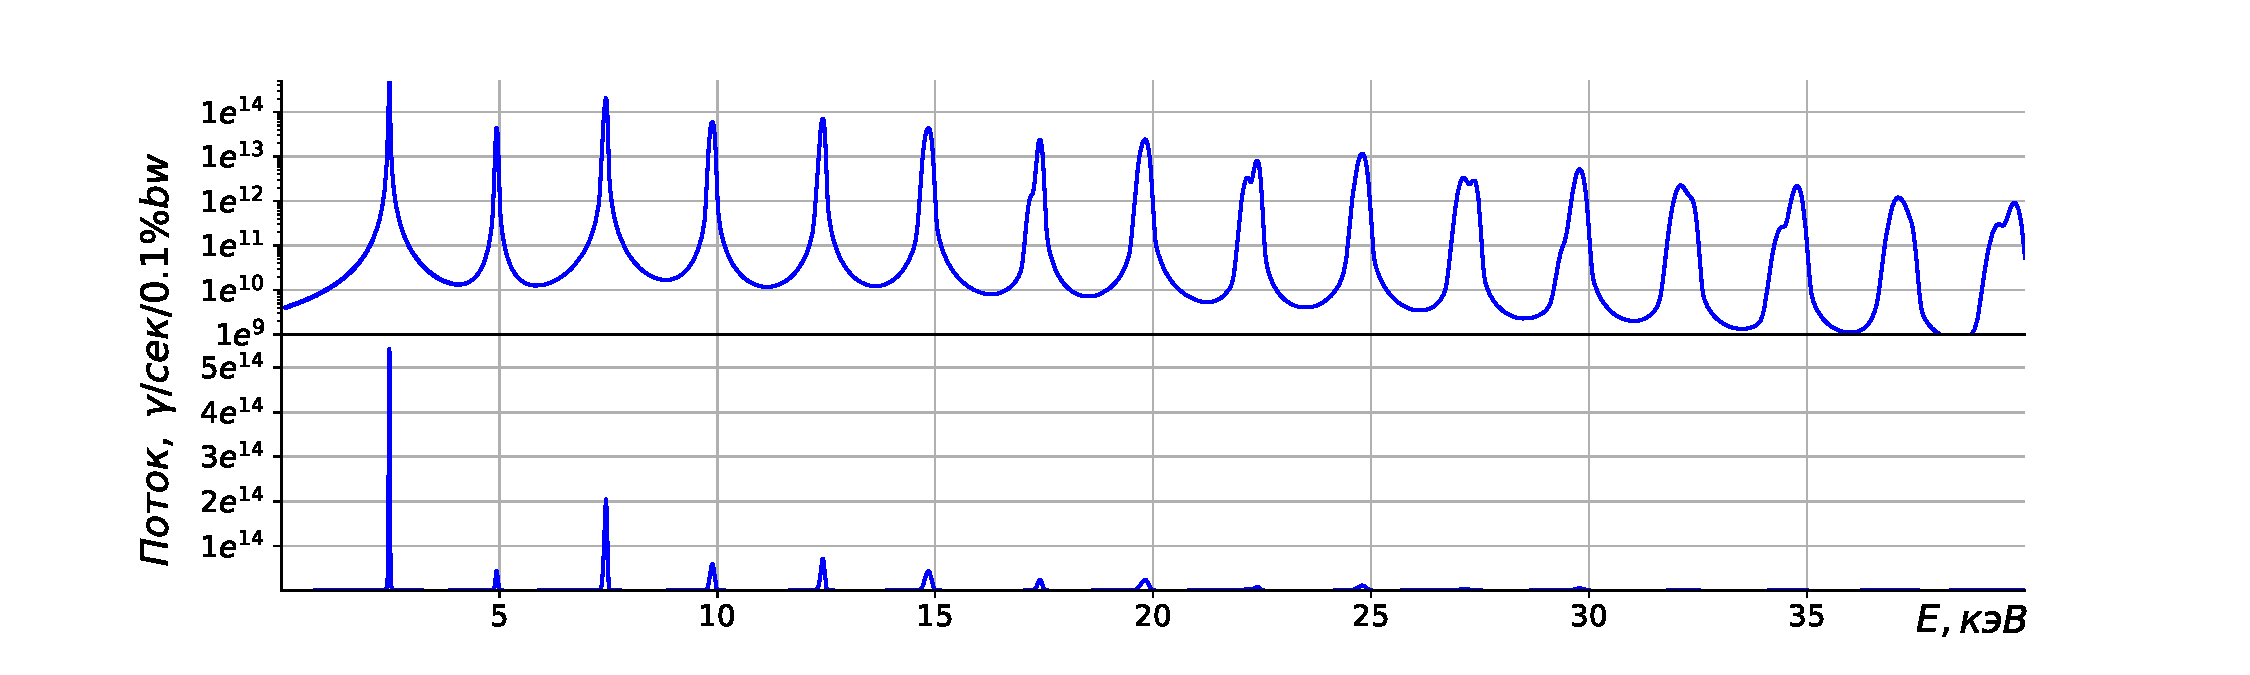
\includegraphics[width=\textwidth]{pic/log_spec_1-2.pdf}
	\caption{Спектр с ондулятора с $K = 1,54$ через апертуру $0,4 \; \textup{мм}$ в логарифмическом масштабе (сверху) и в линейном (снизу) посчитанный в SPECTRA с учётом конечности эмиттанса и энергетического разброса}
	\label{fig:log_spec_1-2}
\end{figure}

\subsection{Оптика станции 1-2}
Оптическая схема станции, в смысле алгоритма расчётов, аналогична станции 1-1, с одним лишь отличием в том, что используется другой тип ондулятора и более низкие рабочие гармоники. На рис.~\ref{fig:OptScheme_1-2} приведена схема станции, совпадающая по структуре со той же схемой для 1-1. 
\begin{figure}[h!]
	\centering  
	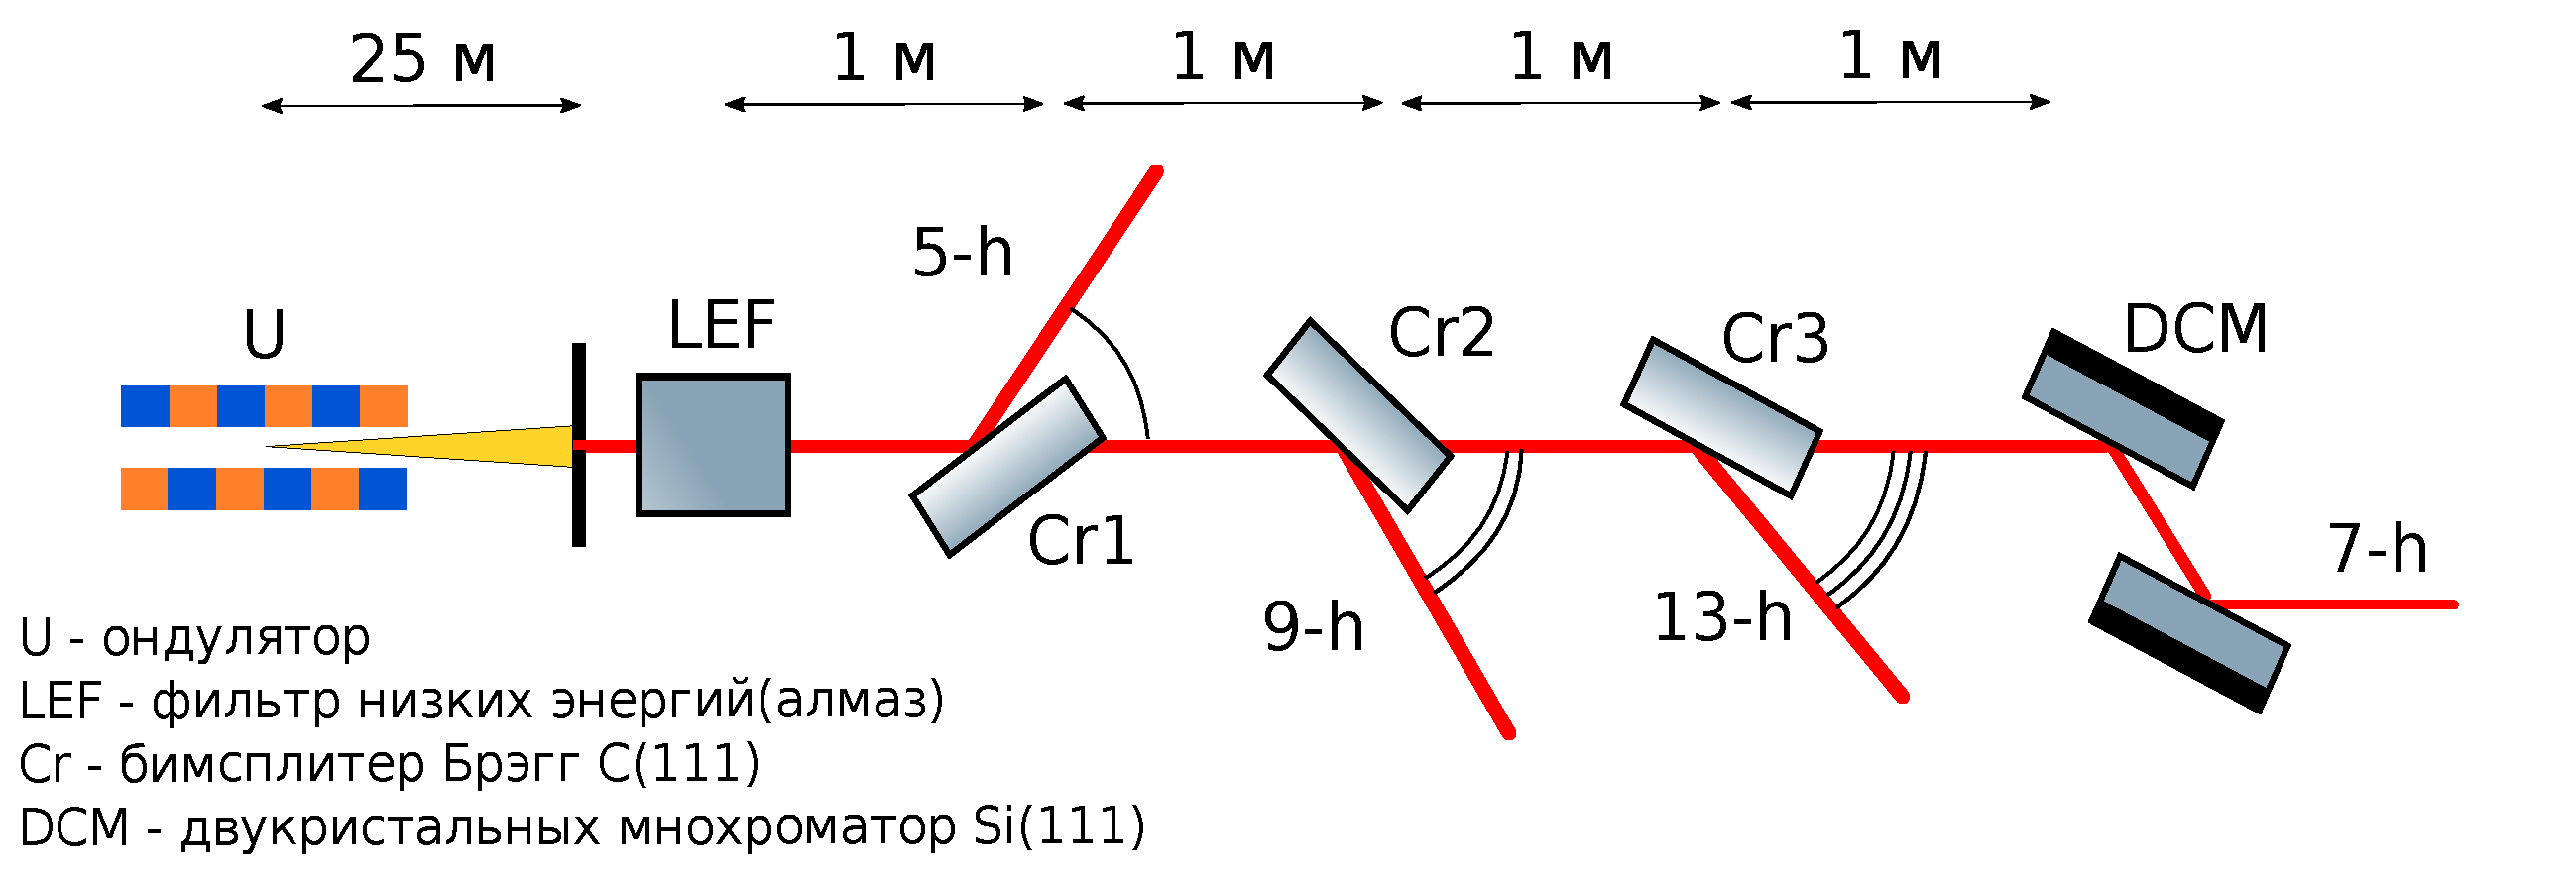
\includegraphics[width=\textwidth]{pic/OptScheme_1-2.pdf}
	\caption{Оптическая схема станции 1-2}
	\label{fig:OptScheme_1-2}  
\end{figure}
На рис.~\ref{fig:full_spec_1-2} приведены удельные тепловые нагрузки на элементы станции. 
%Такое же как и для 1-1 сравнение результатов расчёта полной падающей удельной мощности на первый оптический элемент можно найти на рис.~\ref{fig:power_dens_1-2} в приложении к работе.
\begin{figure}[h!]
	\centering
	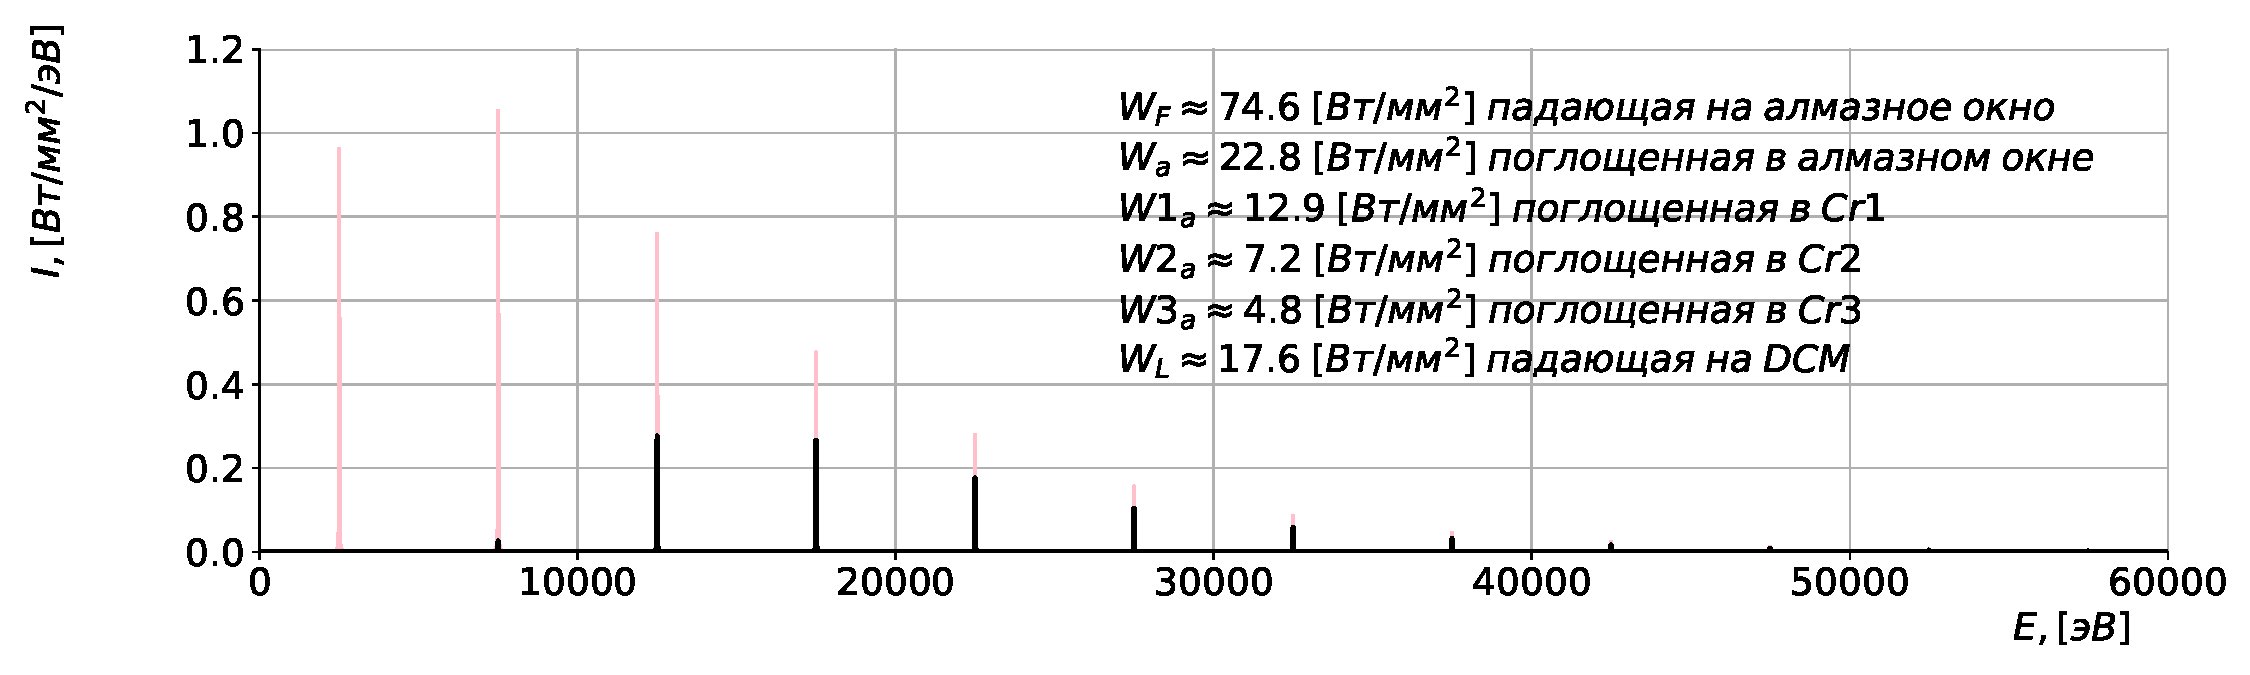
\includegraphics[width=\textwidth]{pic/full_spec_1-2.pdf}
	\caption{Спектр электронного пучка с нулевым эмиттансом падающий на алмазное окно --- розовый цвет, тот же излучение падающее на двукристалльный монохроматор --- чёрный цвет}
	\label{fig:full_spec_1-2}   
\end{figure}

Итого, результаты расчётов: 
\DTLloaddb
[
noheader,
keys={},
headers={
	\shortstack{$n_{harm}$},
	\shortstack{$\sigma_x, [mm]$},
	\shortstack{$\sigma_y, [mm]$},
	\shortstack{$\sigma_x, [\mu rad]$},
	\shortstack{$\sigma_y, [\mu rad]$}}
]
{RMS_before1-2}{tabl_1-2/RMS_before1-2.csv}
\begin{table}[h!]
	\caption{Сечение пучка на входе в первую апертуру (25 м)}
	\sisetup{
		parse-numbers   = false,
		table-number-alignment = right,
		table-figures-integer = 4,
		table-figures-decimal = 4,
		input-decimal-markers = .
	}
	\renewcommand*\dtlrealalign{S}
	\centering
	\DTLdisplaydb{RMS_before1-2}
	\label{table:size_obeam}
\end{table}

\DTLloaddb
[
noheader,
keys={},
headers={
	\shortstack{$n_{harm}$},
	\shortstack{$\theta_{cr}, grad$},
	\shortstack{$d_{eff}, \mu m$},
	\shortstack{$S_{proj}, mm$}}
]
{Cr_angles1-2}{tabl_1-2/Cr_angles1-2.csv}
\begin{table}[h!]
	\caption{Номер гармоники, ориентация кристалла, эффективная толщина алмазного монохроматора, проекция пучка(горизонтальная) }
	\sisetup{
		parse-numbers   = false,
		table-number-alignment = right,
		table-figures-integer = 4,
		table-figures-decimal = 4,
		input-decimal-markers = .
	}
	\renewcommand*\dtlrealalign{S}
	\centering
	\DTLdisplaydb{Cr_angles1-2}
	\label{table:stable}
\end{table}

\DTLloaddb
[
noheader,
keys={},
headers={
	\shortstack{$n_{harm}$},
	\shortstack{$\sigma_x, [mm]$},
	\shortstack{$\sigma_y, [mm]$},
	\shortstack{$\sigma_x, [\mu rad]$},
	\shortstack{$\sigma_y, [\mu rad]$}}
]
{RMS_after1-2}{tabl_1-2/RMS_after1-2.csv}
\begin{table}[h!]
	\caption{Сечение пучка после монохроматоров}
	\sisetup{
		parse-numbers   = false,
		table-number-alignment = right,
		table-figures-integer = 4,
		table-figures-decimal = 4,
		input-decimal-markers = .
	}
	\renewcommand*\dtlrealalign{S}
	\centering
	\DTLdisplaydb{RMS_after1-2}
	\label{table:size_obeam_after}
\end{table}

\DTLloaddb
[
noheader,
keys={},
headers={
	\shortstack{$n_{harm}$},
	\shortstack{$E, eV$},
	\shortstack{$\lambda, [nm]$},
	\shortstack{$ph/s$},
	\shortstack{$ph/s/0.1\%$},
	\shortstack{$\Delta E / E$}}
]
{ph_beam_par_after_cr1-2}{tabl_1-2/ph_beam_par_after_cr1-2.csv}
\begin{table}[h!]
	\caption{Потоки фотонов после соответствующих монохроматоров}
	\sisetup{
		parse-numbers   = false,
		table-number-alignment = right,
		table-figures-integer = 4,
		table-figures-decimal = 4,
		input-decimal-markers = .
	}
	\renewcommand*\dtlrealalign{S}
	\centering
	\DTLdisplaydb{ph_beam_par_after_cr1-2}
\end{table}

\newpage
\section{Станция 1-4 --- <<XAFS-спектроскопия и магнитный дихроизм>>}
\subsection{Вставное устройство}
На вставное устройство станции 1-4 накладываются довольно жёсткие условия, так как на этой станции планируется реализовать две техники XAFS спектроскопии --- обычный EXAS и quick-EXAS. Последняя техника требует довольно широкого спектра до $1 - 1.2 \; \textup{кэВ}$, что не может быть реализованно с помощью обычного планарного ондулятора, ширина спектра которого, определяется количеством периодов и равна порядка: $\Delta \omega / \omega = 10^{-2}$. Для уширения спектра ондуляторного излучения используют так называемую технику тэперинга, изменение магнитного поля некоторым способом или длины периодов ондулятора вдоль траектории электронного пучка.

На станции будет использоваться сверхпроводящий ондулятор с возможность производить сканирование по спектру. Магнитное поле может меняться в широких пределах, посредствам подстройки тока в обмотках сверхпроводящего устройства. Параметры такого ондулятор см. в таблице~\ref{table:und1-4}. 
\begin{table}[h!]
	\caption{Параметры ондулятора для станции 1-4}
	\centering
	\begin{tabular}{c|c|c|c}
		\hline\hline
		\rule{0pt}{3ex}$\mathnormal{B(K), [T]}$   & $\mathnormal{L, [m]}$ & $\mathnormal{d, [mm]}$ &  Рабочие Гармоники       \\ \hline
		\rule{0pt}{3ex}$0.65 - 1.37(1.1 - 2.3)$   & $2.3$                 & $18$        		   & $3 - 13$\\
		\hline\hline
	\end{tabular}
	\label{table:und1-4}
\end{table}
Помимо этого, на  ондулятор накладывается условие того, что рабочие гармоники должны перекрываться, чтобы предоставить пользователям вести непрерывное сканирование по энергии в диапазоне от $4 \; \textup{кэВ}$ до $40 \; \textup{кэВ}$. На рис.~\ref{fig:F_A} представлен спектр с указанными выше $K$ ондулятора, показано эффективное перекрытие рабочих гармоник с большим запасом.
\begin{figure}[h!]
	\begin{minipage}{0.99\textwidth}
		\centering  
		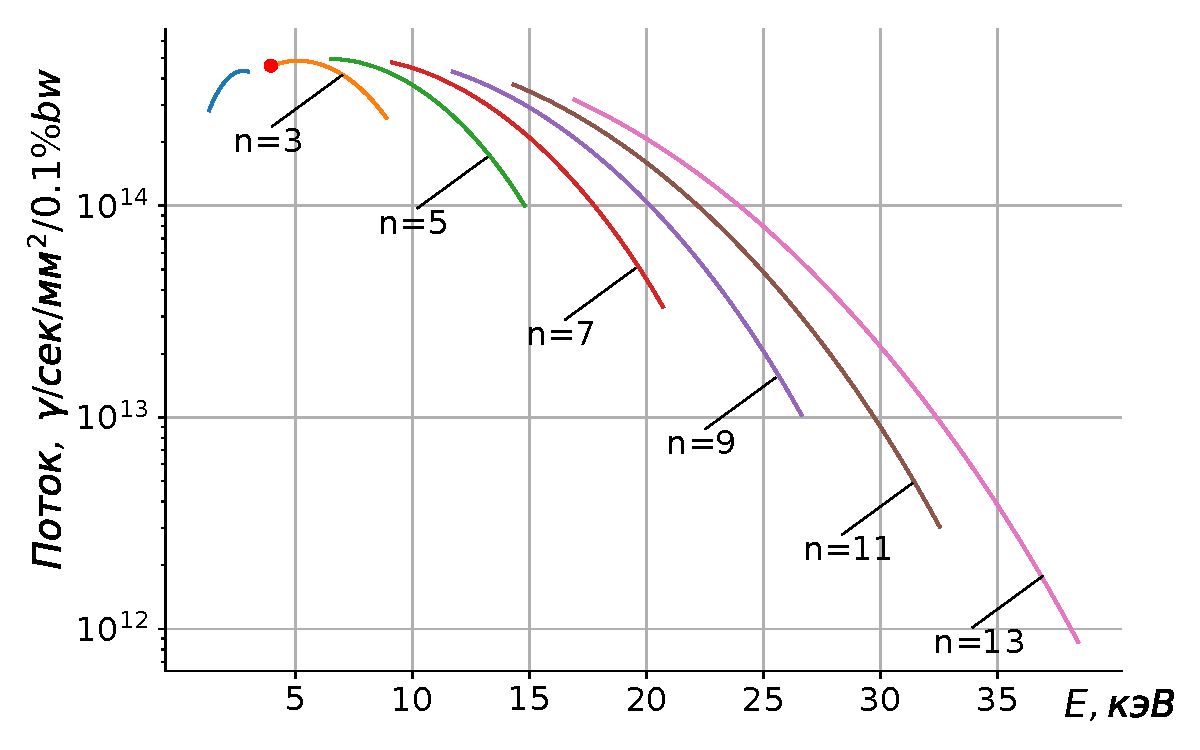
\includegraphics[width=\textwidth]{pic/F_A.pdf}
		\caption{Спектр ондулятора для 1-4 с параметром $K$, меняющемся в диапазоне от $1,1 - 2,3$}
		\label{fig:F_A}  
	\end{minipage}\hfill

	\begin{minipage}{0.99\textwidth}
		\centering
		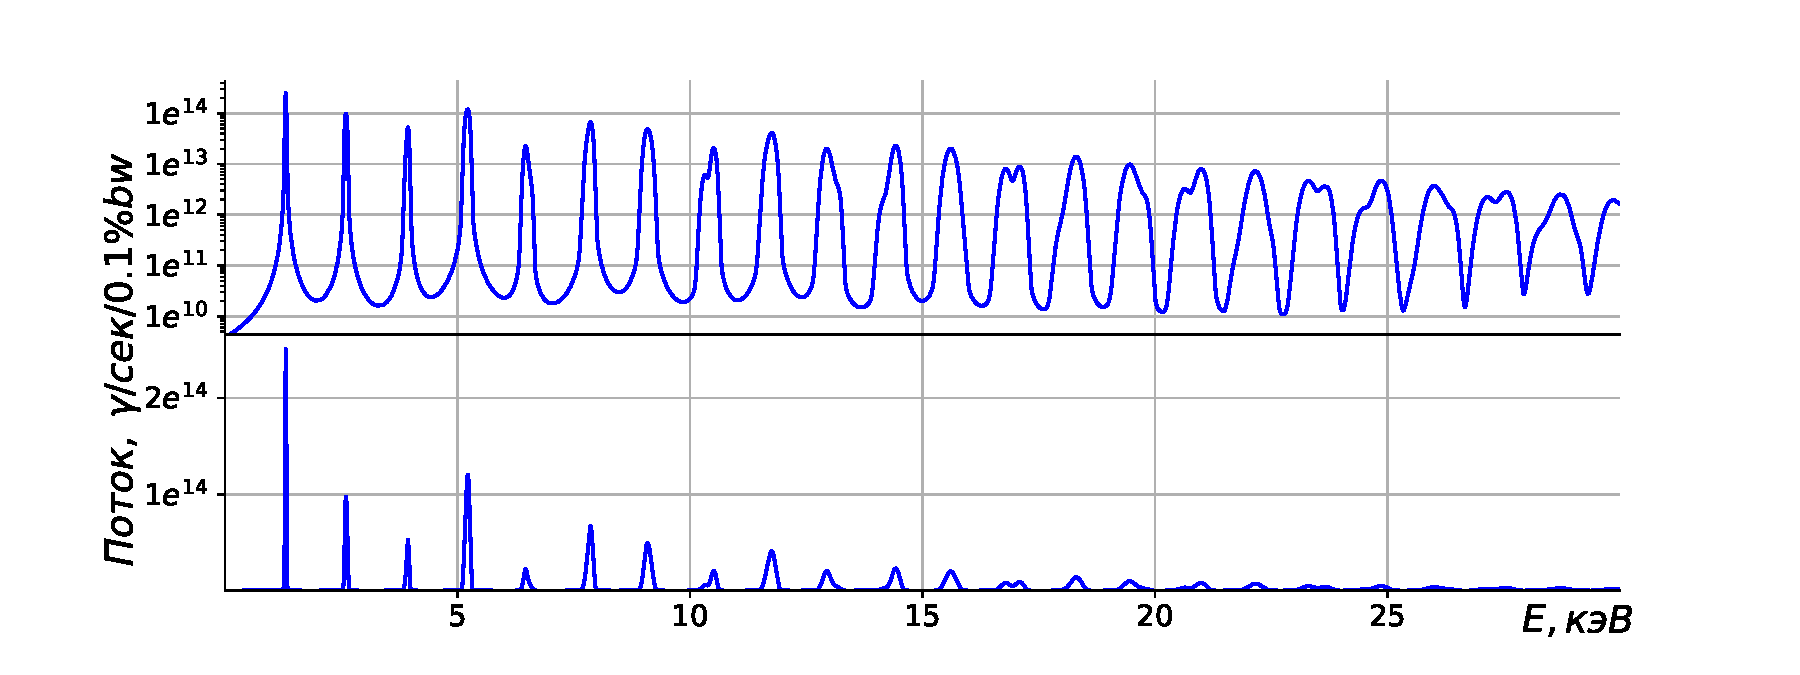
\includegraphics[width=\textwidth]{pic/log_spec_1-4.pdf}
		\caption{Спектр с ондулятора с $K = 2,23$ через апертуру $1 \; \textup{мм}$ в логарифмическом масштабе (сверху) и в линейном (снизу) посчитанный в SPECTRA с учётом конечности эмиттанса и энергетического разброса}
		\label{fig:section_und_SRW}
	\end{minipage}    
\end{figure}


\subsection{Излучение клинообразного ондулятора}
В этой секции мы рассмотрим излучение планарного ондулятора специальной конструкции, который может доставить широкий спектр. Идея состоит в том, что разбить ондулятор на несколько секций с различным магнитным полем в каждой из них, см. рис.~\ref{fig:section_und_sheme}.
\begin{figure}[h]
	\centering  
	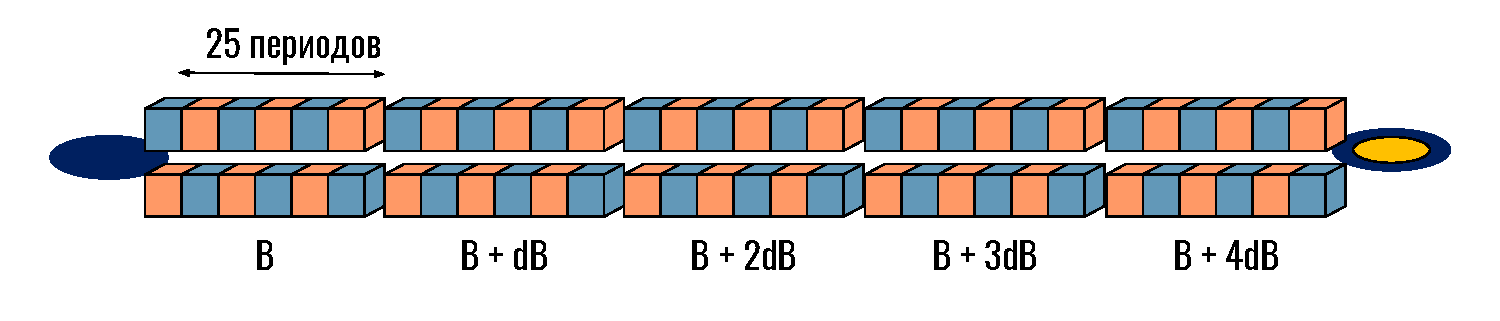
\includegraphics[width=\textwidth]{pic/und.pdf}
	\caption{Ондулятор состоящий из малых ондуляторных секций.}
	\label{fig:section_und_sheme}  
\end{figure}
Такая расстановка, в первом приближении, предполагалось, должна дать набор резонансов, которые сольются в один сплошной спектр. Однако, более детальное рассмотрение показало, что в зависимости от фазы электрона между сегментами, могут проявляться интерференционные эффекты, которые в значительной степени будут изменять форму спектра. 

Выкладки можно начать с модифицированного интеграла~\ref{eq:field_dist_in_integral}, 
\begin{equation}
\begin{array}{lcl}
\vec{\widetilde{E}}_{\bot}(z_0,  \vec{r}_{\bot 0}, \omega) =
\cfrac{\omega eA_{JJ}}{2c^2z_0}\cfrac{K}{\gamma}
\displaystyle\int\limits_{-\lambda_w N/2}^{\lambda_w N/2} dz'
\exp[iCz'] 	\vec{e}_x,
\end{array}	
\end{equation} 
Здесь, для простоты изложения, излучение рассматривается на оси, т.е. $\theta = 0$ от уединённого электрона. В случае секционного ондулятора коэффициент ондуляторности меняется вдоль ондулятора, поэтому $K = K_0 + n\Delta K$, а также $C = C_0 + n\Delta C$, где $n$ --- это номер секции. Где $\Delta {C}$ введено следующим образом, помня $\omega_r = 2c\widetilde{\gamma}^2k_w$:
\begin{equation}
C =k_w\cfrac{\Delta \omega}{\omega_r} = \cfrac{\Delta \omega_r}{2c\gamma}\bigg(1 + \cfrac{(K_0 + n\Delta K)^2}{2}\bigg) \approx \cfrac{\Delta \omega_r}{2c\gamma}\bigg(1 + \cfrac{K^2_0}{2}(1 + \cfrac{n\Delta K}{K_0})\bigg) = C_0 + \Delta C
\end{equation} 
Секций, для определённости, мы возьмём пять, и для удобства нумерацию будем вести $-2, -1, ... , 2$. Поэтому интеграл можно переписать в виде:
\begin{equation}
\begin{array}{lcl}
\vec{\widetilde{E}}_{\bot}(z_0,  \vec{r}_{\bot 0}, \omega) =
\cfrac{\omega eA_{JJ}}{2c^2 \gamma z_0}
\displaystyle\sum\limits_{n =-2}^{2}(K_0 + n\Delta K)
\displaystyle\int\limits_{(2n + 1)L_s/2}^{(2n - 1)L_s/2} dz'
\exp[i(C_0 + n\Delta C)z']	\vec{e}_x,
\end{array}	
\end{equation} 
Взяв интеграл, получим:
\begin{equation}
\begin{array}{lcl}
\vec{\widetilde{E}}_{\bot}(z_0,  \vec{r}_{\bot 0}, \omega) =
\cfrac{\omega eA_{JJ} L_u}{2c^2 \gamma z_0}
\displaystyle\sum\limits_{n =-2}^{2}(K_0 + n\Delta K)
\sinc(\hat{C}/2)e^{in({C}_0 + n\Delta {C})L}	\vec{e}_x,
\end{array}	
\end{equation} 
Возведя в квадрат, получим интенсивность:
\begin{equation}
\begin{array}{lcl}
{\widetilde{I}} =
\bigg(\cfrac{\omega eA_{JJ} L}{2c^2 \gamma z_0}\bigg)^2\bigg[
\displaystyle\sum\limits_{n =-2}^{2}(K_0 + n\Delta K)^2\sinc^2(\hat{C_0} + n\Delta \hat{C}/2) \; + \\

\displaystyle\mathop{\sum\limits_{n, m =-2}^{2}}_{n \neq m}K^2_0\bigg(1 + n\cfrac{\Delta K}{K_0} + m\cfrac{\Delta K}{K_0}\bigg)
\sinc^2(\hat{C}/2)e^{i(n-m)\hat{C}_0 + (n^2 - m^2)\Delta \hat{C}}\bigg],
\end{array}	
\end{equation} 
Полученное выражение можно проинтерпретировать следующим образом: первая сумма есть сумма сдвинутых по соответствующим резонансам $\sinc^2$ функций, вторая сумма отображает интерференцию между различными секциями ондулятора. Данная комбинация приводит к колебаниями в спектре, как показано на рис.~\ref{fig:section_und_analitics} синими пунктирными линиями, чёрной линией отмечена сумма $\sinc^2$ функций без учёта интерференционных слагаемых.
\begin{figure}[h!]
	\centering  
	\begin{minipage}{0.49\textwidth}
		\centering
		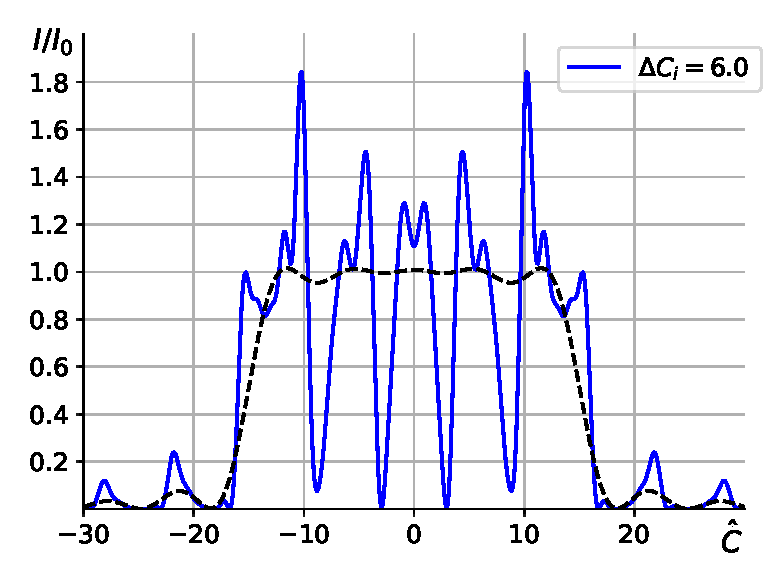
\includegraphics[width=\textwidth]{pic/spec_from_sec_und.pdf}
		\caption{Аналитический результат для электронного пучка с бесконечно малым эмиттансом}
		\label{fig:section_und_analitics}
	\end{minipage}\hfill
	\begin{minipage}{0.49\textwidth}
		\centering
		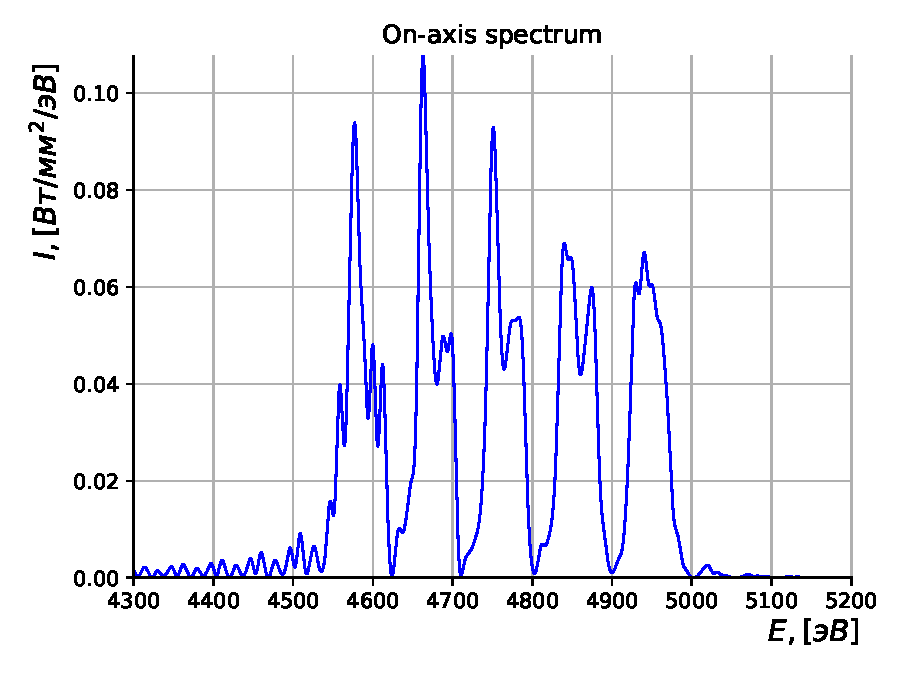
\includegraphics[width=\textwidth]{pic/sim_und_spec.pdf}
		\caption{Симуляция в коде SRW для электронного пучка с бесконечно малым эмиттансом}
		\label{fig:section_und_SRW}
	\end{minipage}    
\end{figure}
На рис.~\ref{fig:section_und_SRW} показан характерный спектр секционного ондулятора посчитанного при помощи симуляционного кода SRW. Далее на рис.~\ref{fig:sim_und_spec_new_mm} представлен спектр с учётом эмиттанса и энергетического разброса в пучке, проинтегрированный по конечной апертуре --- $1 \; \textup{мм}$ на расстоянии $22 \; \textup{м}$.
\begin{figure}[h!]
	\centering  
	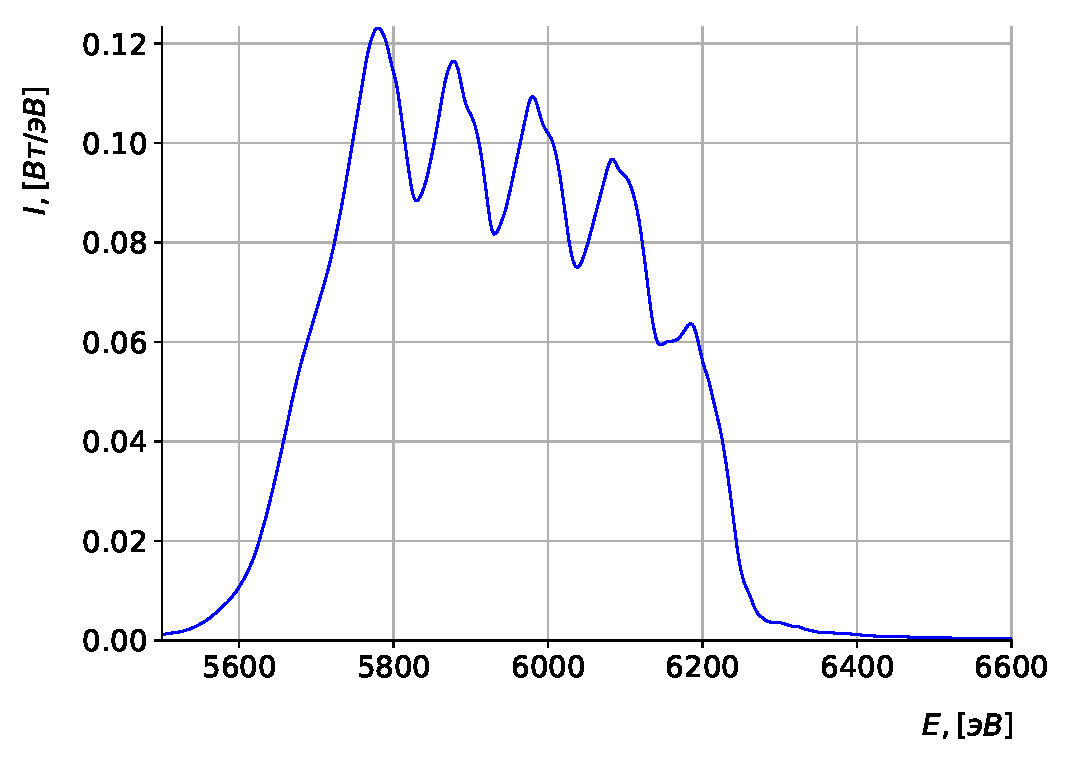
\includegraphics[width=\textwidth]{pic/sim_und_spec_new_mm.pdf}
	\caption{Спектр секционного ондулятора проинтегрированного по конечной апертуре --- $1 \; \textup{мм}$ с учётом конечности эмиттанса и энергетического разброса}
	\label{fig:sim_und_spec_new_mm}  
\end{figure}


\subsection{Оптика станции 1-4}

На рис.~\ref{fig:OptScheme_1-4} представлена оптическая схема станции реализации EXAS спектроскопии, которая состоит из двукристального монохроматора и далее системы зеркал Kirkpatrick-Baez для фокусировки излучения на образец. Для реализации quick-EXAS спектроскопии будет использоваться отдельный монохроматор, но т.к. на данный момент нет консенсуса по концепции ондулятора для этой техники, в данной работе оптическая схема для указанного метода рассматриваться не будет.

\begin{figure}[h]
	\begin{minipage}{0.99\textwidth}
	\centering  
	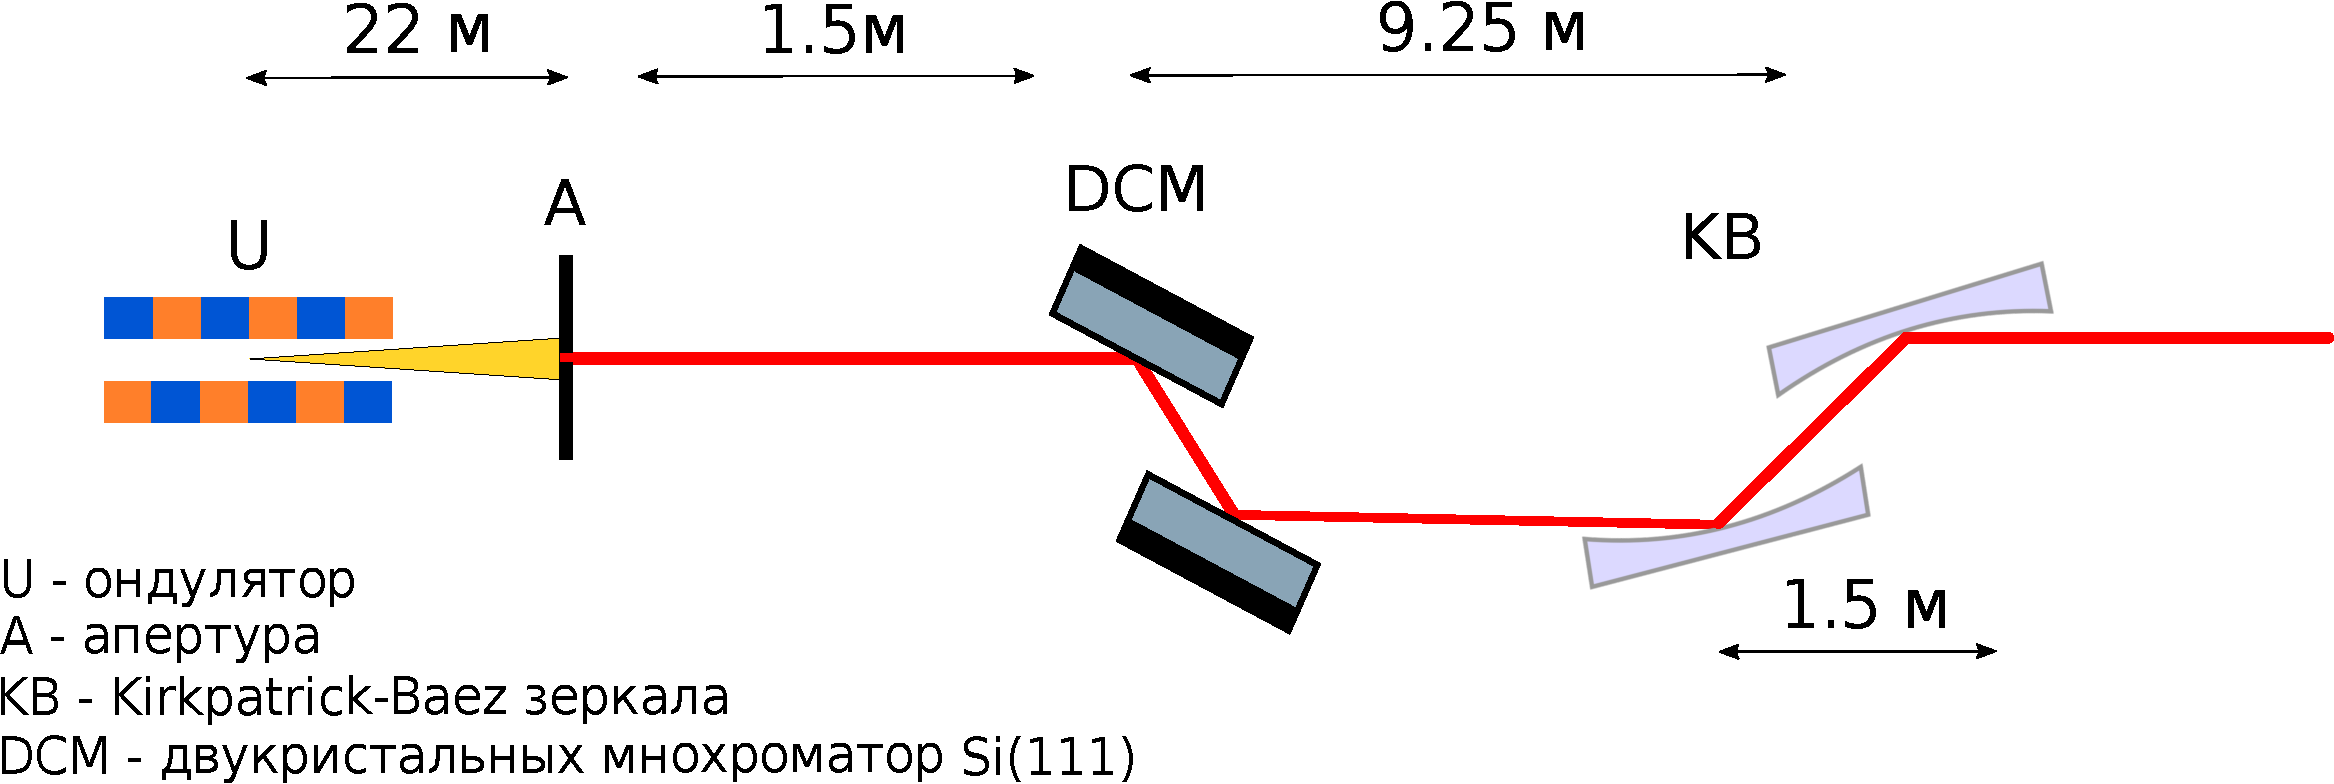
\includegraphics[width=\textwidth]{pic/OptScheme_1-4.pdf}
	\end{minipage}\hfill
	\begin{minipage}{0.3\textwidth}
		\centering
		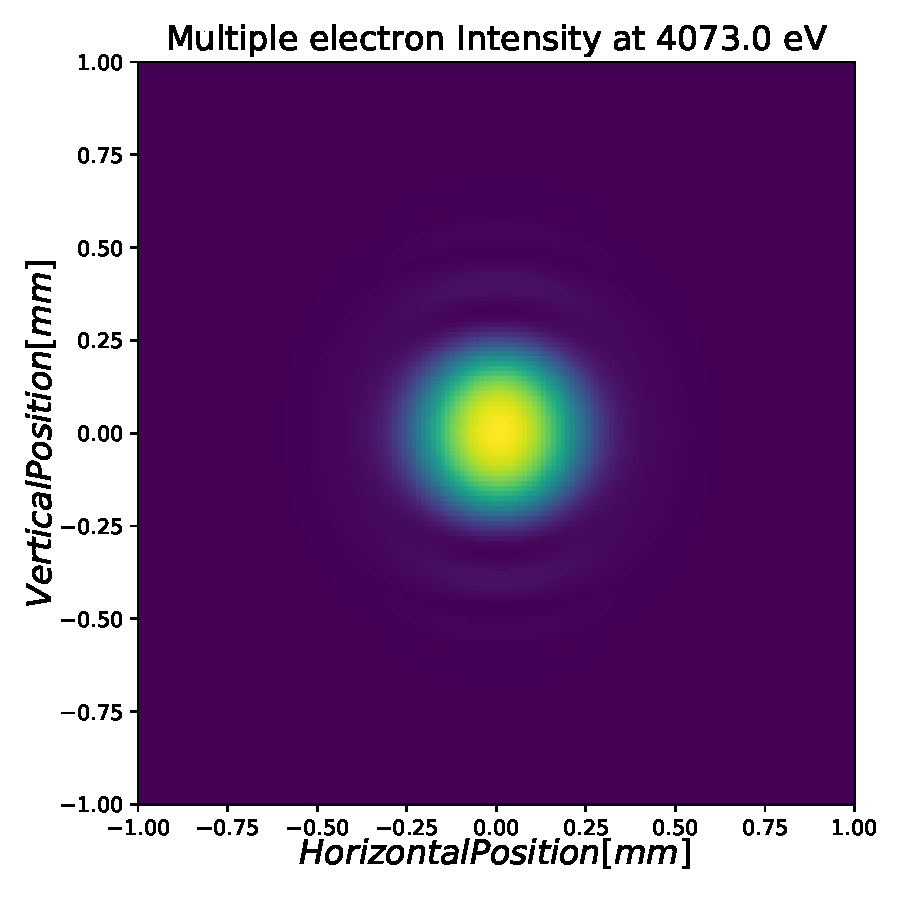
\includegraphics[width=\textwidth]{pic/3_harm_before_optics_2d.pdf}
%		\caption{Сечение пучка до апертуры}
%		\label{fig:3_harm_before_optics_2d}
	\end{minipage}
	\begin{minipage}{0.3\textwidth}
		\centering
		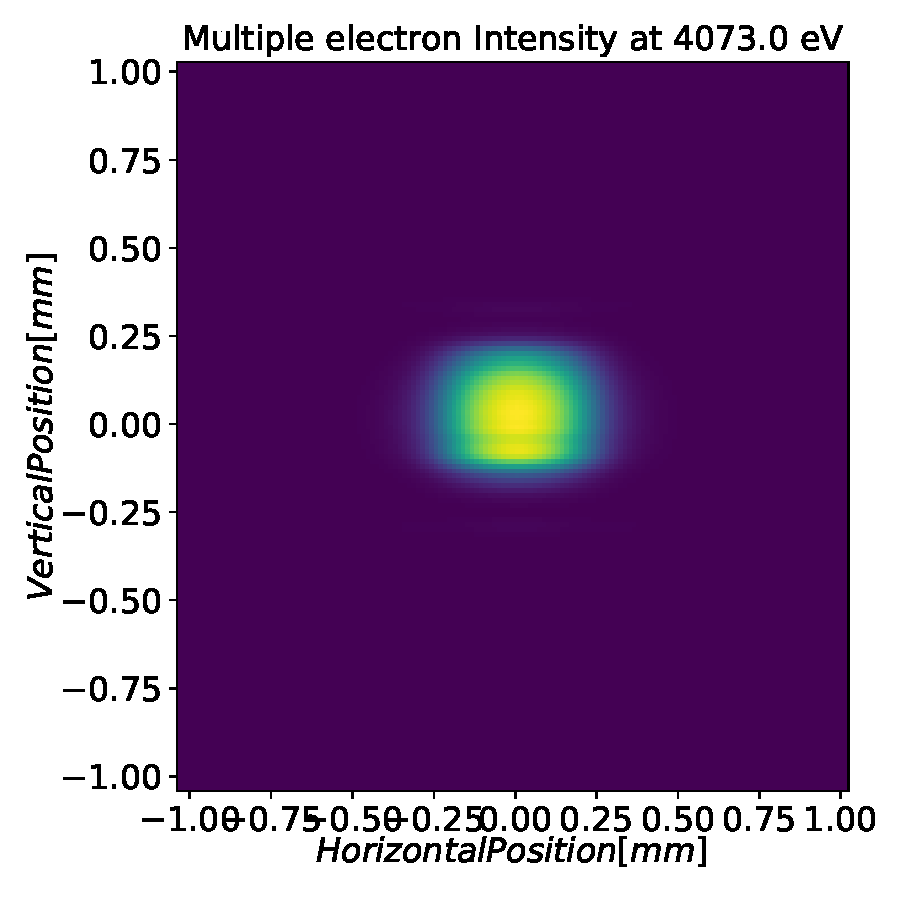
\includegraphics[width=\textwidth]{pic/3_harm_after_DCM_2d.pdf}
%		\caption{Сечение пучка после DCM}
%		\label{fig:3_harm_after_DCM_2d}
	\end{minipage} 
	\begin{minipage}{0.3\textwidth}
		\centering
		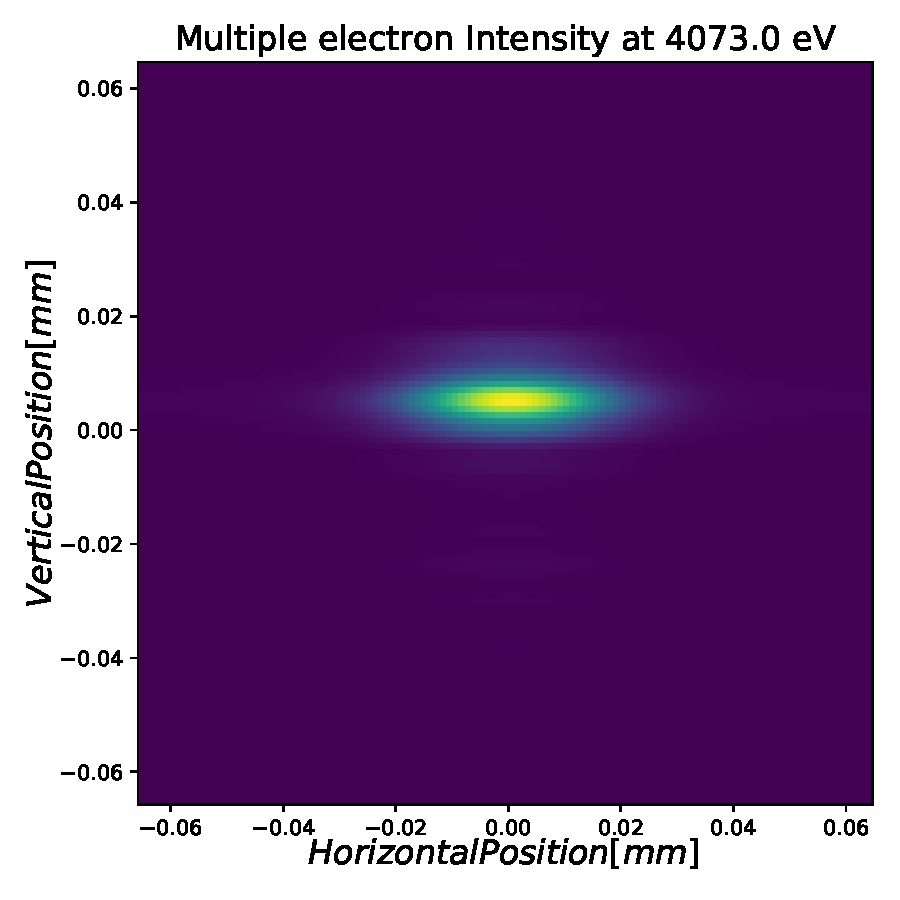
\includegraphics[width=\textwidth]{pic/3_harm_after_Sph_Mir_2d.pdf}
%		\caption{Сечение пучка около фокуса зеркал}
%		\label{fig:3_harm_after_Sph_Mir_2d}
	\end{minipage} 
	\caption{Оптическая схема станции 1-4. Ниже сечения пучка слева на право: на выходе апертуры, на выходе после двукритального монохроматора, на выходе после фокусирующих зеркал}
	\label{fig:OptScheme_1-4}  
\end{figure}


\clearpage                                  % В том числе гарантирует, что список литературы в оглавлении будет с правильным номером страницы
\phantomsection
\addcontentsline{toc}{chapter}{\bibname}	% Добавляем список литературы в оглавление
\hypersetup{ urlcolor=black }               % Ссылки делаем чёрными
%\providecommand*{\BibDash}{}                % В стилях ugost2008 отключаем использование тире как разделителя 
\urlstyle{rm}                               % ссылки URL обычным шрифтом
\insertbiblioother                          % Подключаем Bib-базы
\urlstyle{tt}                               % возвращаем установки шрифта ссылок URL
%\hypersetup{ urlcolor={urlcolor} }          % Восстанавливаем цвет ссылок      % Список литературы
\clearpage
\phantomsection
\addcontentsline{toc}{chapter}{\listfigurename}
\listoffigures									% Список изображений


%%% Список таблиц %%%
% (ГОСТ Р 7.0.11-2011, 5.3.10)
\clearpage
\phantomsection
\addcontentsline{toc}{chapter}{\listtablename}
\listoftables									% Список таблиц
\newpage           % Списки таблиц и изображений (иллюстративный материал)
%\appendix
%% Правка оформления ссылок на приложения:
%http://tex.stackexchange.com/questions/56839/chaptername-is-used-even-for-appendix-chapters-in-toc
%http://tex.stackexchange.com/questions/59349/table-of-contents-with-chapter-and-appendix
%% требует двойной компиляции
\addtocontents{toc}{\def\protect\cftchappresnum{\appendixname{} }%
\setlength{\cftchapnumwidth}{\widthof{\cftchapfont\appendixname~Ш\cftchapaftersnum}}%
}
%% Оформление заголовков приложений ближе к ГОСТ:
\sectionformat{\chapter}[display]{% Параметры заголовков разделов в тексте
    label=\chaptertitlename\ \thechapter,% (ГОСТ Р 2.105, 4.3.6)
    labelsep=20pt,
}
\renewcommand\thechapter{\Asbuk{chapter}} % Чтобы приложения русскими буквами нумеровались
\chapter{Единицы измерения потока фотонов}
В области синхротронного излучения приняты специфические единицы измерения потока фотонов:
\begin{equation}
	\Phi = \cfrac{\gamma}{\textup{сек} \cdot 0.1\%\textup{bw} \cdot \textup{мм}^2}
\end{equation}
Для удобства пользователей этого излучения, была введено необычное единица $0.1\%\textup{bw}$, что можно интерпретировать следующим образом, --- это количество фотонов попавшее в полосу пропускания шириной $0.1\%$ на некоторой фиксированной энергии гамма-квантов, т.е., например, для энергии $1000 \textup{eV}$ ширина полосы будет в диапазоне $999,5 - 1000,5 \textup{eV}$. Данная единица была введена, для удобства оценок потоков, после прохождения излучения через кристаллические монохроматоры и решёточные монохроматоры, полосы пропускания которых как раз составляют порядка $10^{-3} - 10^{-4}$. 

Иногда возникает потребность, для удобства, перевести эти единицы, например, к следующему виду:
\begin{equation}
\Phi = \cfrac{\gamma}{\textup{сек} \cdot \textup{eV} \cdot \textup{мм}^2}
\end{equation} 
Сделать это можно следующим образом, необходимо поточено умножить спектральное распределение на множитель $\cfrac{0.1 \% \cdot E_{ph}}{1\textup{eV}}$, что даст необходимые единицы измерения. Далее, спектр можно привести к:
\begin{equation}
\Phi = \cfrac{W}{\textup{eV} \cdot \textup{мм}^2},
\end{equation} 
Так спектральное распределение легко интегрировать, чтобы получить, например, полную плотность мощности излучения и делать оценки тепловых нагрузок на оптические элементы.
\chapter{Краткий обзор дифракции на кристаллах}
В этой главе мы кратко дадим основные результаты кинетической и динамической теории дифракции. Основные кристаллы используемы на источниках синхротронного излучения --- это $Si$ (кремний), $C$ (алмаз) и реже $Ge$ (германий). Виду кубической кристаллической решётки эти кристаллы относительно просты при рассмотрение динамики отражение и преломления на кристаллических плоскостях. Для нас важны такие свойства кристаллов, как способность преобразовать относительно широкой спектр ондуляторного излучения в излучение с относительной монохроматичностью до $\Delta E/ E \sim 10^{-4}$. Также мы дадим основную информация по поглощательным способностям кристаллов
\section{Симметричное брэгговское отражение от идеально кристалла}
Длины волн, которые отвечают резонансу при отражении падающего под углом $\theta$ к плоскости кристалла излучения, даётся законом Брэгга:  
%пропорциональный $\gamma / nN$, где $n$ --- номер гармоники излучения, $N$ --- число периодов ондулятора, а $\gamma$ --- гамма фактор релятивистского электрона
\begin{equation}
	m\lambda = 2d\sin\theta,
\end{equation}
где $d$ --- расстояние между плоскостями от которых происходит отражение, $m$ --- некоторое положительно целое число. Однако динамическая и кинематическая теории дифракции уточнаю данные результат и вносят конечную угловую и/или по энергии ширину, в которую кристалл может принять излучение, а также некоторый сдвиг, относительно предполагаемого брэгговского угла.  Кривая, которая описывает отражательную способность кристалла, называется кривой Дарвина, именно она определяет угловой и/или энергетический акцептанс излучения. На рис.~\ref{fig:bragg_R} показаны характерные кривые отражение для алмаза и кремния. 
\begin{figure}
	\centering  
	\begin{minipage}{0.49\textwidth}
		\centering
		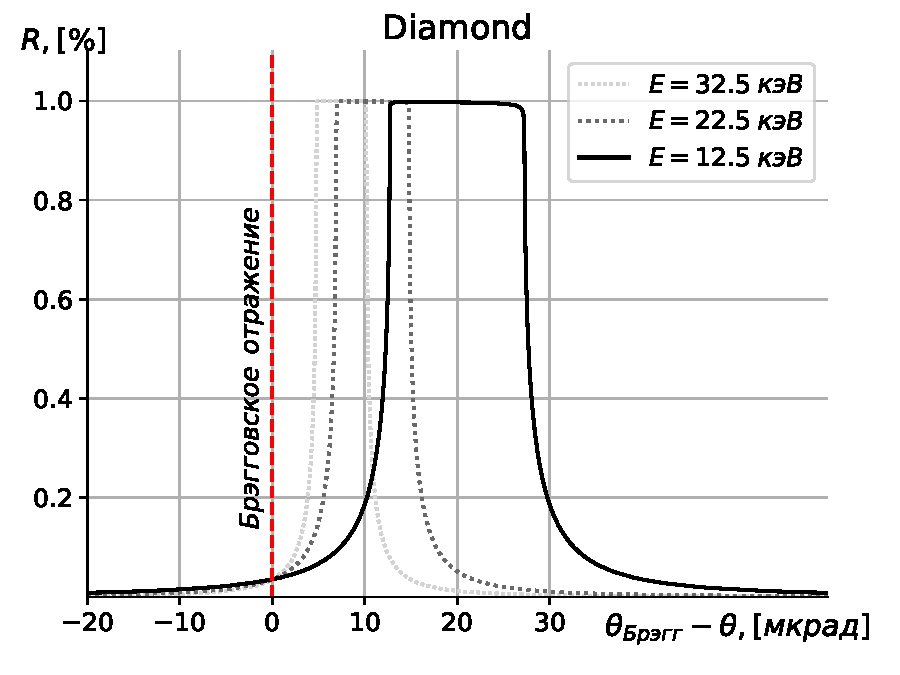
\includegraphics[width=\textwidth]{pic/Diamond_bragg_R.pdf}
		\caption{Кривая брегга для алмаза на разных энергиях}
		\label{fig:bragg_R}
	\end{minipage}\hfill
	\begin{minipage}{0.49\textwidth}
		\centering
		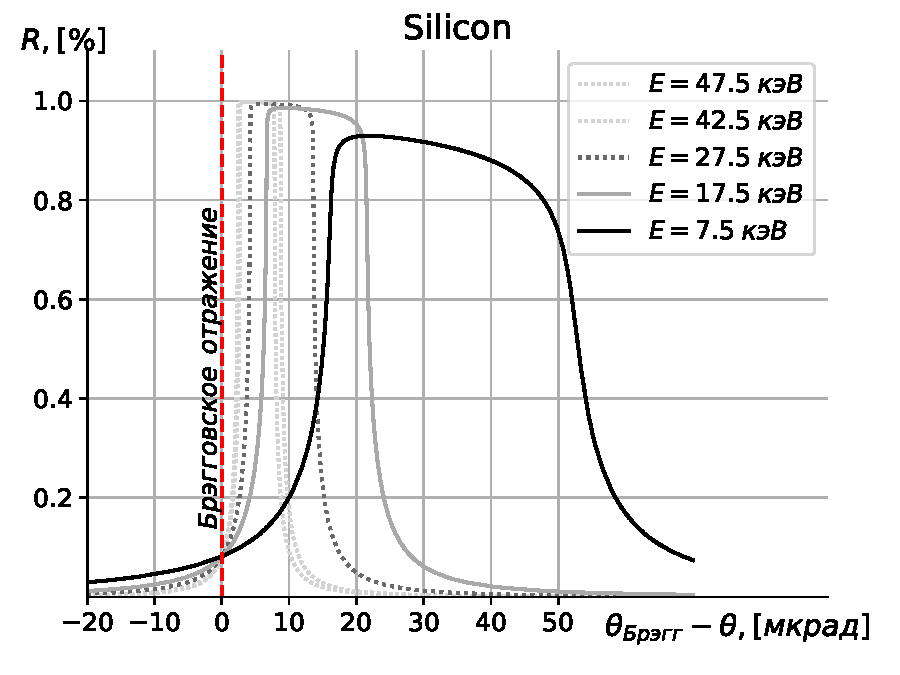
\includegraphics[width=\textwidth]{pic/Silicon_bragg_R.pdf}
		\caption{Кривая брегга для кремния на разных энергиях}
		\label{fig:bragg_T}
	\end{minipage}    
\end{figure}
По ним видно, чем больше энергия подающего пучка излучения, тем  кривая уже и ближе к даваемому законом брэгга углу. При расчёте кристаллов монохроматоров этот факт необходимо учитывать, для эффективной работы кристалла и уменьшения тепловых нагрузок, угловая расходимость кристалла должна входить в акцептанс кристалла, иначе излучение поглотится в кристалле, что крайне нежелательно. Кривые ассиметричны по правому краю, теория дифракции объясняет данный факт большим поглощением на низких энергиях.

В целом, данной информации достаточно, чтобы иметь первое представление о разработке оптических трактов синхротронного излучения. Для дальнейшего чтения и углубления знаний в данном вопросе могут быть полезны следующие книги \cite{als2011elements}, \cite{authier2006dynamical}.

\section{Поглощательные способности кристаллов}
Одним из полезных применений кристаллов в рентгеновском диапазоне есть их фильтрующая способность, отрезать низкие энергии, в особенности для алмазных кристаллов, которые, по мимо всего, имеют хорошую теплопроводность, что способствуют быстрому теплоотводу. На рис.~\ref{fig:bragg_T} представлена кривая поглощения 100 мкм кристалла алмаза. Подобные кристаллы устанавливают перед первыми оптическими элементами, что в значительной степени снижает тепловые нагрузки, подавляя низшие гармоники, в нашем случае ондуляторного излучения. 
\chapter{Дополнительные графики} \label{AppendixA}

\chapter{Примеры программного кода} \label{AppendixB}

\section{Подраздел приложения}\label{AppendixB1}

\normalsize% возвращаем шрифт к нормальному
        % Приложения

\end{document}
